\documentclass[11pt]{book}
\usepackage{fullpage}
\usepackage{palatino}
\usepackage{amsfonts,amsmath,amssymb}

% Packages for displaying code:
\usepackage{listings}
\usepackage{textcomp}
\usepackage{color}

% Color settings used in the code below:
\definecolor{dkgreen}{rgb}{0,0.6,0}
\definecolor{gray}{rgb}{0.5,0.5,0.5}
\definecolor{mauve}{rgb}{0.58,0,0.82}

% Settings for the formatting of the code on display:
\lstset{frame=tb,
  language=R,
  aboveskip=3mm,
  belowskip=3mm,
  showstringspaces=false,
  columns=flexible,
  basicstyle={\small\ttfamily},
  numbers=none,
  numberstyle=\tiny\color{gray},
  keywordstyle=\color{blue},
  commentstyle=\color{dkgreen},
  stringstyle=\color{mauve},
  breaklines=true,
  breakatwhitespace=true,
  tabsize=3
}

% Packages for Figures:
% Without conversion of eps to pdf:
% \usepackage{graphicx}
% With conversion of eps to pdf,
% which depends on platform.
\ifx\pdftexversion\undefined
    \usepackage[dvips]{graphicx}
\else
    \usepackage[pdftex]{graphicx}
    \usepackage{epstopdf}
    \epstopdfsetup{suffix=}
\fi

\usepackage{subfig}

% Package for displaying inline verbatim commands in footnotes.
\usepackage{fancyvrb}

% This allows pdflatex to print the curly quotes in the
% significance codes in the output of the GAM.
\UseRawInputEncoding

%%%%%%%%%%%%%%%%%%%%%%%%%%%%%%%%%%%%%%%%
\begin{document}
%%%%%%%%%%%%%%%%%%%%%%%%%%%%%%%%%%%%%%%%



\pagestyle{empty}
{\noindent\bf Spring 2023 \hfill Brandon~Parmanand}
\vskip 16pt
\centerline{\bf University of Central Florida}
\centerline{\bf College of Business}
\vskip 16pt
\centerline{\bf QMB 6911}
\centerline{\bf Capstone Project in Business Analytics}
\vskip 10pt
\centerline{\bf Solutions:  Problem Set \#11}
\vskip 32pt
\noindent



\pagebreak
\chapter{Introduction}
%\documentclass[11pt]{book}
%\usepackage{palatino}
%\usepackage{amsfonts,amsmath,amssymb}
%
%\begin{document}
%\pagestyle{empty}
%{\noindent\bf Spring 2022 \hfill Firstname M.~Lastname}
%\vskip 16pt
%\centerline{\bf University of Central Florida}
%\centerline{\bf College of Business}
%\vskip 16pt
%\centerline{\bf QMB 6912}
%\centerline{\bf Capstone Project in Business Analytics}
%\vskip 10pt
%\centerline{\bf Solutions:  Problem Sets \#1 \& 2}
%\vskip 32pt
%
%This example has sections for each article in Problem Set \#1.

\section{Introduction}

In this paper I analyze the prices from sales of house. 
My aim is to investigate whether different charactersitics of different homes affect the pricing and whether a home is a rental or owner occuppied affects on pricing.

In the following pages, I will investigate these questions and
ultimately fit a model for the price of houses. 
To understand the dynamics of a sample selection model, 
it is worthwhile to understand the research related to these questions. 



\section{Economic Theory}

\subsection{Market for Lemons}

Akerlof's description of the market for lemons is a long-standing contribution to the understanding of asymmetric information. 


\subsection{Characteristic Theory}

The paper by Lancaster (1966) is a contribution to economic theory in which he makes the case for a sound theory of consumer choice, 
in which the consumer's preferences are defined on the characteristics of different goods, 
rather than the quantities of uniformly-defined goods.


\subsection{Hedonic Pricing Models}

Rosen (1974) builds on the work of Lancaster (1966)
by providing an empirical framework for estimating the value
of products based on their characteristics. 



\section{Empirical Framework}

\subsection{Tobit Models}

Heckman (1979) described sample selection models as a model specification question.

Amemiya (1984) summarized the variaous types of Tobit models
and provides a review of research with applications of these models. 
Lee and Trost (1978) is a well-known application to housing markets, 
which incorporates the fact that the residents make a decision
to either own or rent a home before buying. 


% \end{document}

\pagebreak
\chapter{Data Description}

\section{Data Description}

This analysis follows the scripts in the  \texttt{Code} folder to produce a more accurate model for house prices with the data from \texttt{HomeSales.dat} in the \texttt{Data} folder. 
The dataset includes the following variables.
\begin{table}[h!]
\begin{tabular}{l l l}

$year\_built_i$ & = & the year in which the house was constructed \\
$num\_beds_i$ & = & the number of bedrooms in the hosue \\
$num_baths_i$ & = & the number of bathrooms in the house \\
$floor\_space_i$ & = & the area of floor space in the house, in square feet  \\
$lot_size_i$ & = & the area of lot on which the house was built, in square feet \\
$has\_garage_i$ & = & an indicator for whether the house has a garage\\ %, $0$ otherwise \\
$has\_encl\_patio_i$ & = & an indicator for whether the house has an enclosed patio \\ %, $0$ otherwise \\
$has\_security\_gate_i$ & = & an indicator for whether the house is accessed through a security gate\\ %, $0$ otherwise \\
$has\_pool_i$ & = & an indicator for whether the house has a pool \\ %, $0$ otherwise \\
$transit\_score_i$ & = & an integer to represent the convenience of transportion options \\ %, $0$ otherwise \\
$school\_score_i$ & = & an integer to represent the quality of the schools in the county \\ %, $0$ otherwise \\
$type\_of\_buyer_i$ & = & a categorical variable to indicate the type of buyer which is either owner occupied or rental \\ %, $0$ otherwise \\
$price_i$ & = & the price at which the home was sold \\ %, $0$ otherwise \\

\end{tabular}
\end{table}
%



\pagebreak
\chapter{Analysis of the Dependent Variable}
%\documentclass[11pt]{book}
%\usepackage{palatino}
%\usepackage{amsfonts,amsmath,amssymb}
% \usepackage{graphicx}
%
%
%\ifx\pdftexversion\undefined
%    \usepackage[dvips]{graphicx}
%\else
%    \usepackage[pdftex]{graphicx}
%    \usepackage{epstopdf}
%    \epstopdfsetup{suffix=}
%\fi
%
%\usepackage{color}
%
%\begin{document}
%
%%%%%%%%%%%%%%%%%%%%%%%%%%%%%%%%%%%%%%%%
% Problem Set 3
%%%%%%%%%%%%%%%%%%%%%%%%%%%%%%%%%%%%%%%%
%
%\pagestyle{empty}
%{\noindent\bf Spring 2023 \hfill Brandon~Parmanand}
%\vskip 16pt
%\centerline{\bf University of Central Florida}
%\centerline{\bf College of Business}
%\vskip 16pt
%\centerline{\bf QMB 6911}
%\centerline{\bf Capstone Project in Business Analytics}
%\vskip 10pt
%\centerline{\bf Solutions:  Problem Set \#2}
%\vskip 32pt
%\noindent
%
\section*{Assignment Description}
% 
This assignment focuses on the analysis of the dependent variable, price with regards to whether it is owner occupied or a rental property.

%
\begin{figure}[h!]
  \centering
  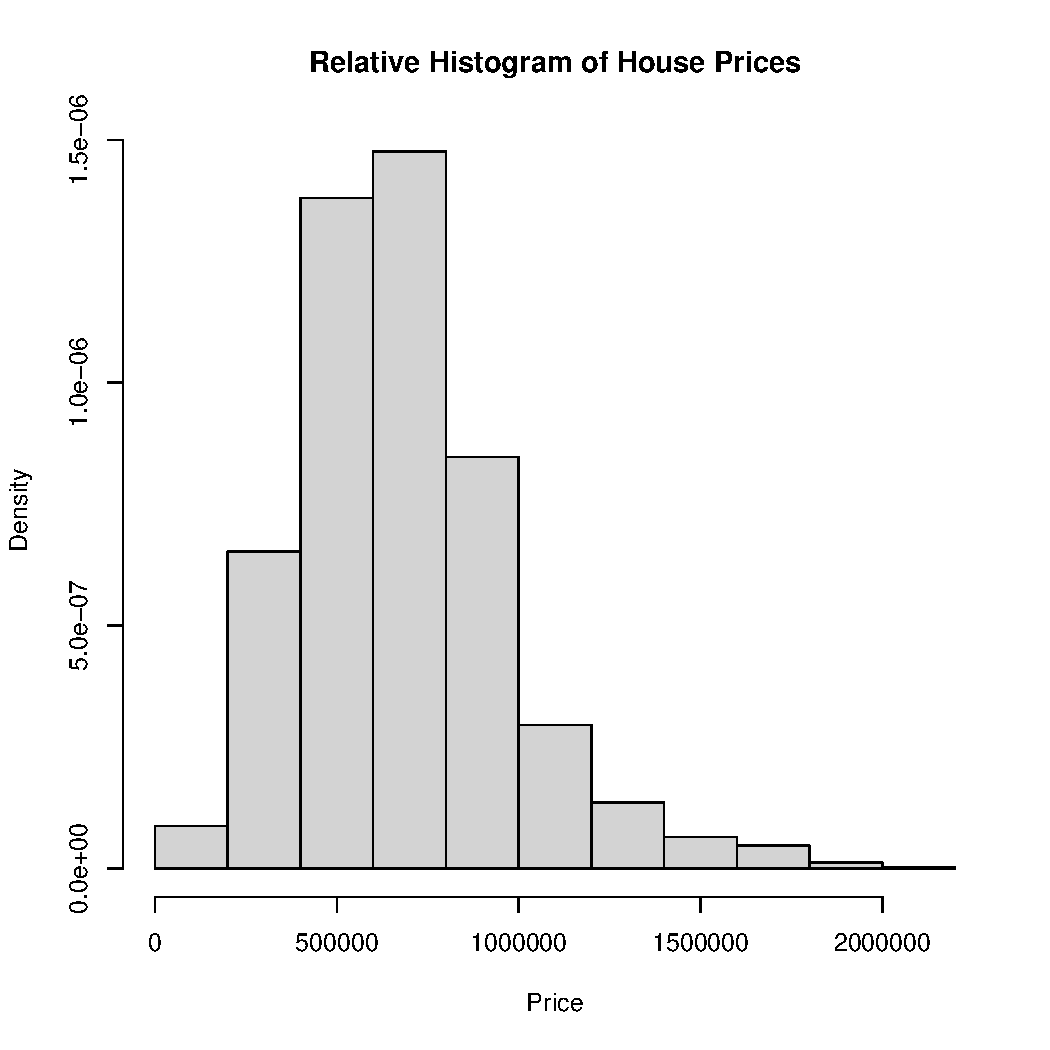
\includegraphics[scale = 0.5, keepaspectratio=true]{../Figures/hist_prices}
  \caption{Relative Histogram of House Prices} \label{fig:hist_prices}
\end{figure}
%
%
\begin{figure}[h!]
  \centering
  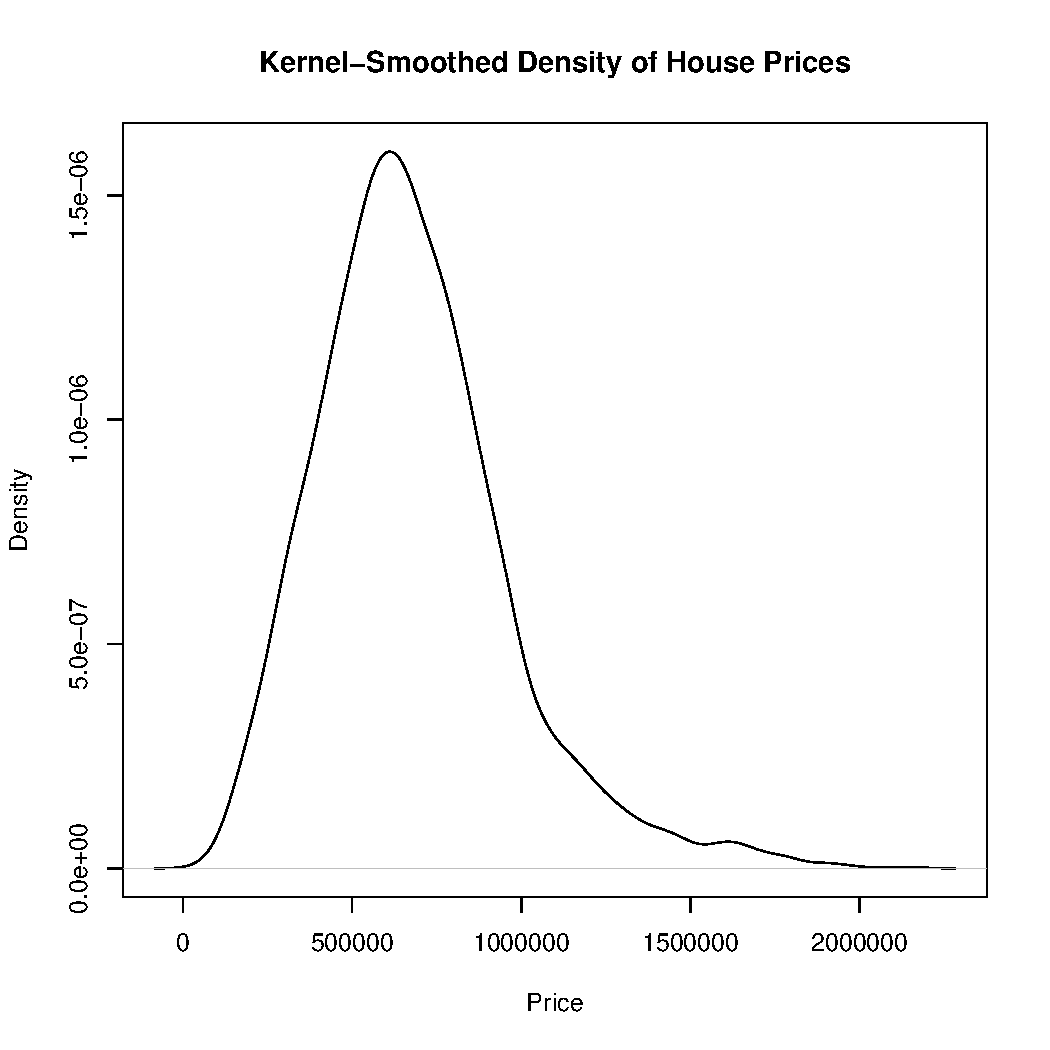
\includegraphics[scale = 0.5, keepaspectratio=true]{../Figures/density_Price}
  \caption{Relative Density of House Prices} \label{fig:density_Price}
\end{figure}
%
%

\begin{figure}[h!]
  \centering
  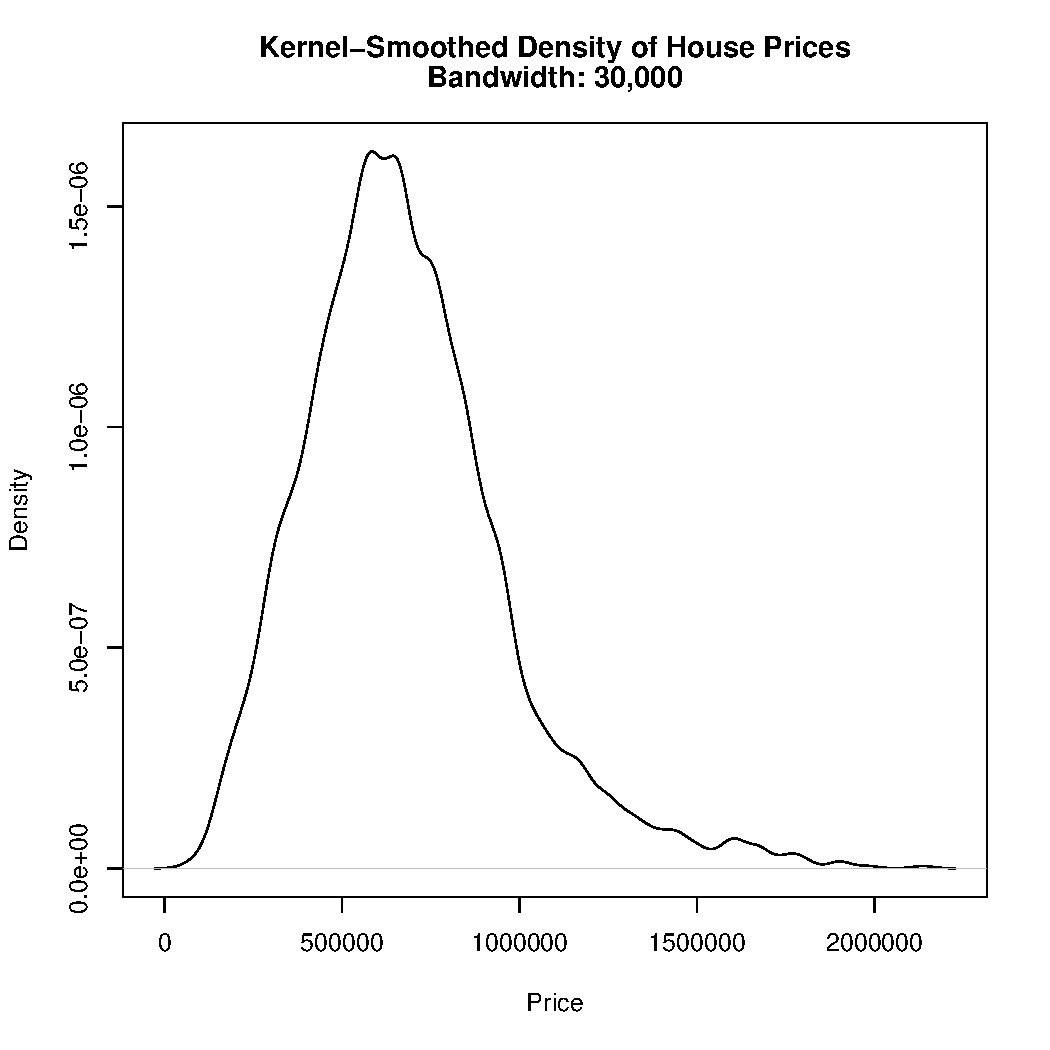
\includegraphics[scale = 0.5, keepaspectratio=true]{../Figures/density_Price_bw30000}
  \caption{Relative Density of House Prices w/ BW = 30,000} \label{fig:density_Price_bw30000}
\end{figure}
%
%
\begin{figure}[h!]
  \centering
  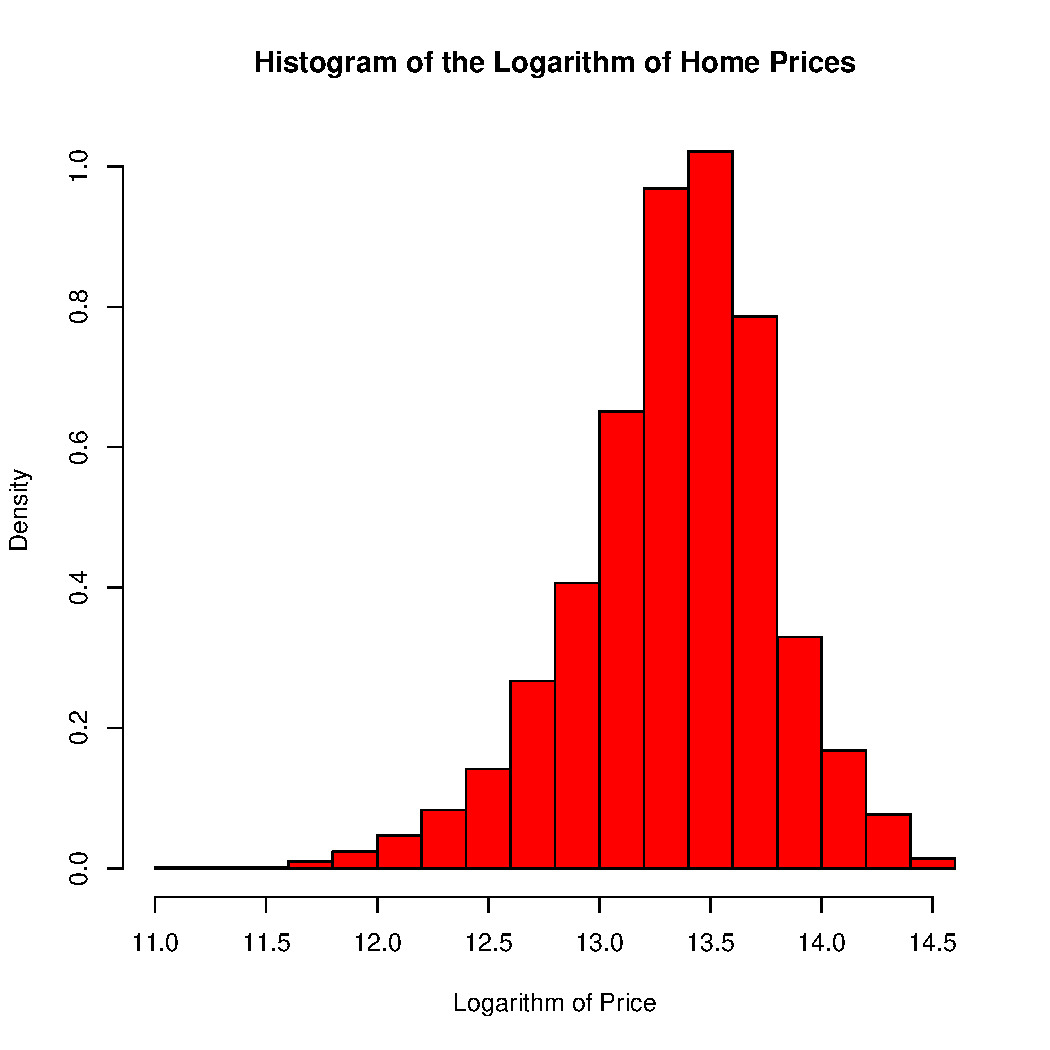
\includegraphics[scale = 0.5, keepaspectratio=true]{../Figures/hist_log_price}
  \caption{Relative Histogram of the House Log Prices} \label{fig:hist_log_price}
\end{figure}
%
%
\begin{figure}[h!]
  \centering
  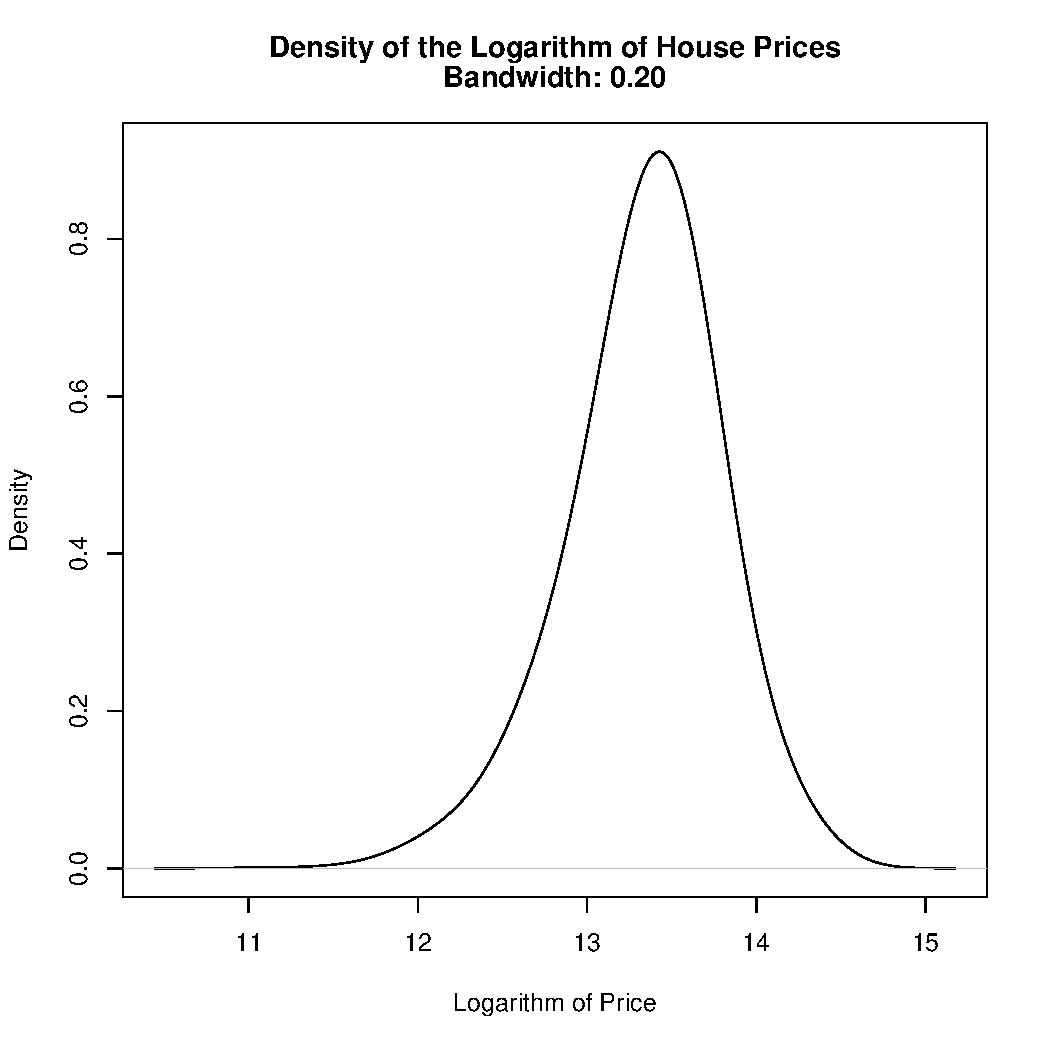
\includegraphics[scale = 0.5, keepaspectratio=true]{../Figures/density_log_saleprice_bw020}
  \caption{Relative Density of House Log Prices w/ BW=0.20} \label{fig:density_log_saleprice_bw020}
\end{figure}
%
%
\begin{figure}[h!]
  \centering
  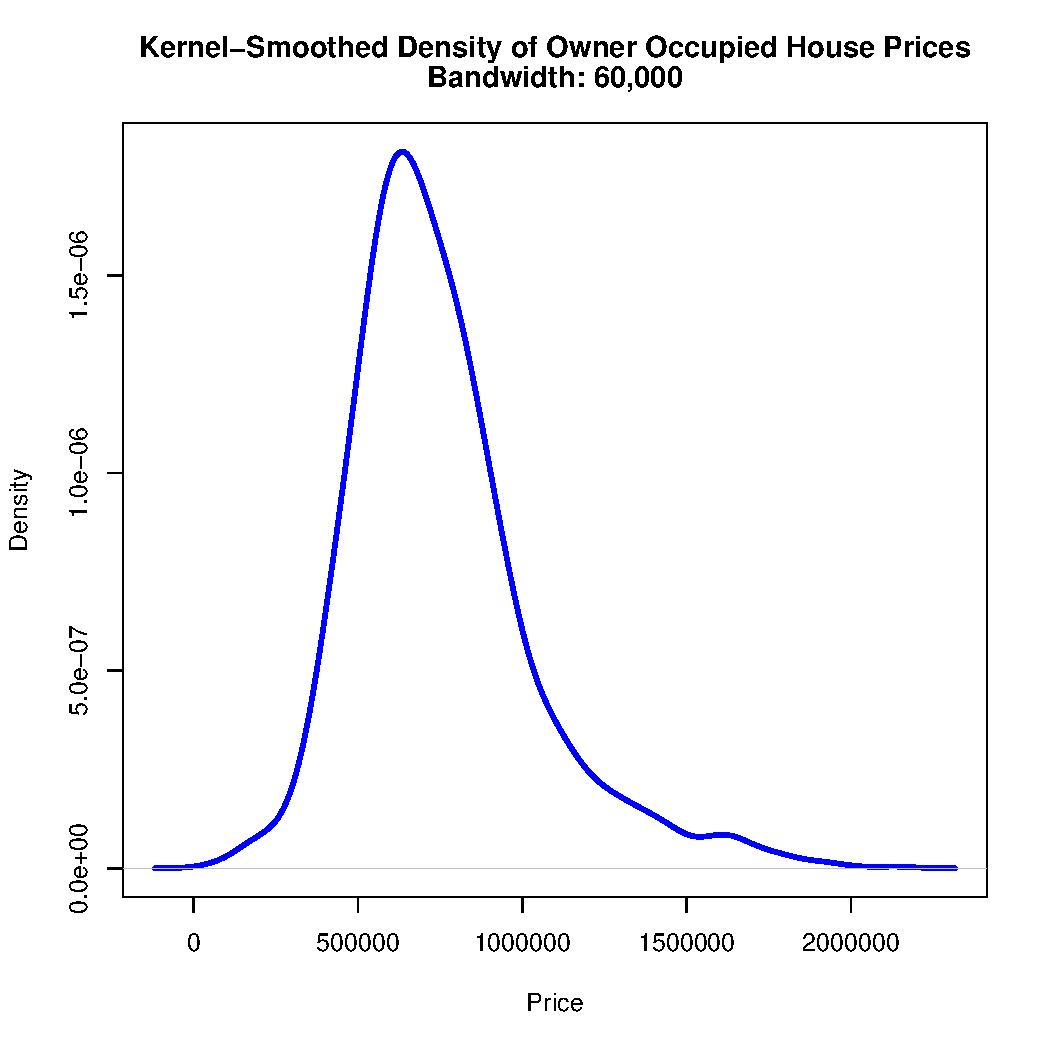
\includegraphics[scale = 0.5, keepaspectratio=true]{../Figures/density_Price_OO}
  \caption{Relative Density of Owner Occupied House Prices w/ BW=60,000} \label{fig:density_Price_OO}
\end{figure}
%
%
\begin{figure}[h!]
  \centering
  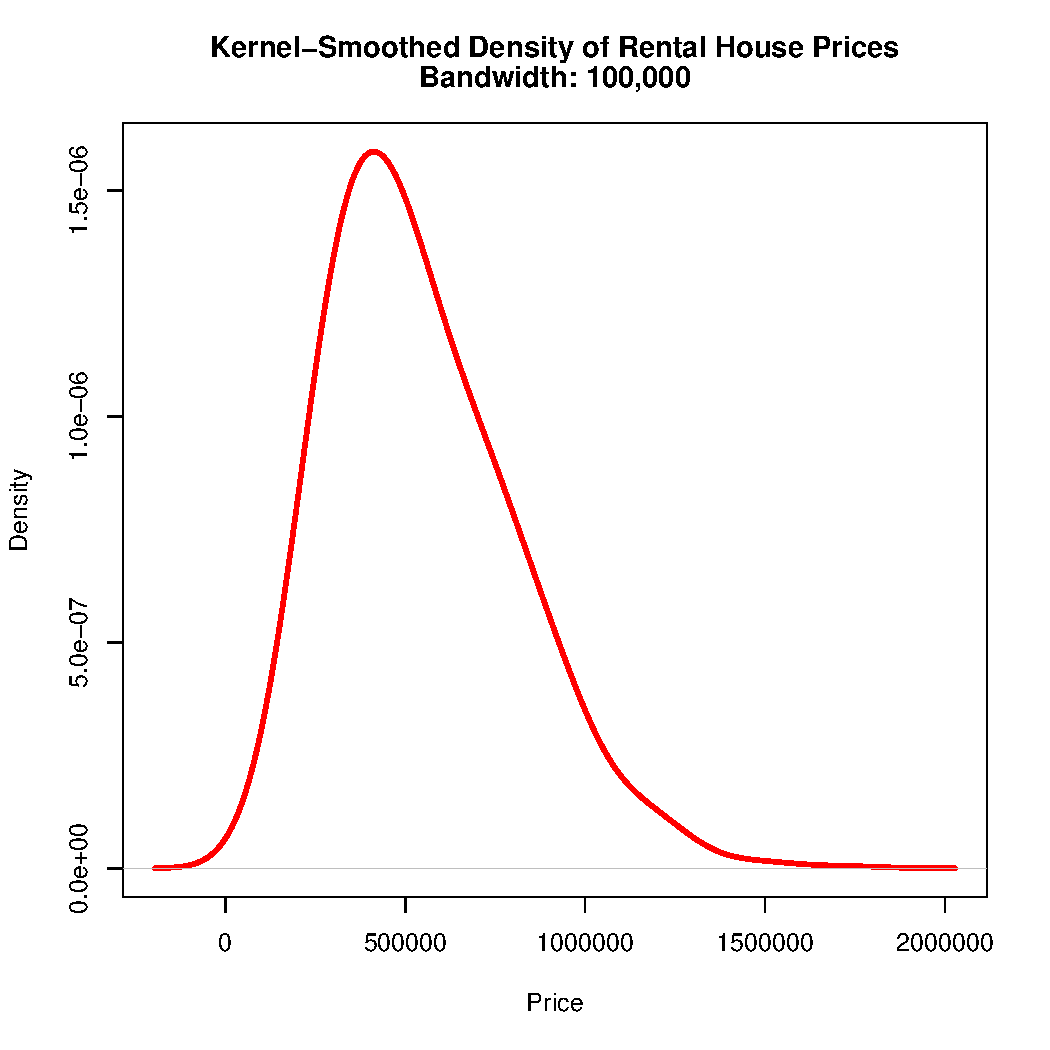
\includegraphics[scale = 0.5, keepaspectratio=true]{../Figures/density_Price_Rental}
  \caption{Relative Density of Rental House Prices w/ BW = 100,000} \label{fig:density_Price_Rental}
\end{figure}
%
%
\begin{figure}[h!]
  \centering
  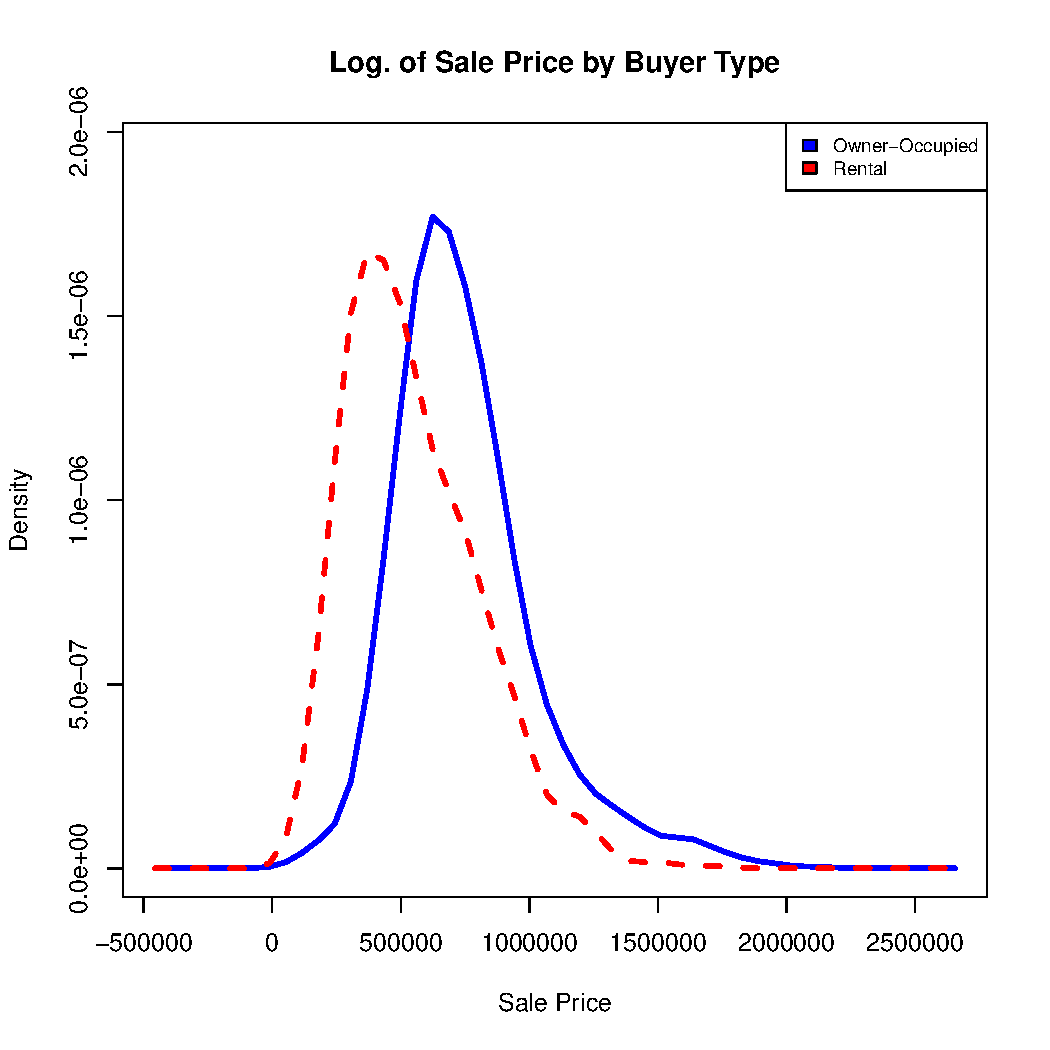
\includegraphics[scale = 0.5, keepaspectratio=true]{../Figures/dens_by_owner}
  \caption{Relative Density of House Prices of Buyer type} \label{fig:dens_by_owner}
\end{figure}
%
%
\begin{figure}[h!]
  \centering
  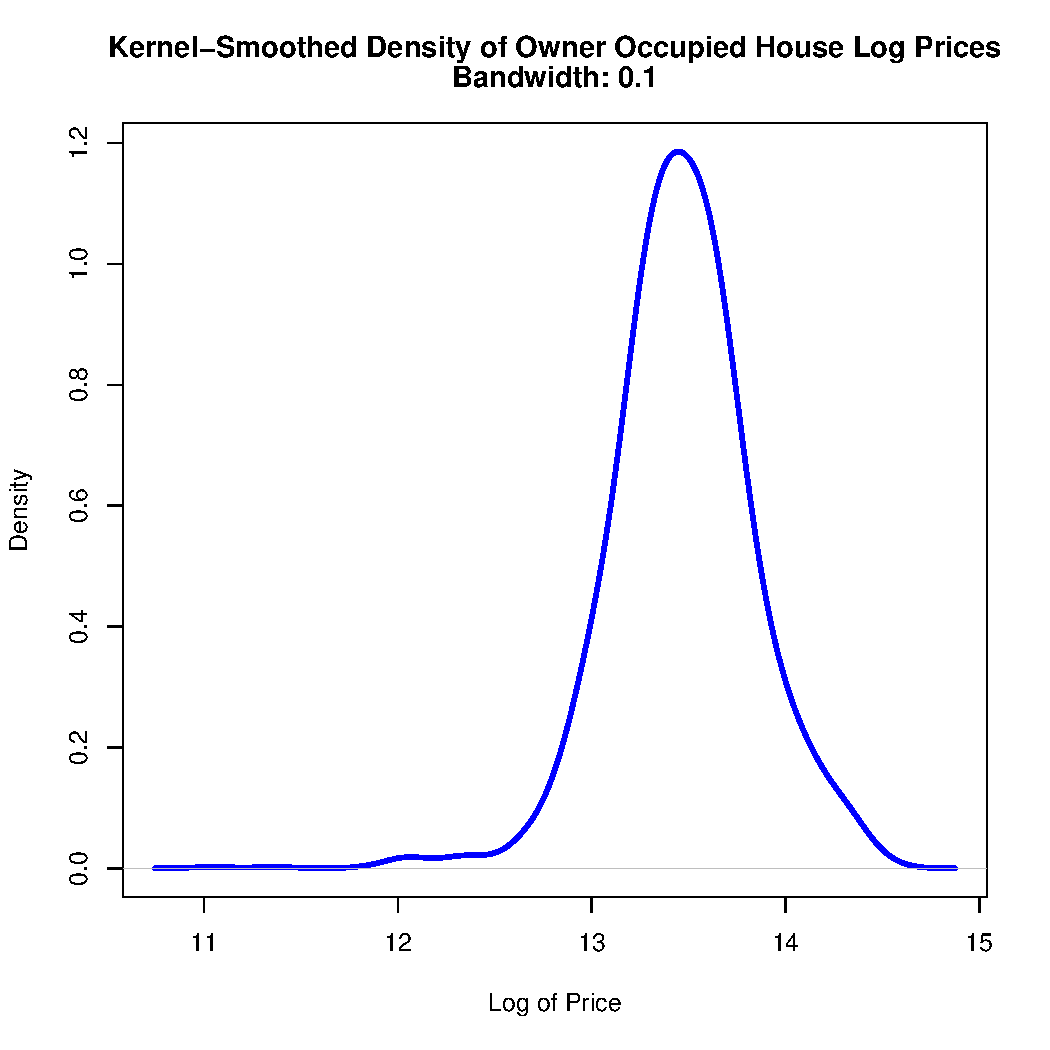
\includegraphics[scale = 0.5, keepaspectratio=true]{../Figures/log_density_Price_OO}
  \caption{Relative Density of Owner Occupied House Log Prices BW=0.1} \label{fig:log_density_Price_OO}
\end{figure}
%
%
\begin{figure}[h!]
  \centering
  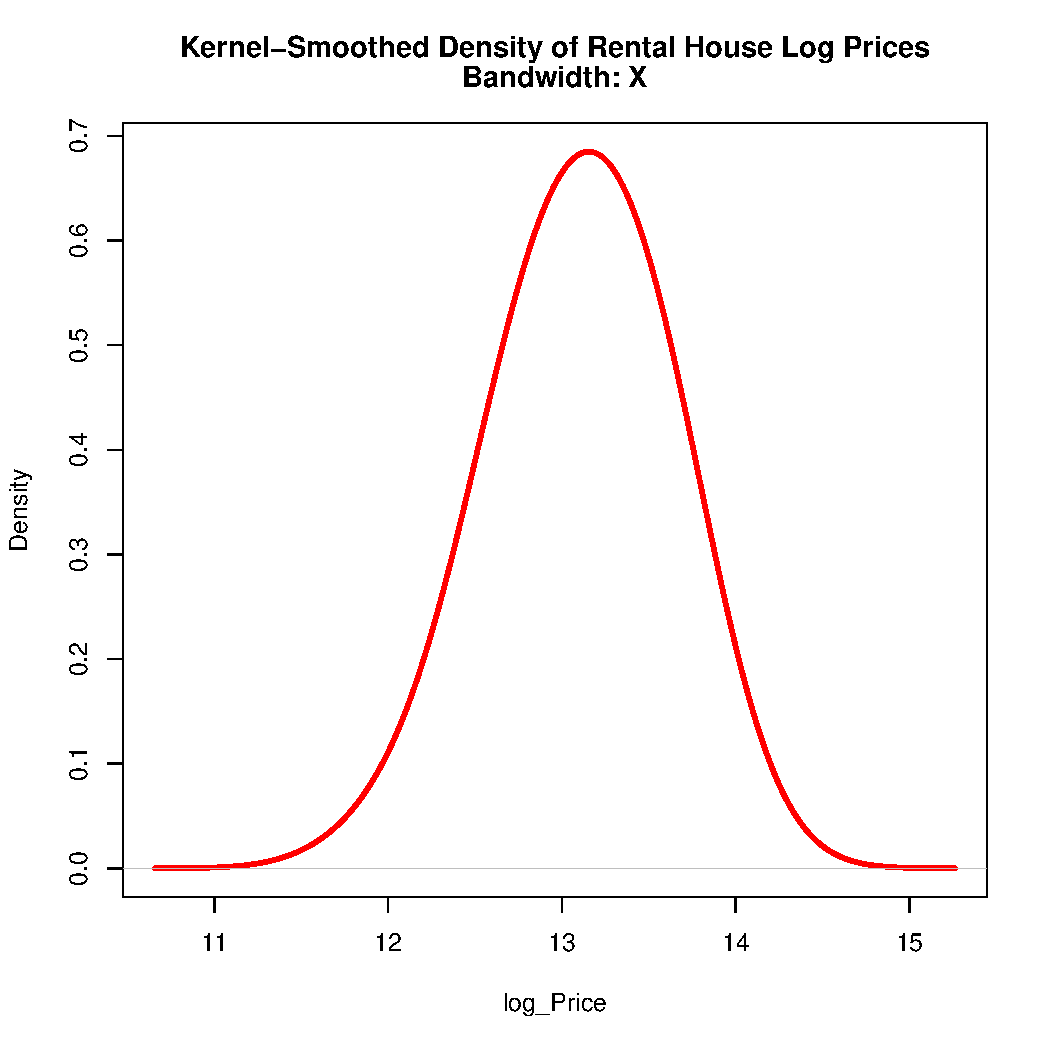
\includegraphics[scale = 0.5, keepaspectratio=true]{../Figures/log_density_Price_Rental}
  \caption{Relative Density of Rental House Log Prices BW=0.3} \label{fig:log_density_Price_Rental}
\end{figure}
%
%
\begin{figure}[h!]
  \centering
  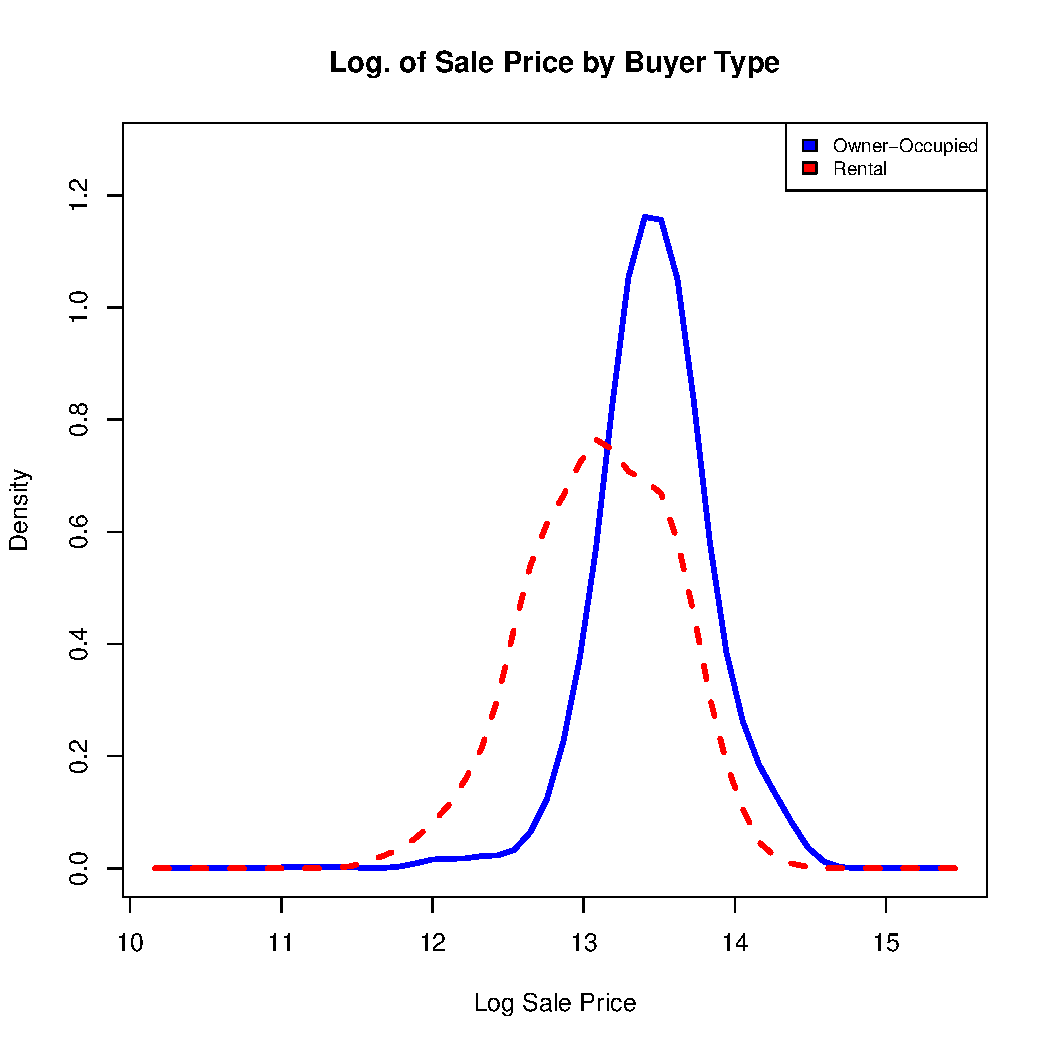
\includegraphics[scale = 0.5, keepaspectratio=true]{../Figures/log_dens_by_owner}
  \caption{Relative Density of House Log Prices of Buyer type} \label{fig:log_dens_by_owner}
\end{figure}
%
%

\bigskip
\clearpage


\begin{figure}[h!]
  \centering
  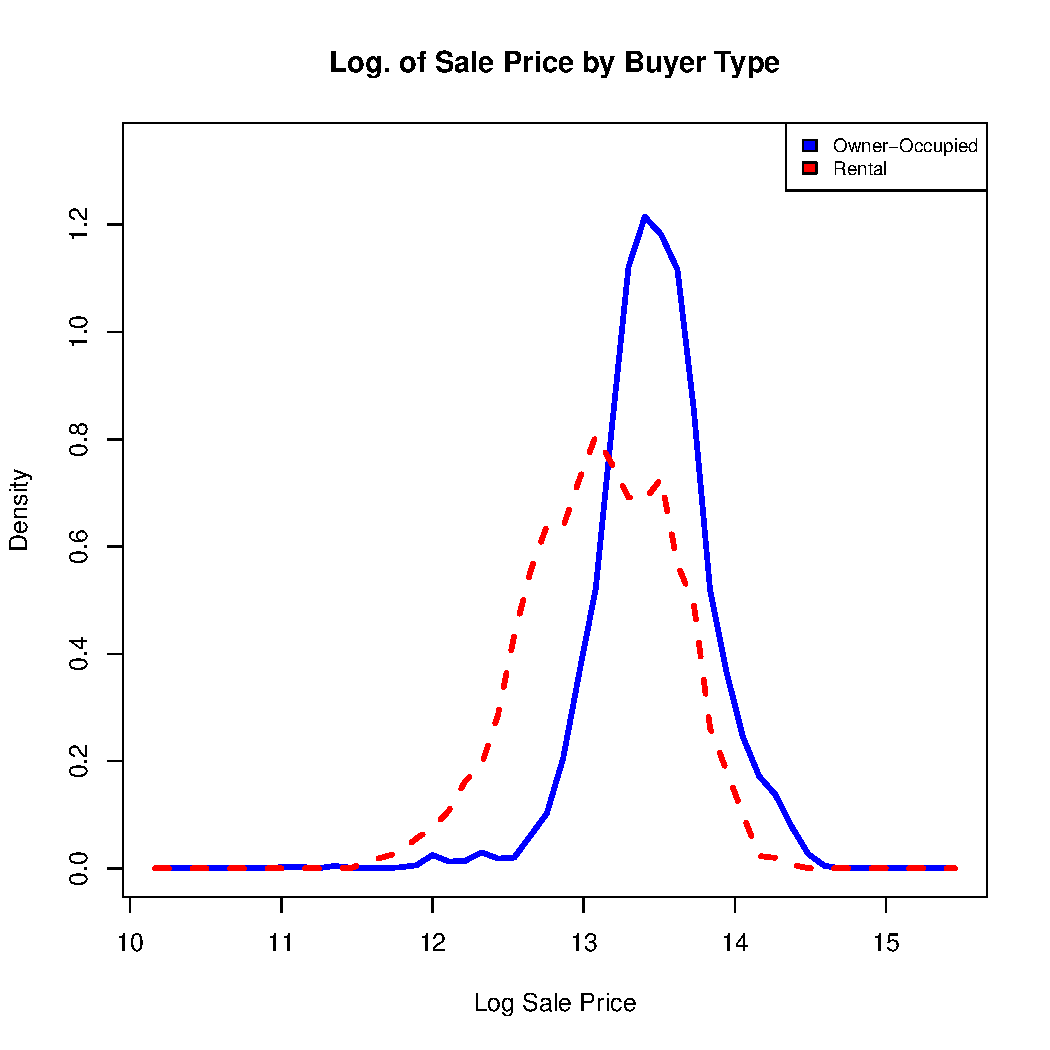
\includegraphics[scale = 0.5, keepaspectratio=true]{../Figures/log_dens_by_owner_bw}
  \caption{Relative Density of House Log Prices of Buyer type} \label{fig:log_dens_by_owner_bw}
\end{figure}


\pagebreak
When it came to adjusting the bandwidths for each Kernel-Smoothed density plot, I tried to
be careful not to over-smooth and additionally not to keep too much noise from the smaller bandwidths. Looking at the Kernel-Smoothed Density of both Owner Occupied and Rental houses.
using the natural logarithm prices, the owner-occupied houses have a bigger density than the
rental properties. Additionally, I used the bandwidth of 0.05 for owner occupied and for rental.
The rental houses prices were not as skewed as the owner-occupied ones. I do expect that the
different characteristics of homes will have different distributions relative to price and different relationships. For example, the year the house was built, or the age of the house may adversely affect the price.



%%%%%%%%%%%%%%%%%%%%%%%%%%%%%%%%%%%%%%%%
%\end{document}
%%%%%%%%%%%%%%%%%%%%%%%%%%%%%%%%%%%%%%%%


\pagebreak
\chapter{Transforming the Dependent Variable}
%\documentclass[11pt]{book}
%\usepackage{palatino}
%\usepackage{amsfonts,amsmath,amssymb}
%% \usepackage{graphicx}
%
%\usepackage{listings}
%\usepackage{textcomp}
%\usepackage{color}
%
%\definecolor{dkgreen}{rgb}{0,0.6,0}
%\definecolor{gray}{rgb}{0.5,0.5,0.5}
%\definecolor{mauve}{rgb}{0.58,0,0.82}
%
%\lstset{frame=tb,
%  language=R,
%  aboveskip=3mm,
%  belowskip=3mm,
%  showstringspaces=false,
%  columns=flexible,
%  basicstyle={\small\ttfamily},
%  numbers=none,
%  numberstyle=\tiny\color{gray},
%  keywordstyle=\color{blue},
%  commentstyle=\color{dkgreen},
%  stringstyle=\color{mauve},
%  breaklines=true,
%  breakatwhitespace=true,
%  tabsize=3
%}
%
%
%
%\ifx\pdftexversion\undefined
%    \usepackage[dvips]{graphicx}
%\else
%    \usepackage[pdftex]{graphicx}
%    \usepackage{epstopdf}
%    \epstopdfsetup{suffix=}
%\fi
%
%\usepackage{subfig}
%
%\begin{document}
%
%%%%%%%%%%%%%%%%%%%%%%%%%%%%%%%%%%%%%%%%%
%% Problem Set 3
%%%%%%%%%%%%%%%%%%%%%%%%%%%%%%%%%%%%%%%%%
%
%\pagestyle{empty}
%{\noindent\bf Spring 2023 \hfill Brandon~Parmanand}
%\vskip 16pt
%\centerline{\bf University of Central Florida}
%\centerline{\bf College of Business}
%\vskip 16pt
%\centerline{\bf QMB 6911}
%\centerline{\bf Capstone Project in Business Analytics}
%\vskip 10pt
%\centerline{\bf Solutions:  Problem Set \#3}
%\vskip 32pt
%\noindent
%
%\pagebreak
\section*{Normality of the Original and Transformed Variables}

Figure \ref{fig:qq_prices} shows a pair of Q-Q plots.
In the left panel, Figure \ref{subfig:qq_prices} shows this comparison 
for the original level of the house prices, without transformation. 
This figure shows that it deviates from the normal distribution.
In the right panel, Figure \ref{subfig:qq_log_prices} shows this comparison 
for the logarithmic transformation of house prices, without transformation. 
This figure also shows that it deviates from the normal distribution even though it is closer to it than the original level of the house prices.


\begin{figure}[!ht]
\subfloat[House Prices\label{subfig:qq_prices}]{%
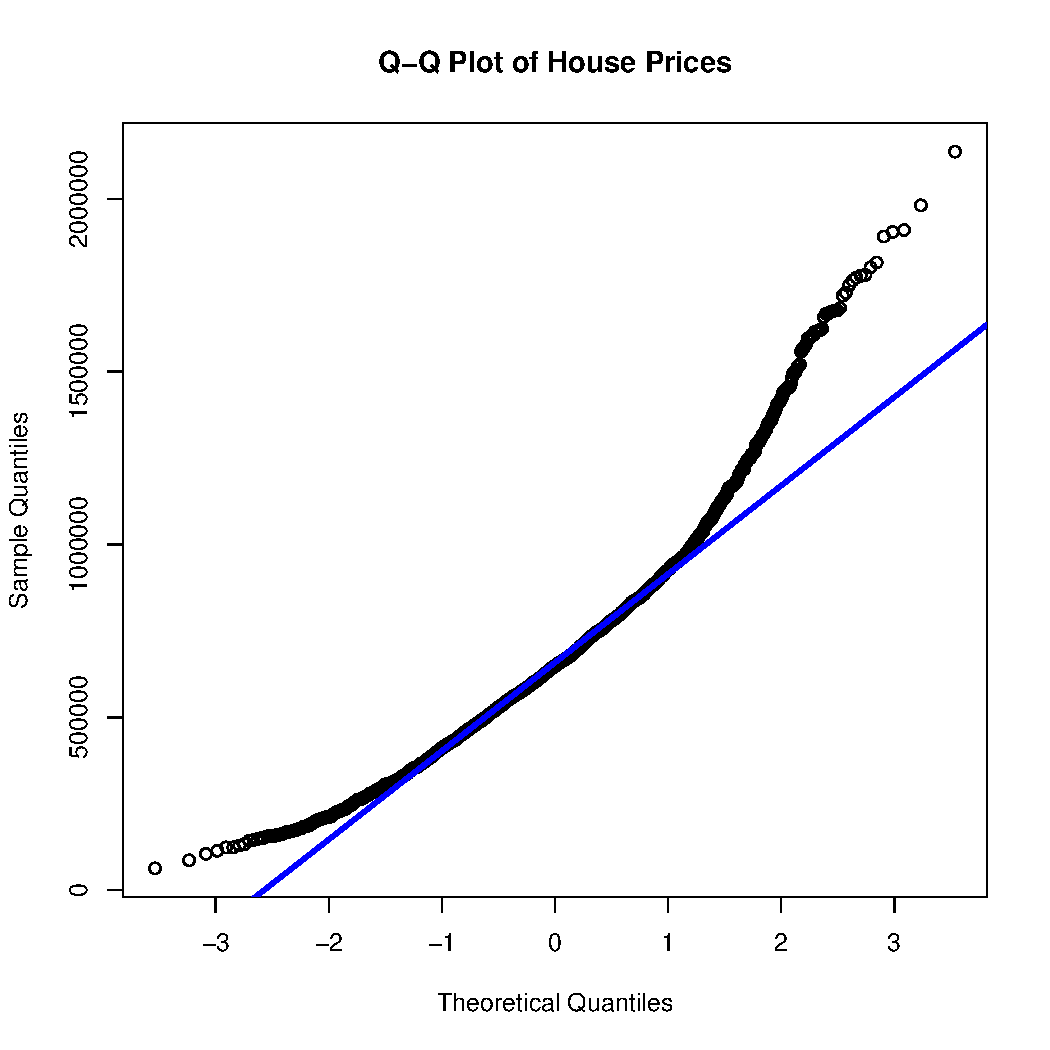
\includegraphics[width=0.5\textwidth]{../Figures/qq_prices}}
\hfill
\subfloat[Transformed House Prices\label{subfig:qq_log_prices}]{%
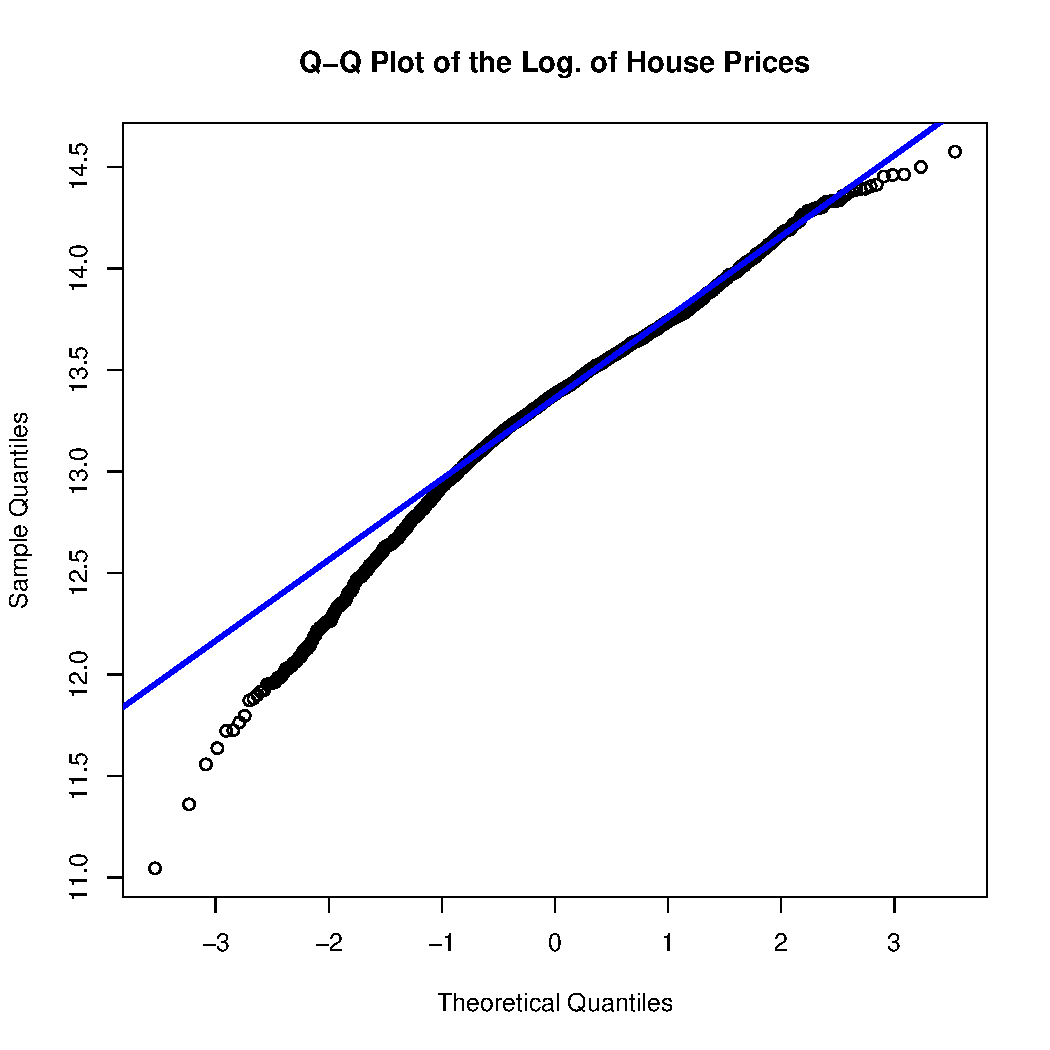
\includegraphics[width=0.5\textwidth]{../Figures/qq_log_prices}}

\caption{Q-QPlots of the Log. and Levels of House Prices}
\label{fig:qq_prices}
\end{figure}



%%%%%%%%%%%%%%%%%%%%%%%%%%%%%%%%%%%%%%%%
% Box-Cox Transformation
%%%%%%%%%%%%%%%%%%%%%%%%%%%%%%%%%%%%%%%%


\pagebreak
\section*{Box-Cox Transformation of House Prices}

The plot of this likelihood function is shown in Figure \ref{fig:box_cox_loglike_uni}.
The red points represent the values of the log-likelihood 
at the optimum $\lambda = 0.38$ and at $\lambda = 0$ and $\lambda = 1$.

\begin{figure}[h!]
  \centering
  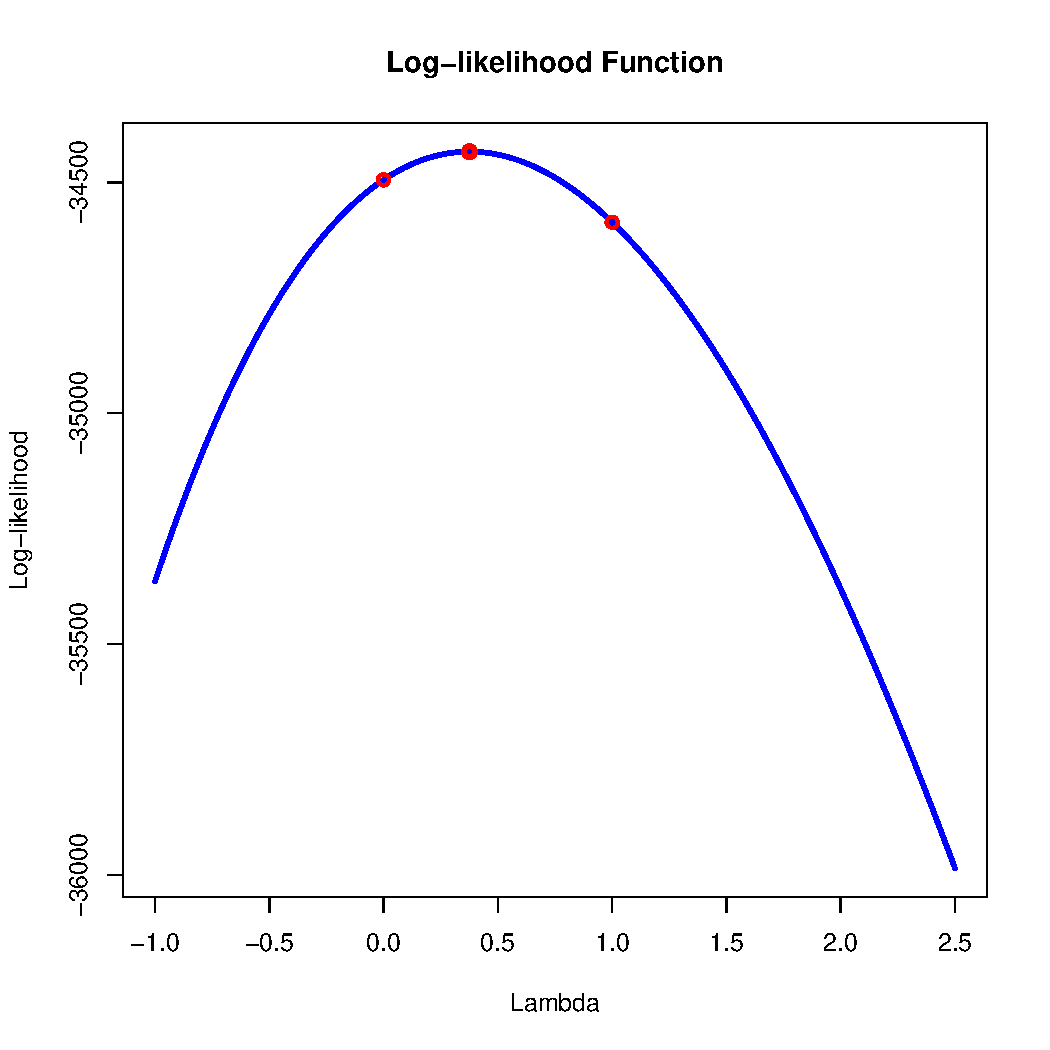
\includegraphics[scale = 0.5, keepaspectratio=true]{../Figures/box_cox_loglike_uni}
  \caption{Log-likelihood Function for Box-Cox Transformation} \label{fig:box_cox_loglike_uni}
\end{figure}


\pagebreak
\section*{Testing for an Appropriate Transformation using Likelihood Ratio}

Considering the statistical properties of these estimates
by calculating a likelihood ratio statistic. After doing the tests, 
we end up with a p-value of 0 for each so this is evidence to reject 
both and not transform with the linear or logarithmic specification.
This suggests using the transformation at the MLE but this will further 
complicate the statistical model.


\section*{Normality of the Transformed Variable}

Figure \ref{fig:qq_prices2} shows this comparison
and the panel on the right, Figure \ref{subfig:qq_boxcox}, 
shows that the quantiles of the distribution of the transformed variable
are much closer to the normal distribution but there is still a slightly notable deviation 
at $\lambda = 0.38$
Transforming at $\lambda = 0$ or $\lambda = 1$ 
was not done as the statistical test allowed us to reject those models.%
This provides statistical evidence that the prices are best modeled with the transformation
at the optimal $\lambda = 0.38$.
If other variables are added, the complexity of doing this may prove it to be not useful.


\begin{figure}[!ht]
\subfloat[Fly Reel Prices\label{subfig:qq_prices2}]{%
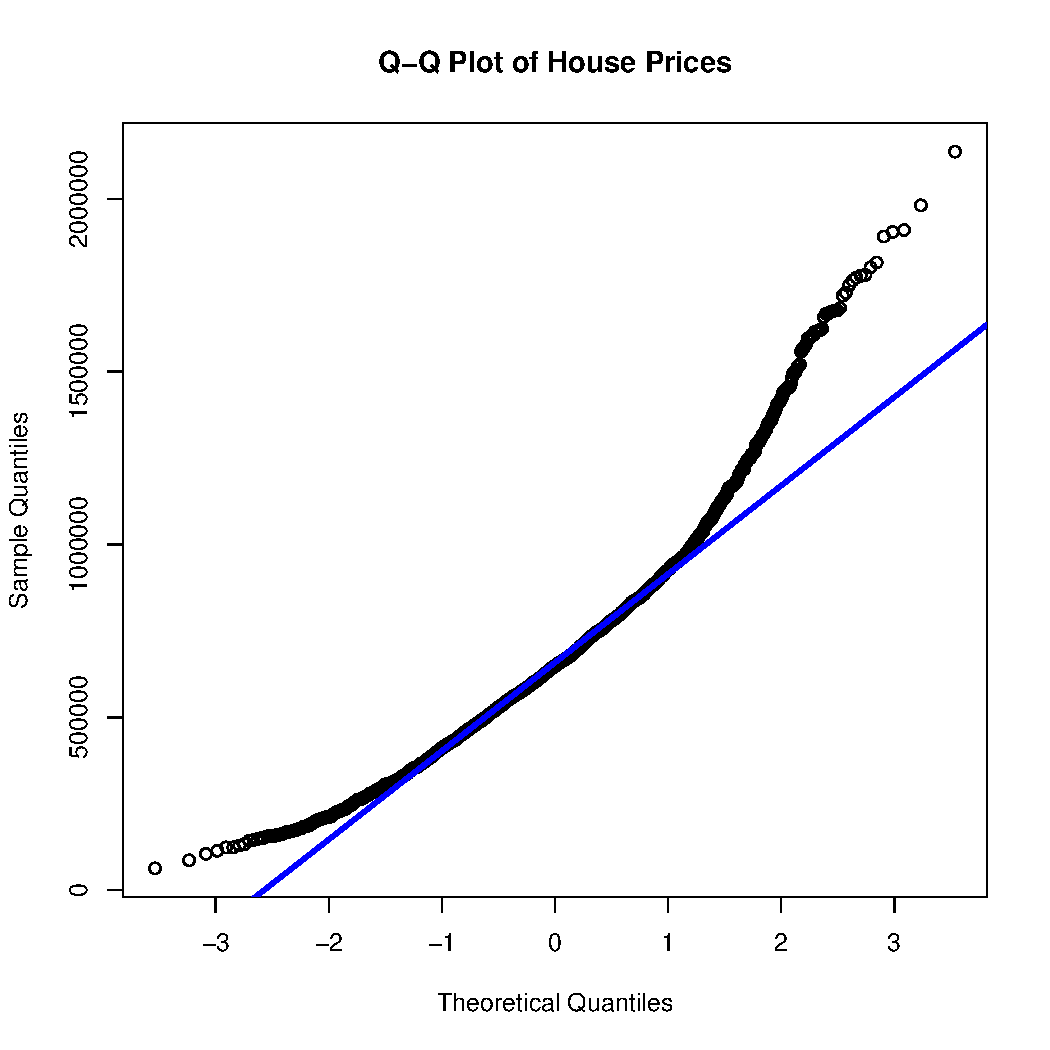
\includegraphics[width=0.5\textwidth]{../Figures/qq_prices2}}
\hfill
\subfloat[Transformed Fly Reel Prices\label{subfig:qq_boxcox}]{%
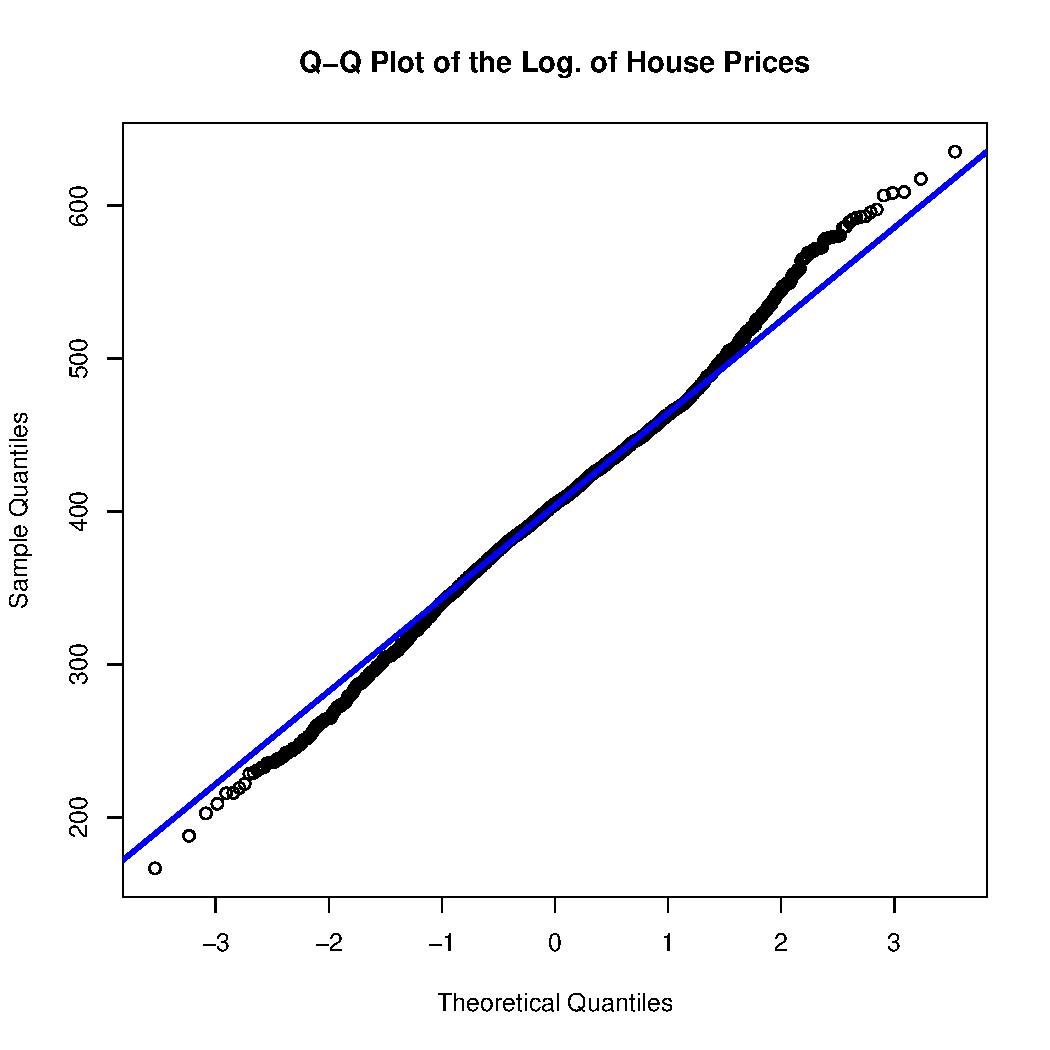
\includegraphics[width=0.5\textwidth]{../Figures/qq_boxcox}}

\caption{Q-QPlots of the Transformed Fly Reel Prices}
\label{fig:qq_prices2}
\end{figure}


\clearpage
\begin{figure}[!ht]
\subfloat[{Log. of House Prices}\label{subfig:qq_prices3}]{%
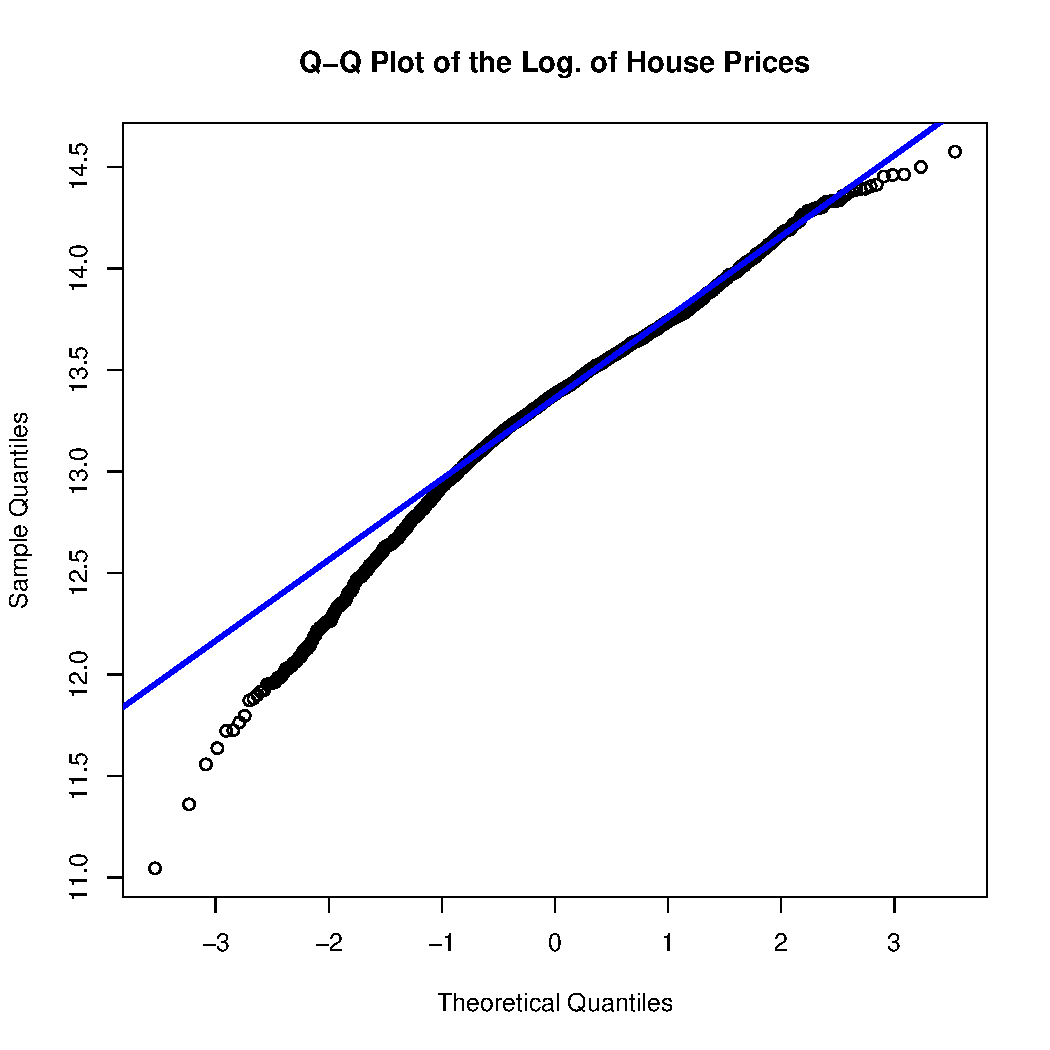
\includegraphics[width=0.5\textwidth]{../Figures/qq_log_prices}}
\hfill
\subfloat[Transformed House Prices\label{subfig:qq_boxcox_3}]{%
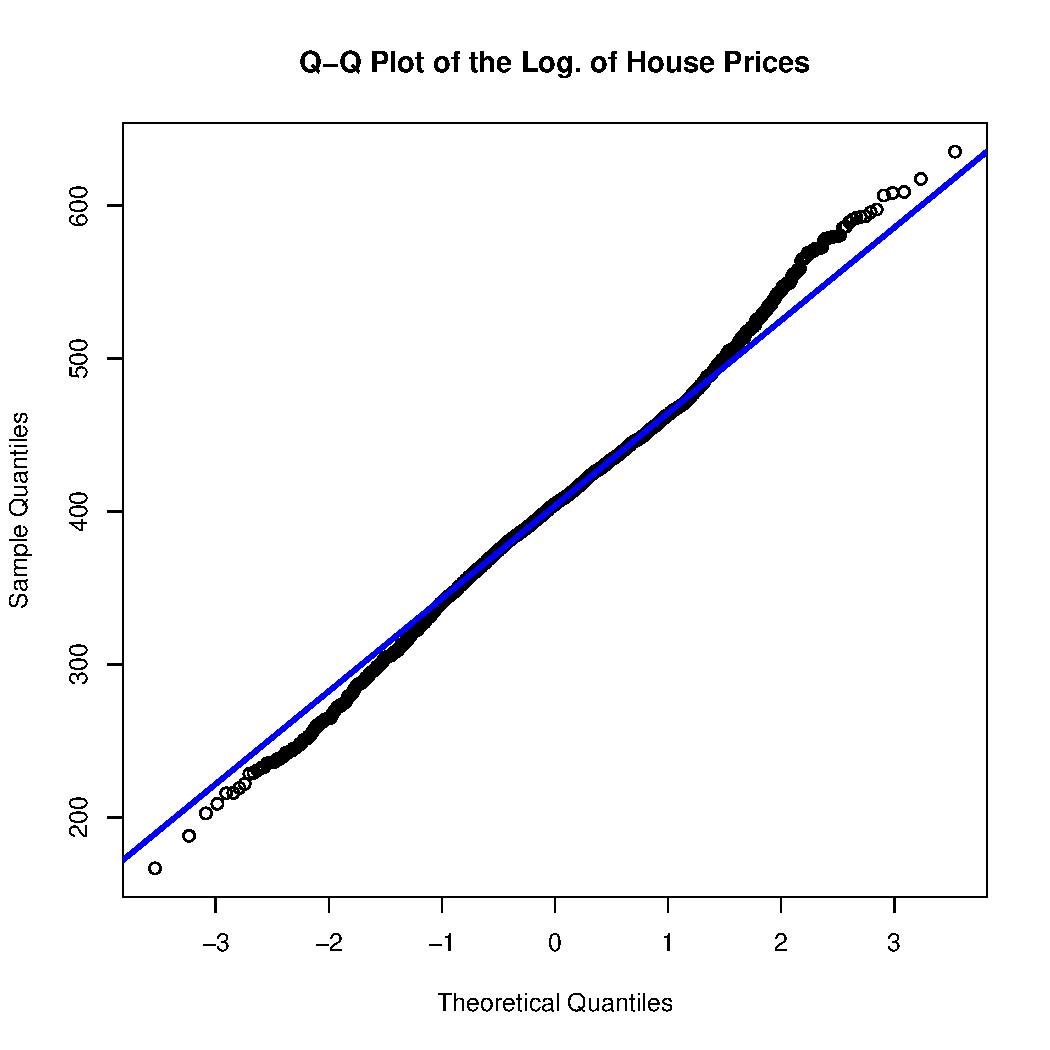
\includegraphics[width=0.5\textwidth]{../Figures/qq_boxcox}}

\caption{Q-QPlots of the Transformed House Prices}
\label{fig:qq_prices2}
\end{figure}


\clearpage

\section*{\textsf{R}  \texttt{MASS} Package for the Box-Cox Transformation}


I used the function from the \texttt{MASS} package to further my analysis.
The output is plotted in Figure \ref{fig:plot_like_MASS}. Figure \ref{subfig:plot_like_MASS_var}, 
shows that optimum is getting closer to 0 so even with the explanatory variables added%
we should take the logarithm of the prices. We get $\lambda = 0.33$ compared to 0.38 with the intial 
Box-Cox transformation. With all this info, I would not change my recommendation.
\begin{figure}[!ht]
\subfloat[ House Prices MASS\label{subfig:plot_like_MASS}]{%
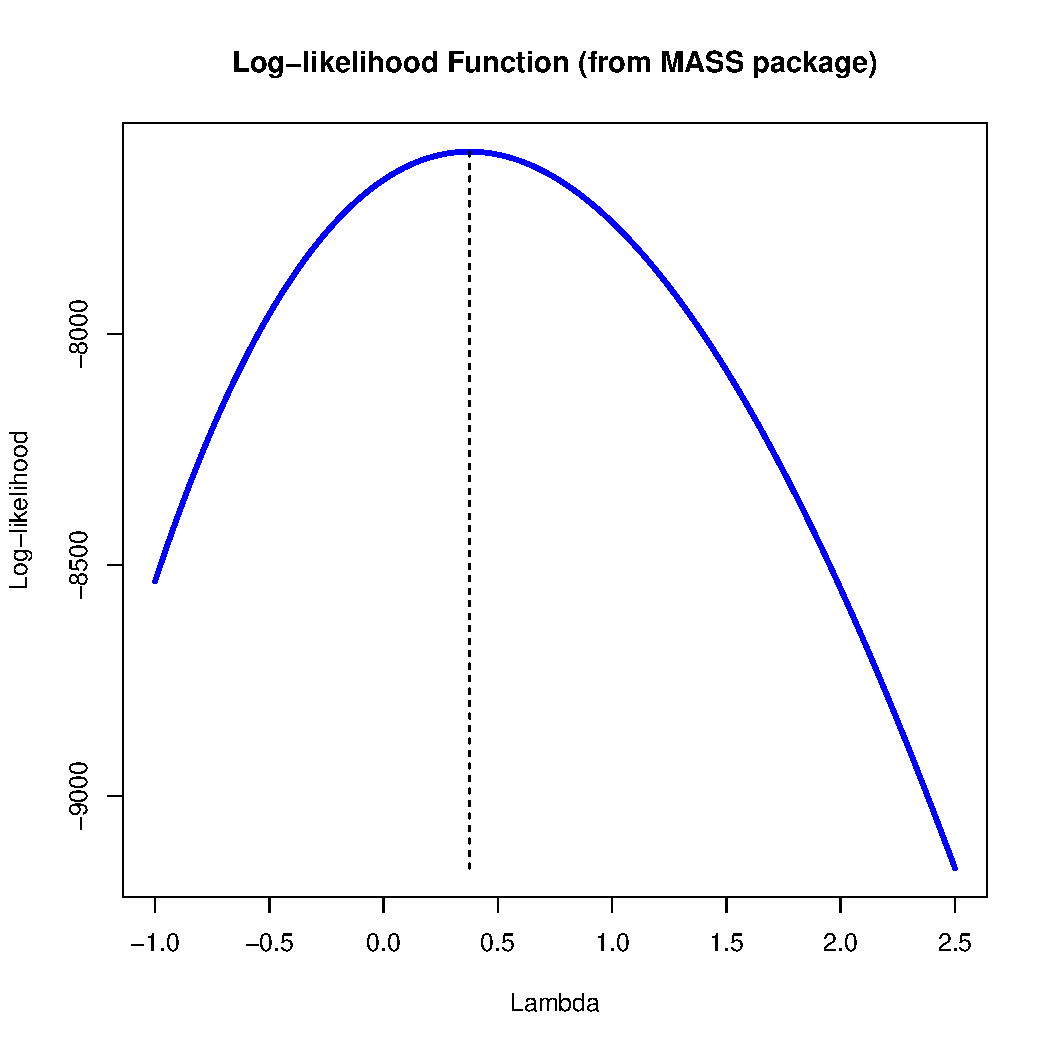
\includegraphics[width=0.5\textwidth]{../Figures/plot_like_MASS}}
\hfill
\subfloat[House Prices MASS with Vars\label{subfig:plot_like_MASS_var}]{%
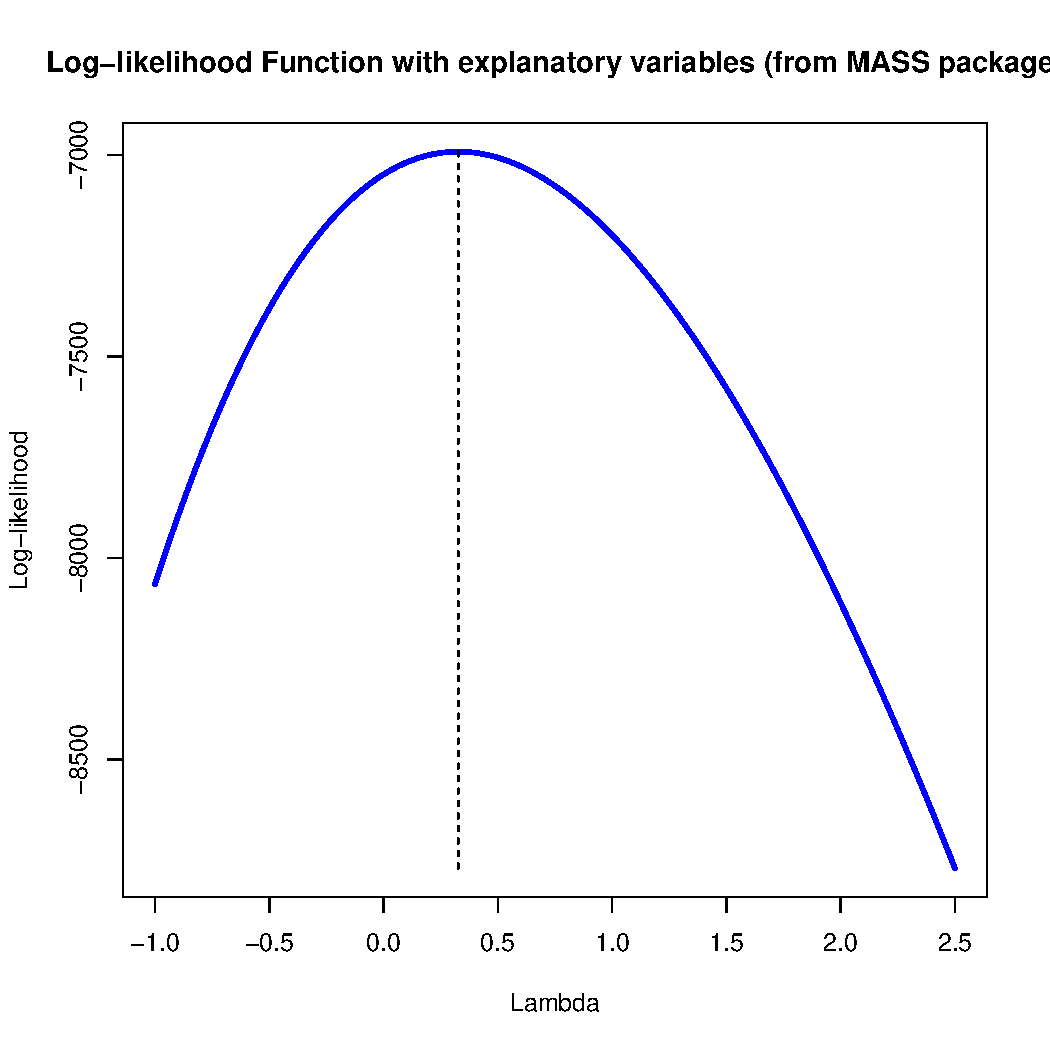
\includegraphics[width=0.5\textwidth]{../Figures/plot_like_MASS_var}}

\caption{ Transformed House Prices}
\label{fig:plot_like_MASS}
\end{figure}










%%%%%%%%%%%%%%%%%%%%%%%%%%%%%%%%%%%%%%%%
%\end{document}
%%%%%%%%%%%%%%%%%%%%%%%%%%%%%%%%%%%%%%%%


\pagebreak
\chapter{Preliminary Tabular Analysis}
%%%%%%%%%%%%%%%%%%%%%%%%%%%%%%%%%%%%%%%%%%%%%%%%%%%%%%%%%%%
%
%\documentclass[11pt]{article}
%\usepackage{fullpage}
%\usepackage{color}
%\begin{document}
%
%
%%%%%%%%%%%%%%%%%%%%%%%%%%%%%%%%%%%%%%%%%%%%%%%%%%%%%%%%%%%%%
%
%{\noindent\bf Spring 2023 \hfill Brandon Parmanand}
%\vskip 16pt
%\centerline{\bf University of Central Florida}
%\centerline{\bf College of Business }
%\vskip 16pt
%\centerline{\bf QMB 6912}
%\centerline{\bf Capstone Project in Business Analytics}
%\vskip 10pt
%\centerline{\bf Problem Set \#4}
%\vskip 32pt
%\noindent
% 
%\section{Data Description}
%% 
%\medskip
%\noindent
%I start my analysis of the data in subsets according to type of buyer, which can be Owner-Occupied and Rental, 
%calculating the summary statistics for each subset and present these 
%statistics in the \LaTeX\ tables that follow. I first created a Log. Price variable and transformed the year built column in to age by subtracting from 2021 while also doing some minor cleanup of the data.
%
%\vfill

%%%%%%%%%%%%%%%%%%%%%%%%%%%%%%%%%%%%%%%%%%%%%%%%%%%%%%%%%%%%

%\pagebreak
\section{Summary of Variables by Type of Buyer}

Table \ref{tab:summ_by_buyer} lists summary statistics for numeric variables
in separate columns for subsamples defined by the type of buyer. There is some difference with different characteristics such as the range and mean of floor space and lot size are both smaller for rentals. Rentals have higher transit scores which could make sense as renters may try to be closer to work. Prices have a larger range with owner occupied properties but the average is lower with rental properties. Age intially seems to have minimal statistical signifcance to either type of buyer.

% latex table generated in R 4.1.1 by xtable 1.8-4 package
% Thu Apr 27 14:54:27 2023
\begin{table}[ht]
\centering
\begin{tabular}{rll}
  \hline
 & Owner-Occupied & Rental \\ 
  \hline
Min. FloorSpace &  984 &  739 \\ 
  Mean FloorSpace & 1997 & 1404 \\ 
  Max. FloorSpace & 3614 & 2869 \\ 
  Min. LotSize &  2278 &  1681 \\ 
  Mean LotSize &  7361 &  5218 \\ 
  Max. LotSize & 15611 & 13432 \\ 
  Min. TransitScore &  1.000 &  1.000 \\ 
  Mean TransitScore &  4.896 &  6.375 \\ 
  Max. TransitScore & 10.000 & 10.000 \\ 
  Min. SchoolScore &  1.000 &  1.000 \\ 
  Mean SchoolScore &  6.772 &  4.251 \\ 
  Max. SchoolScore & 10.000 & 10.000 \\ 
  Min. Price &   62714 &  104624 \\ 
  Mean Price &  752405 &  546163 \\ 
  Max. Price & 2136674 & 1727860 \\ 
  Min. log\_Price & 11.05 & 11.56 \\ 
  Mean log\_Price & 13.47 & 13.10 \\ 
  Max. log\_Price & 14.57 & 14.36 \\ 
  Min. Age &  0.00 &  0.00 \\ 
  Mean Age & 11.72 & 14.08 \\ 
  Max. Age & 62.00 & 62.00 \\ 
   \hline
\end{tabular}
\caption{Summary by Type of Buyer} 
\label{tab:summ_by_buyer}
\end{table}


\pagebreak
Table \ref{tab:ind_by_buyer} lists summary statistics for categorical variables
in separate columns for subsamples defined by the type of buyer. It seems that 1 and 2 bedrooms are more within the rental buyer category than owner occupied and 1 bathrooms are most pevalent with rentals as well while 3 bathrooms are almost nonexistant in rentals.
Interestingly, it's more common that rentals have agrage while owner occupied does not. Having a patio does not show any large variances with each type of buyer, so it would be interesting to see if this has any or not any significance with the model.

% latex table generated in R 4.1.1 by xtable 1.8-4 package
% Thu Apr 27 14:54:27 2023
\begin{table}[ht]
\centering
\begin{tabular}{rrrr}
  \hline
 & Owner-Occupied & Rental & Totals \\ 
  \hline
Total & 1594 & 879 & 2473 \\ 
  1bed & 13 & 116 & 129 \\ 
  2bed & 169 & 490 & 659 \\ 
  3bed & 857 & 257 & 1114 \\ 
  4bed & 467 & 15 & 482 \\ 
  6bed & 50 & 1 & 51 \\ 
  8bed & 38 & 0 & 38 \\ 
  1bath & 463 & 575 & 1038 \\ 
  2bath & 862 & 297 & 1159 \\ 
  3bath & 269 & 7 & 276 \\ 
  Garage & 140 & 664 & 804 \\ 
  No Garage & 1454 & 215 & 1669 \\ 
  Patio & 548 & 624 & 1172 \\ 
  No Patio & 1046 & 255 & 1301 \\ 
  Security Gate & 1283 & 871 & 2154 \\ 
  No Sec Gate & 311 & 8 & 319 \\ 
  Pool & 1486 & 862 & 2348 \\ 
  No Pool & 108 & 17 & 125 \\ 
   \hline
\end{tabular}
\caption{Indicator Variables by Type of Buyer} 
\label{tab:ind_by_buyer}
\end{table}


\pagebreak
\section{Average Price by Buyer Type of Homes}

Table \ref{tab:avg_price_by_amen} lists the average price for the indicator variables such as whether there is a pool, patio, garage, or a security gate, and whether it is owner occupied or a rental buyer.  I see that no matter a rental or owner occupied, having a garage, pool, patio, or security will always have a higher average house price. Also, owner occupied buyers mean the average sales price is higher than rental average except in the case that the rental has a garage.

% latex table generated in R 4.1.1 by xtable 1.8-4 package
% Thu Apr 27 14:54:27 2023
\begin{table}[ht]
\centering
\begin{tabular}{rrrrrrrrr}
  \hline
 & No.Pool & Pool & No.Patio & Patio & No.Garage & Garage & No.Sec.Gate & Sec.Gate \\ 
  \hline
Owner-Occupied & 744768 & 857485 & 676996 & 791911 & 533482 & 773484 & 706814 & 940482 \\ 
  Rental & 546327 & 537833 & 487853 & 688852 & 460356 & 811169 & 545404 & 628819 \\ 
   \hline
\end{tabular}
\caption{Average Price of Houses by Amenities} 
\label{tab:avg_price_by_amen}
\end{table}

\medskip
Table \ref{tab:avg_price_by_bed} lists the average price for the number of bedrooms and whether it is owner occupied or a rental buyer.  Interestingly, rental properties have higher average prices for 1 bedroom and 3 bedrooms houses.

% latex table generated in R 4.1.1 by xtable 1.8-4 package
% Thu Apr 27 14:54:27 2023
\begin{table}[ht]
\centering
\begin{tabular}{rrrrrrr}
  \hline
 & 1bed & 2beds & 3beds & 4beds & 6beds & 8beds \\ 
  \hline
Owner-Occupied & 307964 & 563445 & 767302 & 717483 & 1003849 & 1507175 \\ 
  Rental & 324266 & 457981 & 804947 & 683494 & 928076 &  \\ 
   \hline
\end{tabular}
\caption{Average Price of Houses by Bedrooms} 
\label{tab:avg_price_by_bed}
\end{table}

\medskip
Table \ref{tab:avg_price_by_bath} lists the average price for the number of bathrooms and whether it is owner occupied or a rental buyer.  Rental average sales price are lower for each number of bathrooms. Notably, there is a big variance in 1 bath homes for both owner occupied and rental, with rental types being significantly lower.

% latex table generated in R 4.1.1 by xtable 1.8-4 package
% Thu Apr 27 14:54:27 2023
\begin{table}[ht]
\centering
\begin{tabular}{rrrr}
  \hline
 & 1bath & 2baths & 3baths \\ 
  \hline
Owner-Occupied & 668834 & 753718 & 892036 \\ 
  Rental & 447170 & 732732 & 761881 \\ 
   \hline
\end{tabular}
\caption{Average Price of Houses by Bathrooms} 
\label{tab:avg_price_by_bath}
\end{table}




%%%%%%%%%%%%%%%%%%%%%%%%%%%%%%%%%%%%%%%%%%%%%%%%%%%%%%%%%%%%



\pagebreak
\section{Correlation Matrices}
We plot the correlation between home prices and numerical variables. 
Table \ref{tab:correlation_num} shows the correlation 
between the log.~of house sale prices
and the numeric variables Floor Space, Lot Size, Transit Score, School score, and age.%
All variables are positively correlated with prices with the exception of Age. Transit score is also not heavily correlated with the price with a coefficient of 0.120.


% \input{../Tables/correlation_ind}
\input{../Tables/correlation_num}

We plot the correlation between home prices and categorixal variables. 
Table \ref{tab:correlation_ind} shows the correlation 
between the log.~of house sale prices
and the categorical variables including Number of Beds, Number of Baths, whether it has a garage, pool, patio, and security gate.
All variables are positively correlated with prices. Whether it has a pool is not heavily correlated with the price with a coefficient of 0.09.


\input{../Tables/correlation_ind}





%\end{document}

%%%%%%%%%%%%%%%%%%%%%%%%%%%%%%%%%%%%%%%%%%%%%%%%%%%%%%%%%%%%


\pagebreak
\chapter{Preliminary Graphical Analysis}
%\documentclass[11pt]{book}
%\usepackage{palatino}
%\usepackage{amsfonts,amsmath,amssymb}
%% \usepackage{graphicx}
%
%
%\ifx\pdftexversion\undefined
%    \usepackage[dvips]{graphicx}
%\else
%    \usepackage[pdftex]{graphicx}
%    \usepackage{epstopdf}
%    \epstopdfsetup{suffix=}
%\fi
%
%\usepackage{color}
%
%\begin{document}
%
%%%%%%%%%%%%%%%%%%%%%%%%%%%%%%%%%%%%%%%%%
%% Problem Set 5
%%%%%%%%%%%%%%%%%%%%%%%%%%%%%%%%%%%%%%%%%
%
%\pagestyle{empty}
%{\noindent\bf Spring 2023 \hfill Brandon~Parmanand}
%\vskip 16pt
%\centerline{\bf University of Central Florida}
%\centerline{\bf College of Business}
%\vskip 16pt
%\centerline{\bf QMB 6911}
%\centerline{\bf Capstone Project in Business Analytics}
%\vskip 10pt
%\centerline{\bf Solutions:  Problem Set \#5}
%\vskip 32pt
%\noindent
%
%
%
%
%\section{Histogram and Density of Log. {\color{red} Fly Reel} Prices}
%
%To begin visually analyzing the data, 
%include plots of the density that were created from last milestones.
%
%\subsection{All Houses Together}
%
%Start with the log of prices because prices were skewed.
%Figure \ref{fig:hist_dens_log_price} is
%a histogram of the logarithm of house prices, 
%along with a rug plot and a kernel density estimate. 
%%
%\begin{figure}[h!]
%  \centering
%  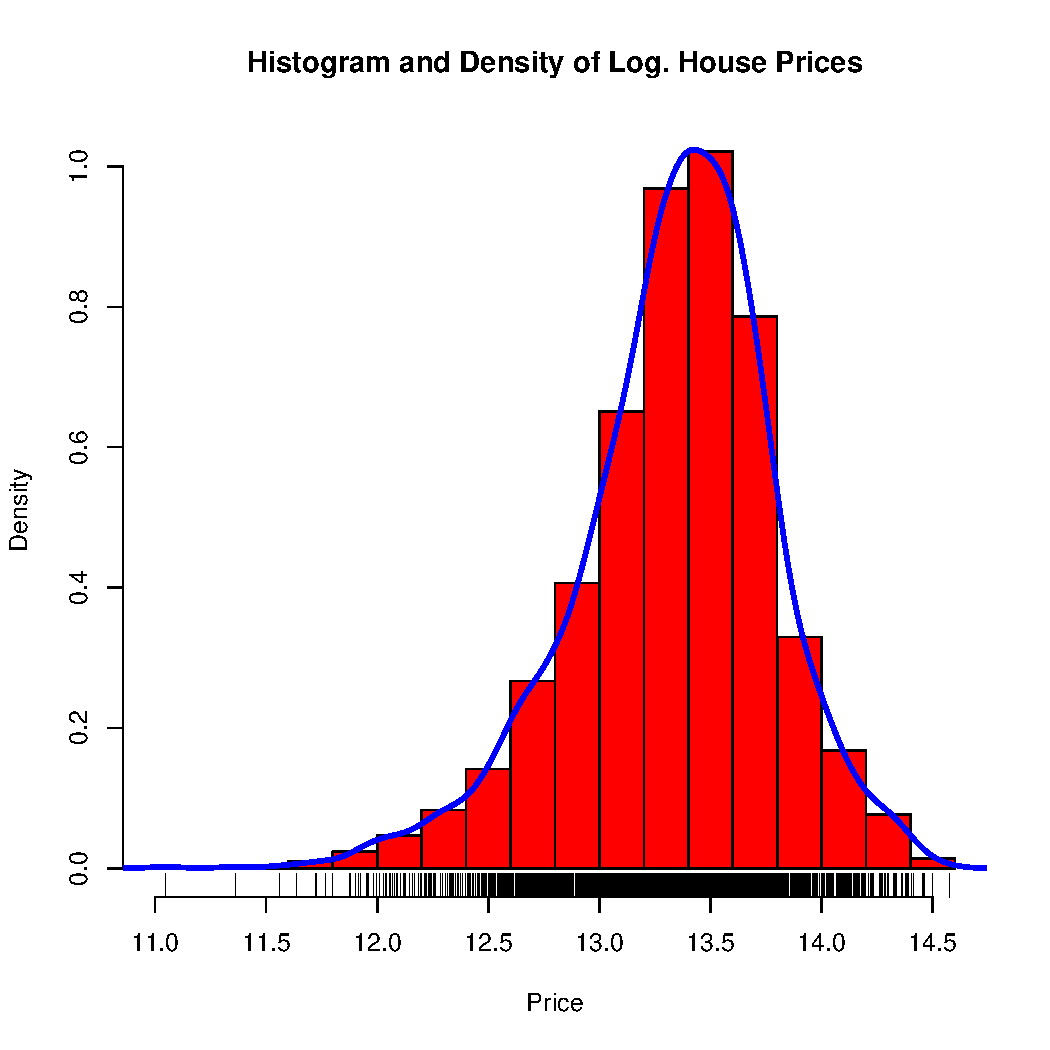
\includegraphics[scale = 0.5, keepaspectratio=true]{../Figures/hist_dens_log_price}
%  \caption{Relative Histogram of Fly Reel Prices} \label{fig:hist_dens_log_price}
%\end{figure}
%% 
%After taking logs, we can see that the distribution is
%approximately symmetric, now with a slight skew to the left. 
% 
%
%
%\clearpage
%\pagebreak
%\subsection{Comparison By Type of Buyer}
%
%Now we investigate the prices of houses that are owner occupied 
%compared to rental homes.
%Figure \ref{fig:dens_by_TypeOfBuyer} shows the 
%kernel density estimate of the prices of 
%owner occupied houses in blue
%and rental houses in red.
%% 
%I observed more variability in the prices of rental houses. 
%Owner-occupied houses are in the higher price range compared to rentals.
%
%{\color{red} As I mentioned earlier, the default bandwidth makes this very smooth, 
%so that the distributions look artificially normal or mixed normal.
%Also, this feature could be applied to other variables for more insight.}
%
%
%
%\begin{figure}[h!]
%  \centering
%  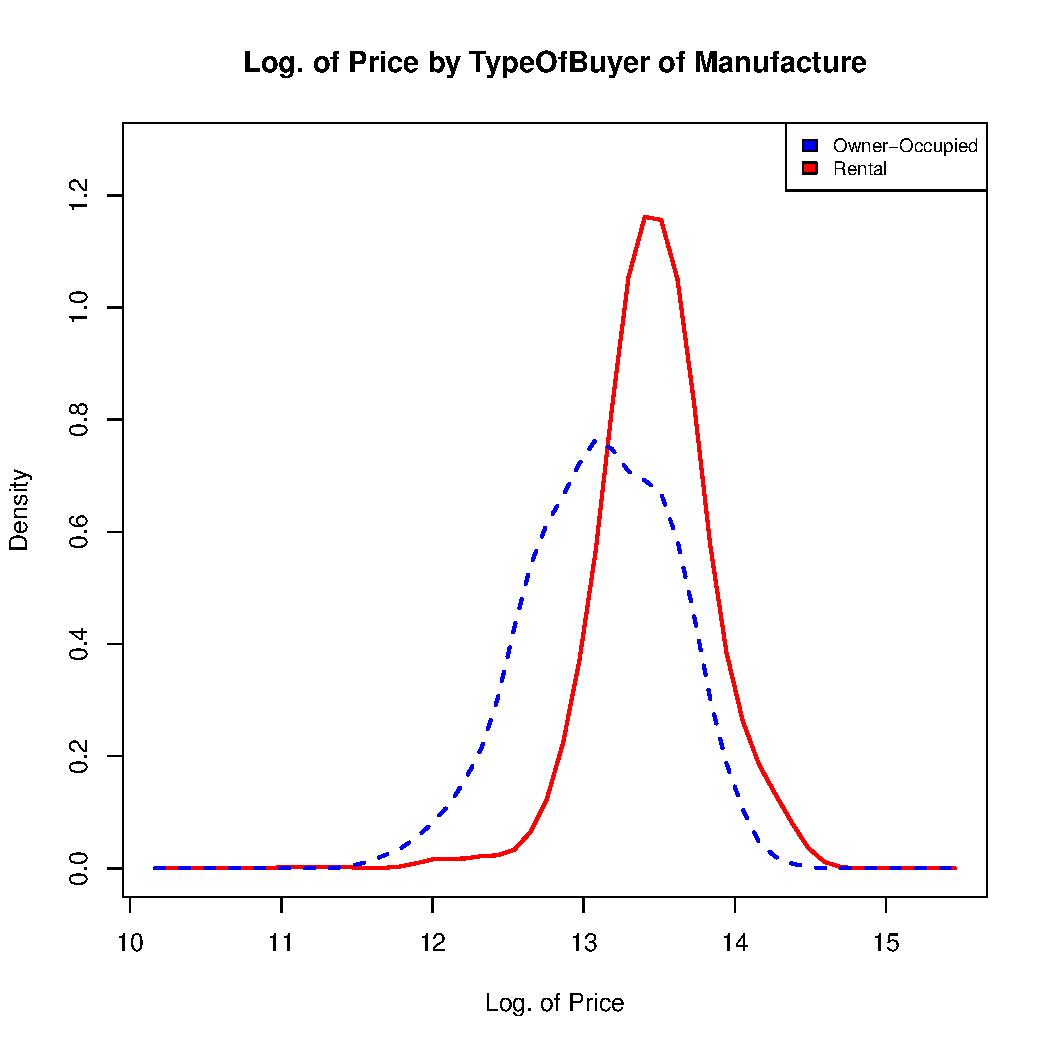
\includegraphics[scale = 0.5, keepaspectratio=true]{../Figures/dens_by_TypeOfBuyer}
%  \caption{Densities of Log.House Prices by Country of Manufacture} \label{fig:dens_by_TypeOfBuyer}
%\end{figure}
%
%
%\clearpage
%\pagebreak

I observed more variability in the prices of rental houses. 
Owner-occupied houses are in the higher price range compared to rentals.

\section*{Scatterplot Matrices}


\subsection*{Scatterplots of Numeric Variables}

Figure \ref{fig:slpom_num_only} depicts a matrix of scatterplots
of the numeric variables in the dataset.


\begin{figure}[h!]
  \centering
  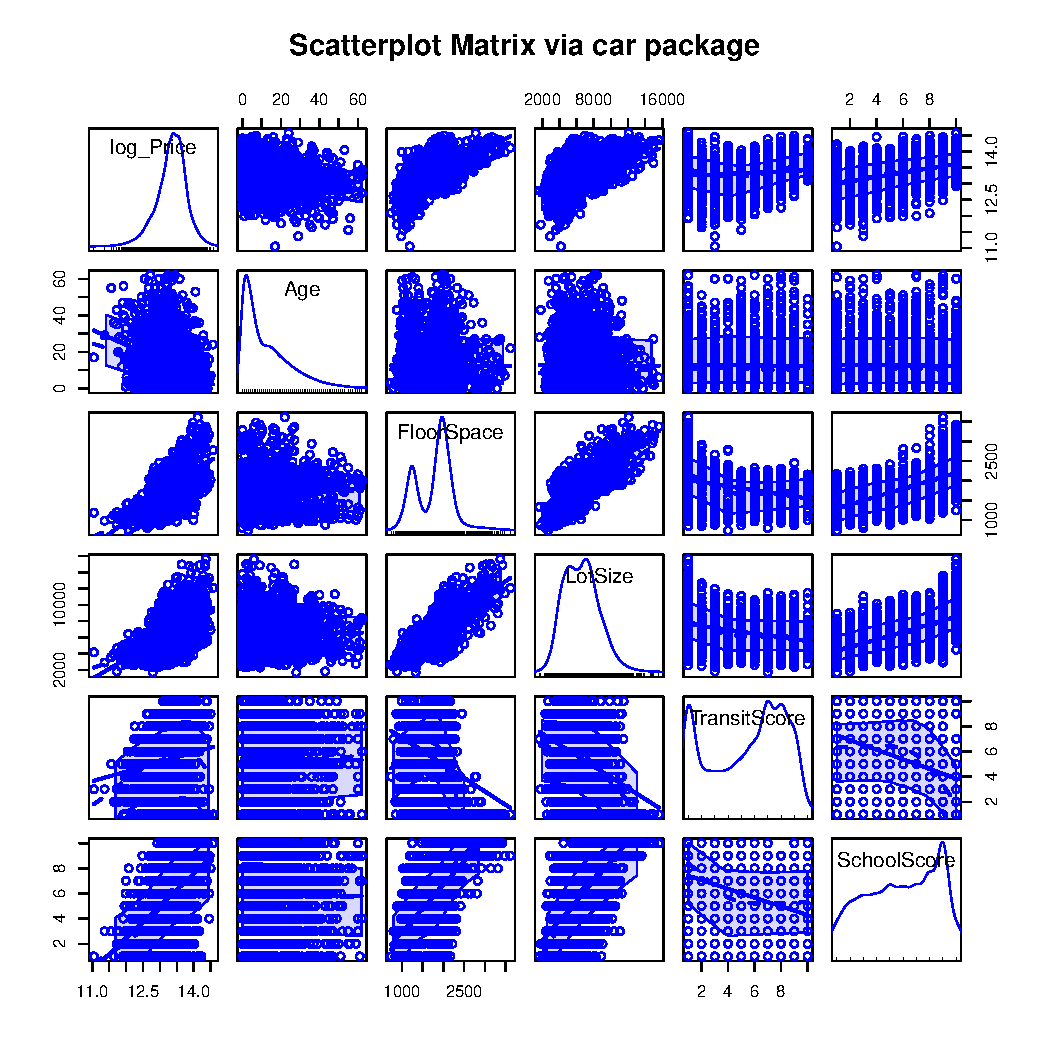
\includegraphics[scale = 0.5, keepaspectratio=true]{../Figures/slpom_num_only}
  \caption{Scatterplots of Numeric Variables} \label{fig:slpom_num_only}
\end{figure}


\pagebreak
\subsection*{Scatterplots with Categorical Variables}

Figure \ref{fig:slpom_by_buyer} depicts a matrix of scatterplots
of some categorical variables in the dataset.

\begin{figure}[h!]
  \centering
  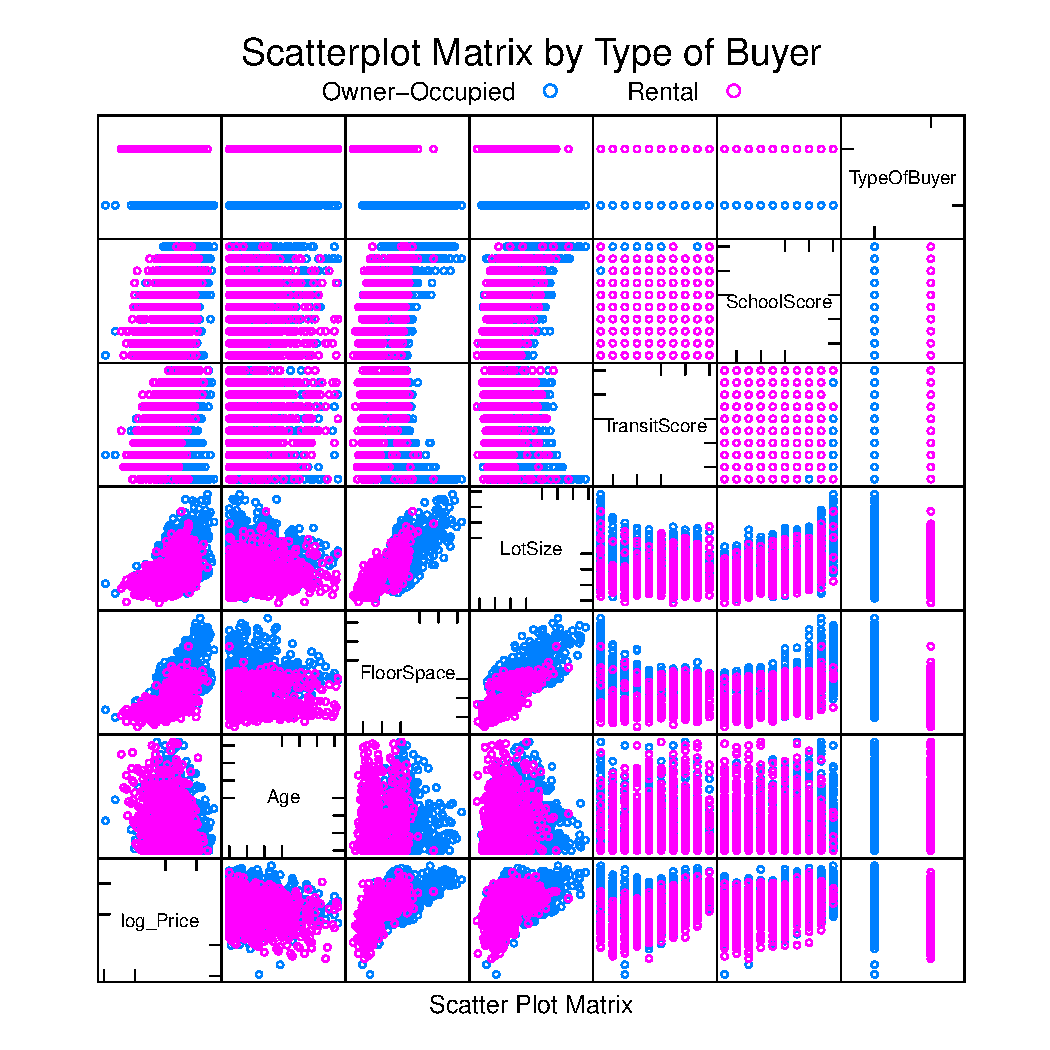
\includegraphics[scale = 0.5, keepaspectratio=true]{../Figures/slpom_by_buyer}
  \caption{Scatterplots with Categorical Variables Colored by Type of Buyer} \label{fig:slpom_by_buyer}
\end{figure}


\pagebreak

\subsection*{Spinograms by Type of Buyer}

Figure \ref{fig:buyer_and_EnclPatio_sales} depicts a spinogram
of the type of buyer and whether it has an enclosed patio.

\begin{figure}[h!]
  \centering
  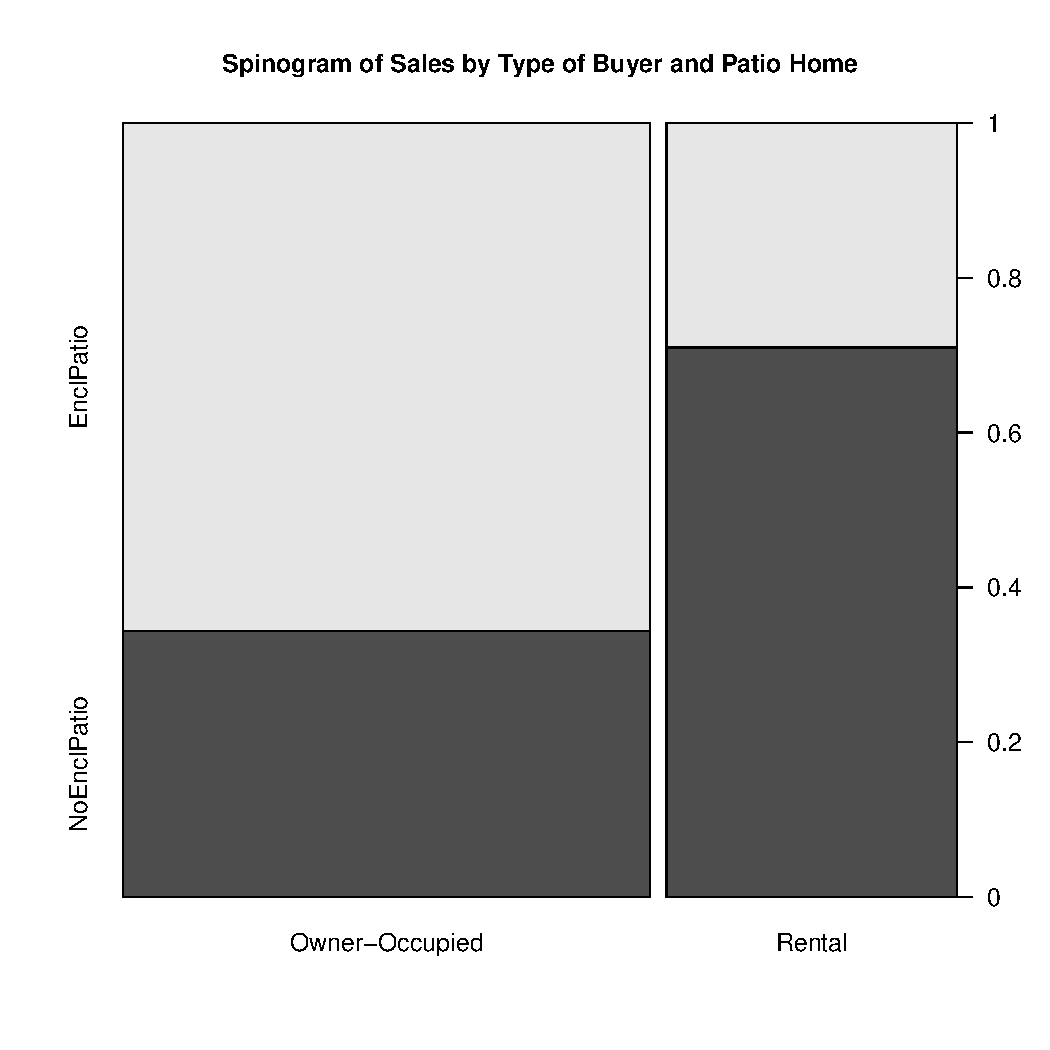
\includegraphics[scale = 0.5, keepaspectratio=true]{../Figures/buyer_and_EnclPatio_sales}
  \caption{Scatterplots by Type of Buyer and Patio} \label{fig:buyer_and_EnclPatio_sales}
\end{figure}

\pagebreak

Figure \ref{fig:buyer_and_SecGate_sales} depicts a spinogram
of the type of buyer and whether it has a security gate.

\begin{figure}[h!]
  \centering
  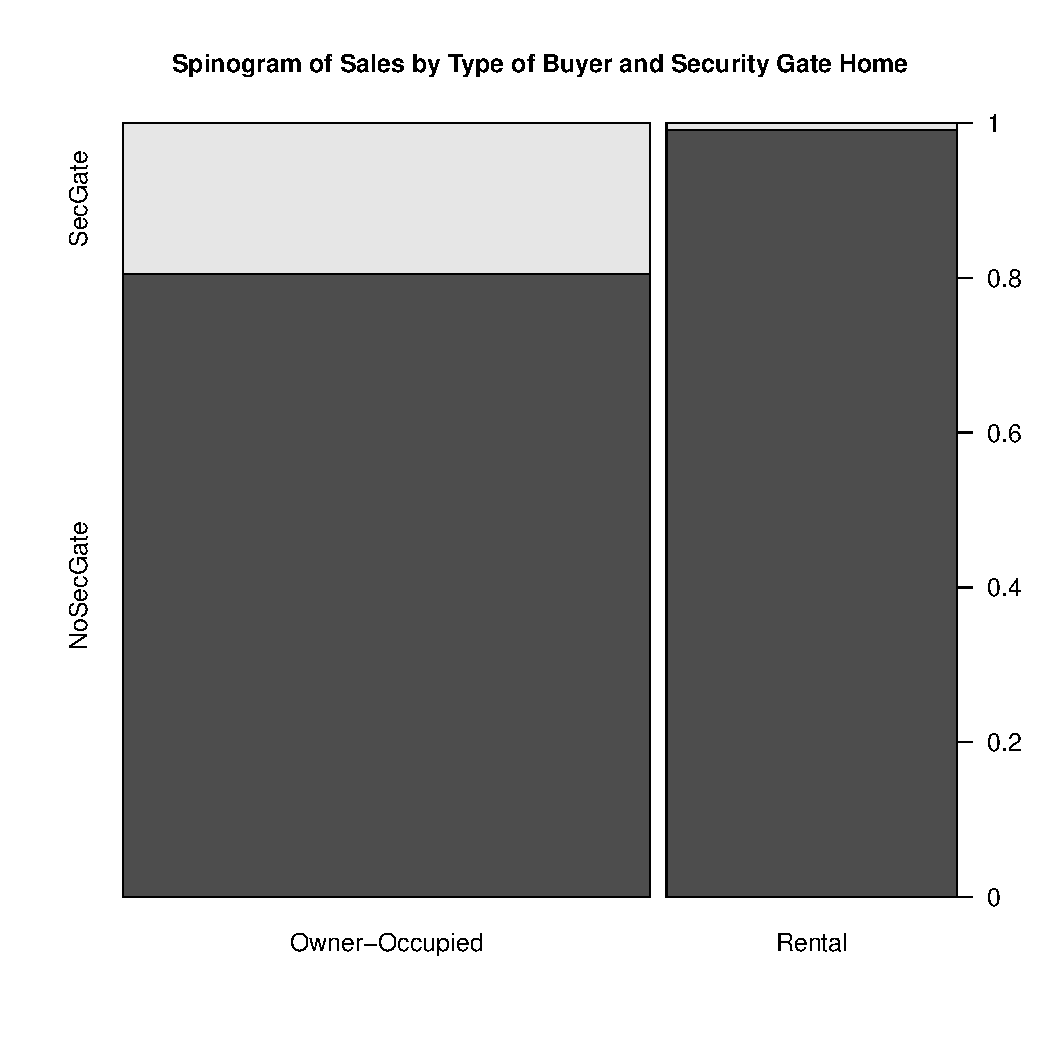
\includegraphics[scale = 0.5, keepaspectratio=true]{../Figures/buyer_and_SecGate_sales}
  \caption{Scatterplots by Type of Buyer and Securty Gate} \label{fig:buyer_and_SecGate_sales}
\end{figure}

\pagebreak

Figure \ref{fig:buyer_and_pool_sales} depicts a spinogram
of the type of buyer and whether it has an pool.

\begin{figure}[h!]
  \centering
  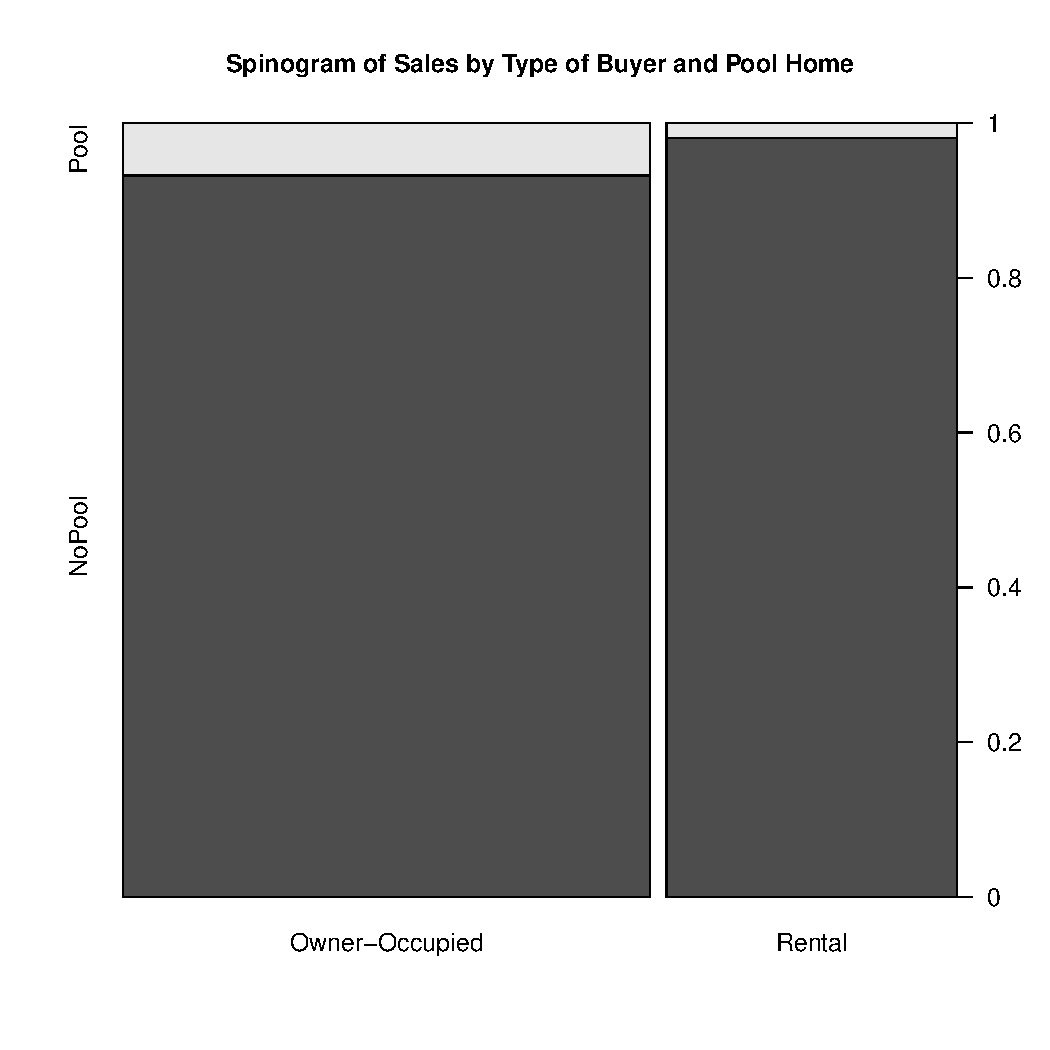
\includegraphics[scale = 0.5, keepaspectratio=true]{../Figures/buyer_and_pool_sales}
  \caption{Scatterplots by Type of Buyer and Pool} \label{fig:buyer_and_pool_sales}
\end{figure}

\pagebreak
\subsection*{Dot Chart byType of Buyer and Average Price}

Figure \ref{fig:dotchart_beds_TypeOfBuyer} depicts a dot chart
showing the average prices by number of bedrooms and type of buyer



\begin{figure}[h!]
  \centering
  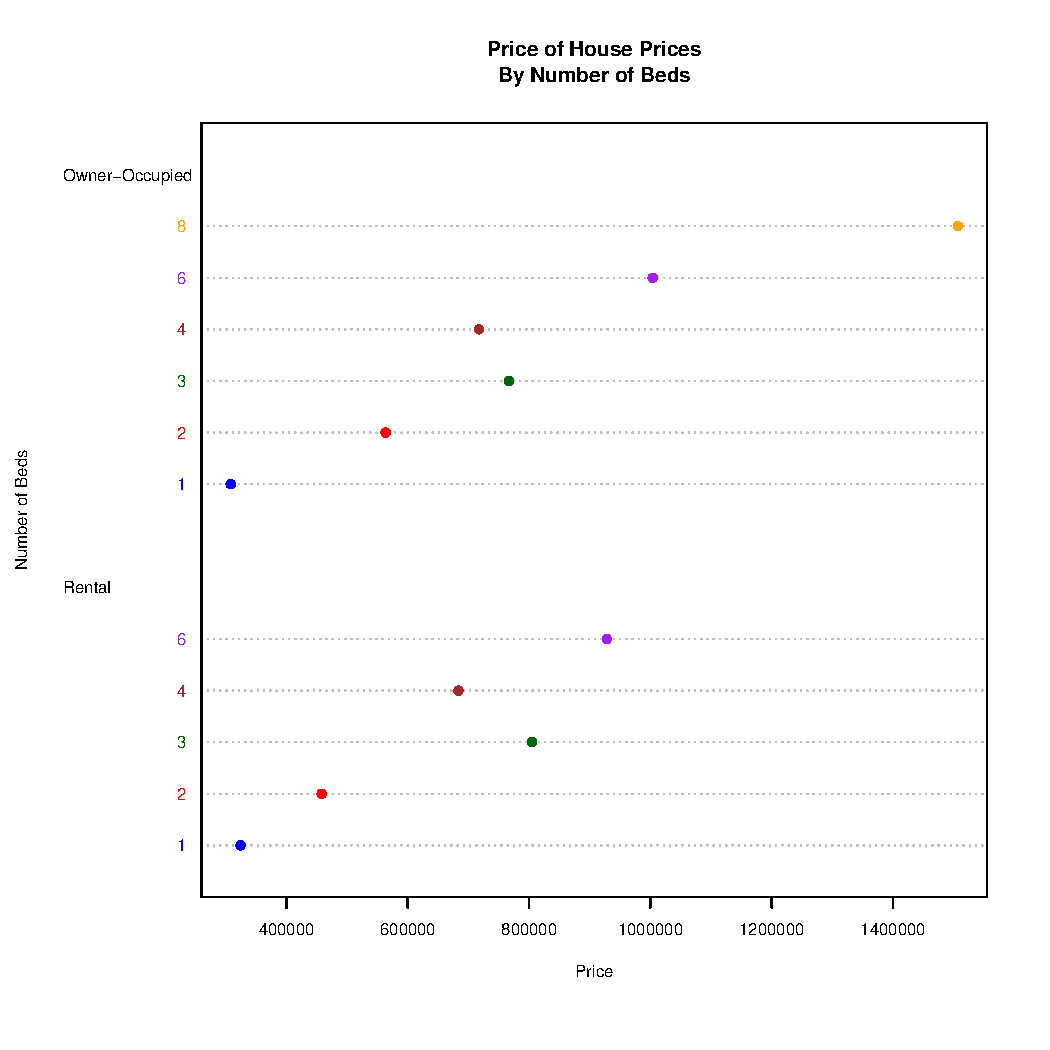
\includegraphics[scale = 0.5, keepaspectratio=true]{../Figures/dotchart_beds_TypeOfBuyer}
  \caption{Average Prices by Number of Bedrooms and Type of Buyer} \label{fig:dotchart_beds_TypeOfBuyer}
\end{figure}

\pagebreak
Figure \ref{fig:dotchart_baths_TypeOfBuyer} depicts a dot chart
showing the average prices by number of bedrooms and type of buyer


\begin{figure}[h!]
  \centering
  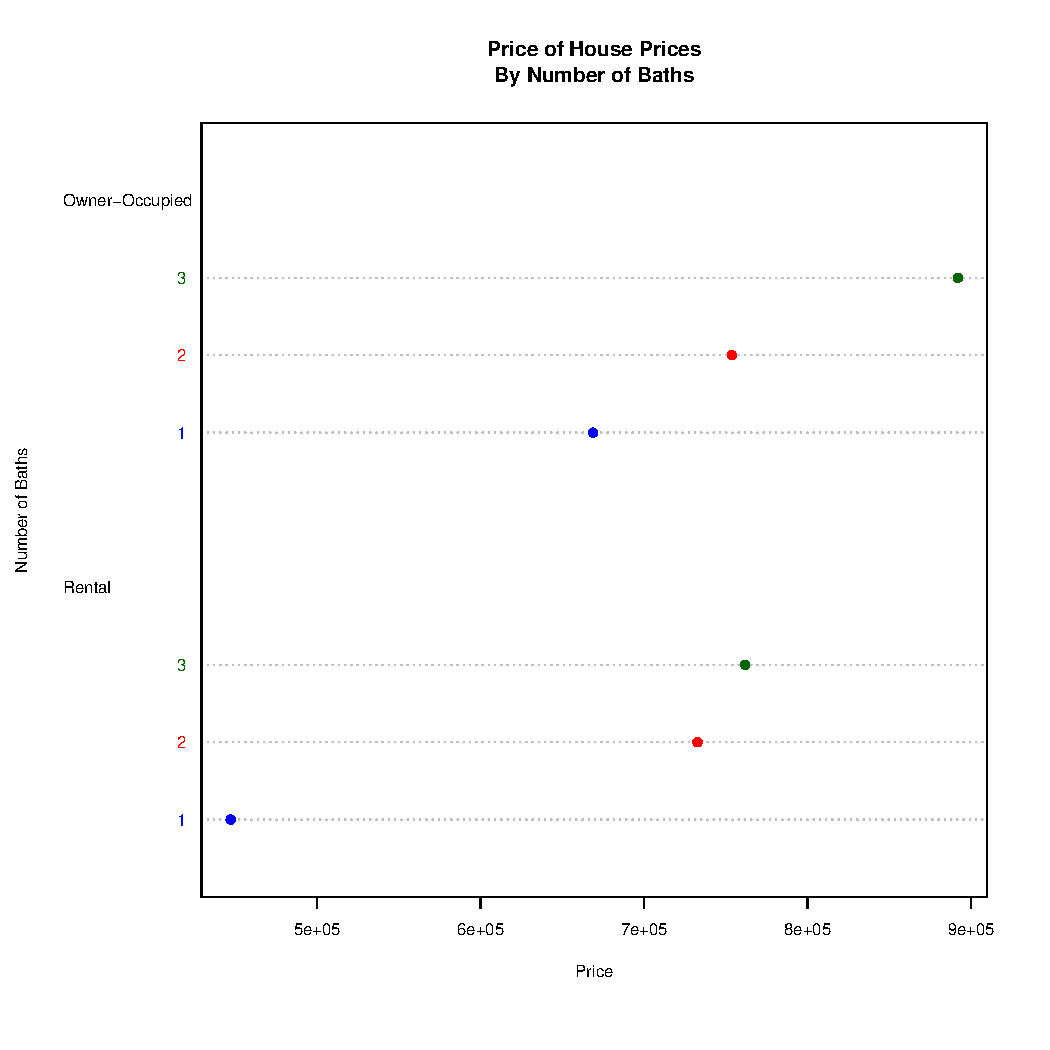
\includegraphics[scale = 0.5, keepaspectratio=true]{../Figures/dotchart_baths_TypeOfBuyer}
  \caption{Average Prices by Number of Bathrooms and Type of Buyer} \label{fig:dotchart_baths_TypeOfBuyer}
\end{figure}

\pagebreak
\subsection*{Summary}
Looking at the dot charts for number of bedrooms, we see that as the number of bedrooms increase,
the average price increases for both owner occupied and rental houses with the exception of 3 and 4 bedrooms where 
4 bedrooms average price is lower than 3 bedrooms. We also see that as the number of bathrooms increase, so does the average price
for both types of buyers. 1 bathroom rentals seem significantly cheaper than 1 bathroom owner occupied. The number of beds and nunber of baths 
is something I would like to keep in the regression model. Additionally, looking at whether it has a garage or not is also seems like a good variable to keep in the model.
Having a patio and secuirty gates may be two variables that need to be looked at more to see if they are suitable to be in the model. 


%%%%%%%%%%%%%%%%%%%%%%%%%%%%%%%%%%%%%%%%
%\end{document}
%%%%%%%%%%%%%%%%%%%%%%%%%%%%%%%%%%%%%%%%


\pagebreak
\chapter{Regression Modelling with Hedonic Price Theory}
%\documentclass[11pt]{paper}
%\usepackage{palatino}
%\usepackage{amsfonts,amsmath,amssymb}
%% \usepackage{graphicx}
%
%\usepackage{listings}
%\usepackage{textcomp}
%\usepackage{color}
%
%\definecolor{dkgreen}{rgb}{0,0.6,0}
%\definecolor{gray}{rgb}{0.5,0.5,0.5}
%\definecolor{mauve}{rgb}{0.58,0,0.82}
%
%\lstset{frame=tb,
%  language=R,
%  aboveskip=3mm,
%  belowskip=3mm,
%  showstringspaces=false,
%  columns=flexible,
%  basicstyle={\small\ttfamily},
%  numbers=none,
%  numberstyle=\tiny\color{gray},
%  keywordstyle=\color{blue},
%  commentstyle=\color{dkgreen},
%  stringstyle=\color{mauve},
%  breaklines=true,
%  breakatwhitespace=true,
%  tabsize=3
%}
%
%
%
%\ifx\pdftexversion\undefined
%    \usepackage[dvips]{graphicx}
%\else
%    \usepackage[pdftex]{graphicx}
%    \usepackage{epstopdf}
%    \epstopdfsetup{suffix=}
%\fi
%
%\usepackage{subfig}
%
%\begin{document}
%
%%%%%%%%%%%%%%%%%%%%%%%%%%%%%%%%%%%%%%%%%
%% Problem Set 6
%%%%%%%%%%%%%%%%%%%%%%%%%%%%%%%%%%%%%%%%%
%
%\pagestyle{empty}
%{\noindent\bf Spring 2023 \hfill Brandon~Parmanand}
%\vskip 16pt
%\centerline{\bf University of Central Florida}
%\centerline{\bf College of Business}
%\vskip 16pt
%\centerline{\bf QMB 6911}
%\centerline{\bf Capstone Project in Business Analytics}
%\vskip 10pt
%\centerline{\bf Solutions:  Problem Set \#6}
%\vskip 32pt
%\noindent
%
%\section{Data Description}
%
%This analysis follows the script \texttt{PS6.R} to produce a more accurate model for House prices with the data from \texttt{HomeSales.dat} in the \texttt{Data} folder. 
%
%
I will first estimate a model with the entire sampeles, including both rental and owner occupied. Then I will consider exclusions of insignificant variables from the full model. 
This approach allows for exclusion of possibly irrelevant variables and avoids excluding any relevant variables. 


%%%%%%%%%%%%%%%%%%%%%%%%%%%%%%%%%%%%%%%%
% Choosing the Dependent Variable
%%%%%%%%%%%%%%%%%%%%%%%%%%%%%%%%%%%%%%%%


\pagebreak
\section{Choosing the Dependent Variable}

Before we begin, I review the evidence for the suitability of the 
dependent variable without transformation
and compare that with the logarithmic transformation. 
Although, in this case, this decision is fairly clearly made by plotting the dependent variable alone, 
in many cases, the decision is not so clear and other forms
of evidence can be considered once building a model. 


\subsection{Univariate Analysis}

Figure \ref{fig:hist_price} shows a histogram of home prices.
This is a skewed distribution, which might influence the
estimates of parameters in the model so I will plot a histogram of the log of home prices.


\begin{figure}[h!]
  \centering
  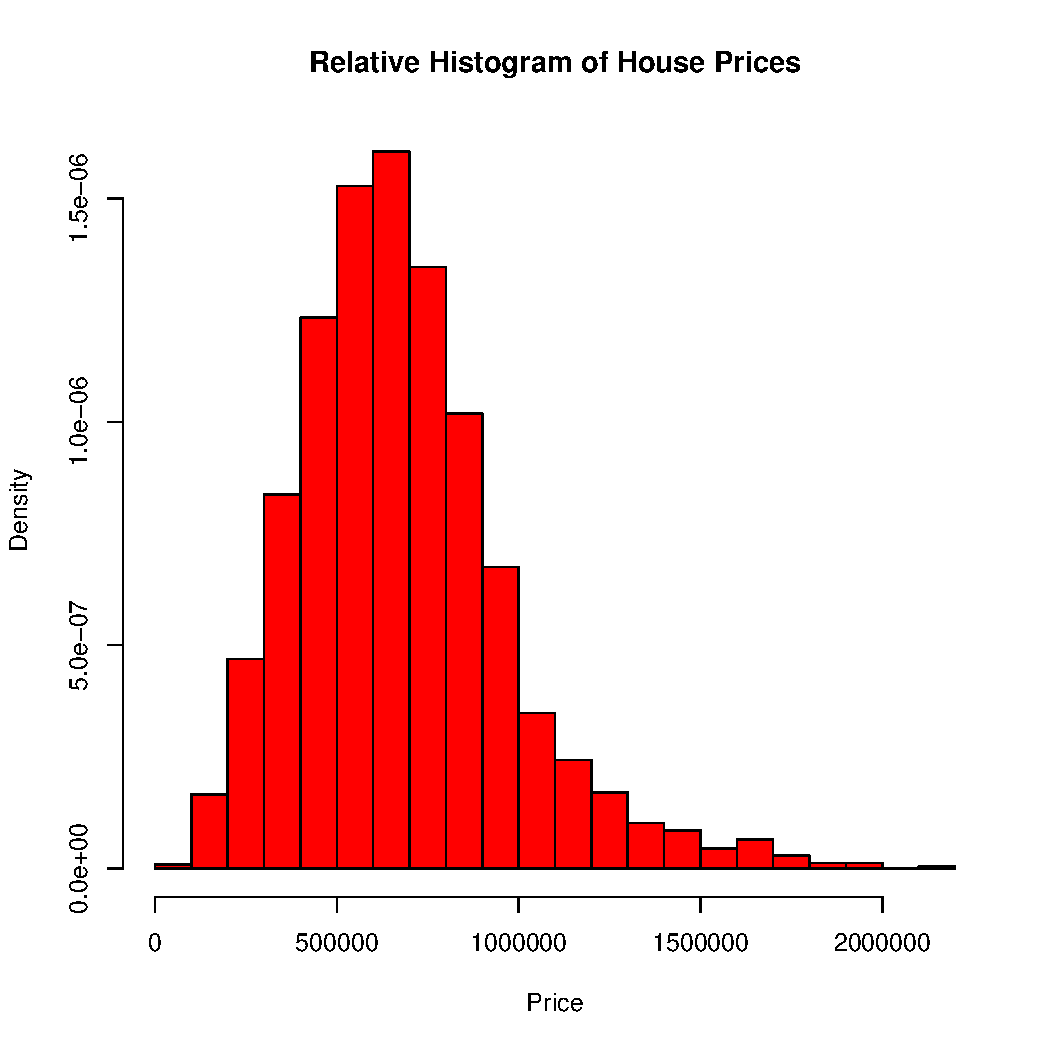
\includegraphics[scale = 0.5, keepaspectratio=true]{../Figures/hist_price}
  \caption{Histogram of House Prices} \label{fig:hist_price}
\end{figure}



\pagebreak
As a comparison, Figure \ref{fig:hist_log_price} shows the histogram of the natural logarithm of
price.

\begin{figure}[h!]
  \centering
  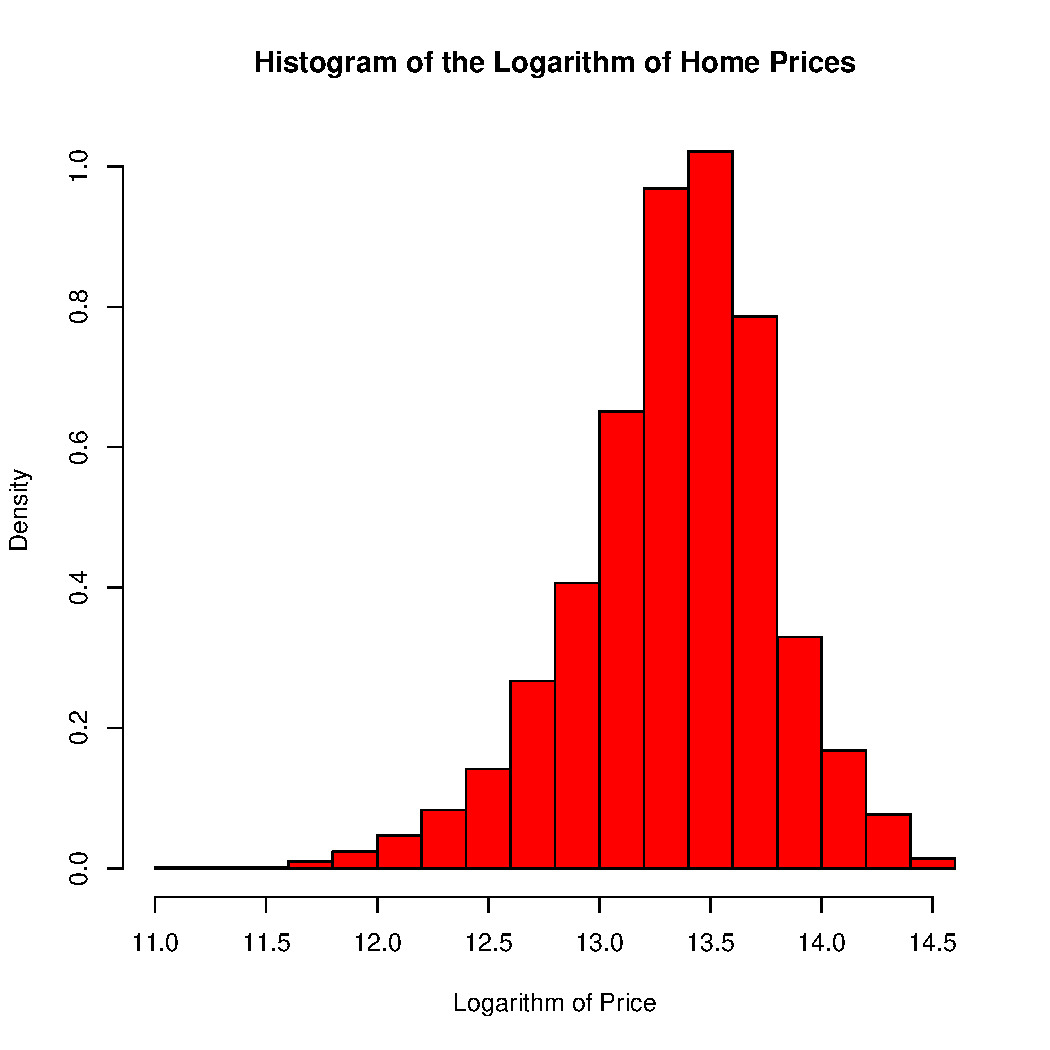
\includegraphics[scale = 0.5, keepaspectratio=true]{../Figures/hist_log_price}
  \caption{Histogram of the Logarithm of Tractor Prices} \label{fig:hist_log_price}
\end{figure}




%%%%%%%%%%%%%%%%%%%%%%%%%%%%%%%%%%%%%%%%
% Linear Regression Models
%%%%%%%%%%%%%%%%%%%%%%%%%%%%%%%%%%%%%%%%


\pagebreak
\subsection{Linear Regression Models of House Prices}


Here I build a regression model with all the variables and price and also another model with the natural logarithm prices.


\begin{table}
\begin{center}
\begin{tabular}{l c c}
\hline
 & Model 1 & Model 2 \\
\hline
(Intercept)       & $-13493752.25309^{***}$ & $-9.86780^{***}$ \\
                  & $(601281.58476)$        & $(0.84272)$      \\
YearBuilt         & $6615.49321^{***}$      & $0.01084^{***}$  \\
                  & $(298.74438)$           & $(0.00042)$      \\
NumBeds           & $92548.13460^{***}$     & $0.13122^{***}$  \\
                  & $(8006.80651)$          & $(0.01122)$      \\
NumBaths          & $26490.99054^{**}$      & $0.07083^{***}$  \\
                  & $(8377.76428)$          & $(0.01174)$      \\
FloorSpace        & $38.40785$              & $0.00002$        \\
                  & $(30.86097)$            & $(0.00004)$      \\
LotSize           & $21.54593^{***}$        & $0.00003^{***}$  \\
                  & $(2.90062)$             & $(0.00000)$      \\
HasGarage         & $130010.15275^{***}$    & $0.28206^{***}$  \\
                  & $(18873.47333)$         & $(0.02645)$      \\
HasEnclPatio      & $27910.39331^{***}$     & $0.05541^{***}$  \\
                  & $(8461.30634)$          & $(0.01186)$      \\
HasSecGate        & $155859.26108^{***}$    & $0.18598^{***}$  \\
                  & $(12498.19417)$         & $(0.01752)$      \\
HasPool           & $72977.97398^{***}$     & $0.07524^{**}$   \\
                  & $(17000.27998)$         & $(0.02383)$      \\
TransitScore      & $36115.28316^{***}$     & $0.06513^{***}$  \\
                  & $(1525.51010)$          & $(0.00214)$      \\
SchoolScore       & $954.30361$             & $0.00913^{***}$  \\
                  & $(1883.35880)$          & $(0.00264)$      \\
TypeOfBuyerRental & $80428.21155^{***}$     & $0.10219^{***}$  \\
                  & $(11282.76745)$         & $(0.01581)$      \\
\hline
R$^2$             & $0.59589$               & $0.67214$        \\
Adj. R$^2$        & $0.59392$               & $0.67055$        \\
Num. obs.         & $2473$                  & $2473$           \\
\hline
\multicolumn{3}{l}{\scriptsize{$^{***}p<0.001$; $^{**}p<0.01$; $^{*}p<0.05$}}
\end{tabular}
\caption{Linear and Logarithmic Models of House Prices}
\label{tab:reg_price_w_log}
\end{center}
\end{table}


The results of Model 1 and Model 2 in Table \ref{tab:reg_price_w_log}
shows the effect of the variables on the dollar price of the
home prices and natural logarithm of . 

From the R squared value, natural log model (Model 2) is a better model to use.


%%%%%%%%%%%%%%%%%%%%%%%%%%%%%%%%%%%%%%%%
\clearpage
\section{Model Specification}
%%%%%%%%%%%%%%%%%%%%%%%%%%%%%%%%%%%%%%%%

\subsection{Variable Reduction}

Next, I can refine the model by removing some explanatory variables that do not have string predictive value. 
The first candidates are those with coefficients that are not statistically significant. 
The results in Table \ref{tab:reg_reduction} are conducted using the natural logarithm prices as we concluded from the previous analysis.


\begin{table}
\begin{center}
\begin{tabular}{l c c c c c}
\hline
 & Model 1 & Model 2 & Model 3 & Model 4 & Model 5 \\
\hline
(Intercept)       & $-9.8678^{***}$ & $-9.8544^{***}$ & $-9.8423^{***}$ & $-9.8162^{***}$ & $-9.7645^{***}$ \\
                  & $(0.8427)$      & $(0.8420)$      & $(0.8438)$      & $(0.8477)$      & $(0.8489)$      \\
TypeOfBuyerRental & $0.1022^{***}$  & $0.1022^{***}$  & $0.1000^{***}$  & $0.0926^{***}$  & $0.0886^{***}$  \\
                  & $(0.0158)$      & $(0.0158)$      & $(0.0158)$      & $(0.0158)$      & $(0.0158)$      \\
YearBuilt         & $0.0108^{***}$  & $0.0108^{***}$  & $0.0108^{***}$  & $0.0108^{***}$  & $0.0108^{***}$  \\
                  & $(0.0004)$      & $(0.0004)$      & $(0.0004)$      & $(0.0004)$      & $(0.0004)$      \\
NumBeds           & $0.1312^{***}$  & $0.1344^{***}$  & $0.1386^{***}$  & $0.1473^{***}$  & $0.1498^{***}$  \\
                  & $(0.0112)$      & $(0.0085)$      & $(0.0084)$      & $(0.0082)$      & $(0.0082)$      \\
NumBaths          & $0.0708^{***}$  & $0.0722^{***}$  & $0.0749^{***}$  & $0.0783^{***}$  & $0.0774^{***}$  \\
                  & $(0.0117)$      & $(0.0113)$      & $(0.0113)$      & $(0.0114)$      & $(0.0114)$      \\
FloorSpace        & $0.0000$        &                 &                 &                 &                 \\
                  & $(0.0000)$      &                 &                 &                 &                 \\
LotSize           & $0.0000^{***}$  & $0.0000^{***}$  & $0.0000^{***}$  & $0.0000^{***}$  & $0.0000^{***}$  \\
                  & $(0.0000)$      & $(0.0000)$      & $(0.0000)$      & $(0.0000)$      & $(0.0000)$      \\
HasGarage         & $0.2821^{***}$  & $0.2902^{***}$  & $0.2953^{***}$  & $0.3015^{***}$  & $0.2978^{***}$  \\
                  & $(0.0265)$      & $(0.0185)$      & $(0.0184)$      & $(0.0185)$      & $(0.0185)$      \\
HasEnclPatio      & $0.0554^{***}$  & $0.0553^{***}$  & $0.0579^{***}$  &                 &                 \\
                  & $(0.0119)$      & $(0.0119)$      & $(0.0119)$      &                 &                 \\
HasSecGate        & $0.1860^{***}$  & $0.1864^{***}$  & $0.1927^{***}$  & $0.1880^{***}$  & $0.1855^{***}$  \\
                  & $(0.0175)$      & $(0.0175)$      & $(0.0174)$      & $(0.0175)$      & $(0.0175)$      \\
HasPool           & $0.0752^{**}$   & $0.0752^{**}$   & $0.0739^{**}$   & $0.0725^{**}$   &                 \\
                  & $(0.0238)$      & $(0.0238)$      & $(0.0239)$      & $(0.0240)$      &                 \\
TransitScore      & $0.0651^{***}$  & $0.0651^{***}$  & $0.0641^{***}$  & $0.0652^{***}$  & $0.0653^{***}$  \\
                  & $(0.0021)$      & $(0.0021)$      & $(0.0021)$      & $(0.0021)$      & $(0.0021)$      \\
SchoolScore       & $0.0091^{***}$  & $0.0090^{***}$  &                 &                 &                 \\
                  & $(0.0026)$      & $(0.0026)$      &                 &                 &                 \\
\hline
R$^2$             & $0.6721$        & $0.6721$        & $0.6705$        & $0.6674$        & $0.6661$        \\
Adj. R$^2$        & $0.6705$        & $0.6707$        & $0.6692$        & $0.6661$        & $0.6650$        \\
Num. obs.         & $2473$          & $2473$          & $2473$          & $2473$          & $2473$          \\
\hline
\multicolumn{6}{l}{\scriptsize{$^{***}p<0.001$; $^{**}p<0.01$; $^{*}p<0.05$}}
\end{tabular}
\caption{Models for the Log. of House Sales}
\label{tab:reg_reduction}
\end{center}
\end{table}


The first column of Table \ref{tab:reg_reduction}
shows the results from the original model of
the logarithm of tractor prices in Table \ref{tab:reg_price_w_log}. 
Model 2 was created with removing the variable FloorSpace due to the insignificance.
Model 3 then also removed SchoolScore. The R squared changed only by minimal amount.
Model 4 I removed whether it has an enclosed patio and then Model 5 removed whether the home has a pool.
Model 5 or the fully reduced model would be the best model due to the R squared not being reduced too much and all variables are significant predictors.

\clearpage
\pagebreak
\subsection{Analysis of Models of Owner-Occupied and Rentals}
The results in Table \ref{tab:reg_buyer} are shown with Models 1-3 showing reductions of insignificant variables with owner occupied properties starting with all variables included in Model 1. Models 4-6 show the reduction of insignificant variables with rental properties starting with all variables included in Model 4. Again, variables were dropped if they were close to the p value of 0.05.
Models 3 and 6 show the best model of Owner Occupied and Rental Houses, respectively. In those models, all variables are statistically significant and R sqaured are minimally affected.


\begin{table}
\begin{center}
\begin{footnotesize}
\begin{tabular}{l c c c c c c}
\hline
 & Model 1 & Model 2 & Model 3 & Model 4 & Model 5 & Model 6 \\
\hline
(Intercept)  & $-10.90967^{***}$ & $-10.86457^{***}$ & $-10.99011^{***}$ & $-8.22131^{***}$ & $-7.91962^{***}$ & $-7.76768^{***}$ \\
             & $(1.04843)$       & $(1.04898)$       & $(1.05460)$       & $(1.39213)$      & $(1.39429)$      & $(1.39351)$      \\
YearBuilt    & $0.01143^{***}$   & $0.01142^{***}$   & $0.01148^{***}$   & $0.00990^{***}$  & $0.00982^{***}$  & $0.00973^{***}$  \\
             & $(0.00052)$       & $(0.00052)$       & $(0.00052)$       & $(0.00069)$      & $(0.00069)$      & $(0.00069)$      \\
NumBeds      & $0.12324^{***}$   & $0.12175^{***}$   & $0.12946^{***}$   & $0.14623^{***}$  & $0.17404^{***}$  & $0.18725^{***}$  \\
             & $(0.01260)$       & $(0.00928)$       & $(0.00916)$       & $(0.02578)$      & $(0.02196)$      & $(0.02119)$      \\
NumBaths     & $0.05065^{***}$   & $0.05180^{***}$   & $0.05643^{***}$   & $0.10865^{***}$  & $0.12531^{***}$  & $0.12449^{***}$  \\
             & $(0.01303)$       & $(0.01258)$       & $(0.01260)$       & $(0.02522)$      & $(0.02433)$      & $(0.02439)$      \\
FloorSpace   & $-0.00002$        &                   &                   & $0.00018$        &                  &                  \\
             & $(0.00005)$       &                   &                   & $(0.00009)$      &                  &                  \\
LotSize      & $0.00003^{***}$   & $0.00003^{***}$   & $0.00003^{***}$   & $0.00004^{***}$  & $0.00005^{***}$  & $0.00004^{***}$  \\
             & $(0.00000)$       & $(0.00000)$       & $(0.00000)$       & $(0.00001)$      & $(0.00001)$      & $(0.00001)$      \\
HasGarage    & $0.33981^{***}$   & $0.33315^{***}$   & $0.33550^{***}$   & $0.09586$        & $0.17029^{***}$  & $0.17901^{***}$  \\
             & $(0.03239)$       & $(0.02415)$       & $(0.02428)$       & $(0.05167)$      & $(0.03280)$      & $(0.03266)$      \\
HasEnclPatio & $0.05639^{***}$   & $0.05970^{***}$   &                   & $0.05186^{*}$    & $0.05373^{*}$    &                  \\
             & $(0.01363)$       & $(0.01361)$       &                   & $(0.02282)$      & $(0.02293)$      &                  \\
HasSecGate   & $0.20097^{***}$   & $0.20759^{***}$   & $0.20305^{***}$   & $0.25584^{**}$   &                  &                  \\
             & $(0.01734)$       & $(0.01719)$       & $(0.01726)$       & $(0.09819)$      &                  &                  \\
HasPool      & $0.09698^{***}$   & $0.09616^{***}$   & $0.09439^{***}$   & $-0.04440$       & $-0.04657$       &                  \\
             & $(0.02455)$       & $(0.02460)$       & $(0.02474)$       & $(0.06656)$      & $(0.06687)$      &                  \\
TransitScore & $0.05559^{***}$   & $0.05377^{***}$   & $0.05488^{***}$   & $0.07474^{***}$  & $0.07511^{***}$  & $0.07536^{***}$  \\
             & $(0.00272)$       & $(0.00265)$       & $(0.00266)$       & $(0.00429)$      & $(0.00429)$      & $(0.00430)$      \\
SchoolScore  & $0.00914^{**}$    &                   &                   & $0.00329$        &                  &                  \\
             & $(0.00319)$       &                   &                   & $(0.00476)$      &                  &                  \\
\hline
R$^2$        & $0.56433$         & $0.56195$         & $0.55662$         & $0.68415$        & $0.67972$        & $0.67753$        \\
Adj. R$^2$   & $0.56130$         & $0.55946$         & $0.55439$         & $0.68014$        & $0.67677$        & $0.67531$        \\
Num. obs.    & $1594$            & $1594$            & $1594$            & $879$            & $879$            & $879$            \\
\hline
\multicolumn{7}{l}{\tiny{$^{***}p<0.001$; $^{**}p<0.01$; $^{*}p<0.05$}}
\end{tabular}
\end{footnotesize}
\caption{Separate Models by Type of Buyer}
\label{tab:reg_buyer}
\end{center}
\end{table}

\pagebreak
\clearpage
\subsection{Compare Models of Owner-Occupied and Rentals}


We can also test for all of the differences at the same time
by using an $F$-test.  
% 
The $F$-statistic has a value of 

$$ 
7.91
$$

This is a high value for the $F$-statistic. 
We reject the null that all 
coefficients are equal across both samples .




%%%%%%%%%%%%%%%%%%%%%%%%%%%%%%%%%%%%%%%%
%\end{document}
%%%%%%%%%%%%%%%%%%%%%%%%%%%%%%%%%%%%%%%%


\pagebreak
\chapter{Transforming the Explanatory Variables}
%\documentclass[11pt]{paper}
%\usepackage{fullpage}
%\usepackage{palatino}
%\usepackage{amsfonts,amsmath,amssymb}
%% \usepackage{graphicx}
%
%\usepackage{listings}
%\usepackage{textcomp}
%\usepackage{color}
%
%\definecolor{dkgreen}{rgb}{0,0.6,0}
%\definecolor{gray}{rgb}{0.5,0.5,0.5}
%\definecolor{mauve}{rgb}{0.58,0,0.82}
%
%\lstset{frame=tb,
%  language=R,
%  aboveskip=3mm,
%  belowskip=3mm,
%  showstringspaces=false,
%  columns=flexible,
%  basicstyle={\small\ttfamily},
%  numbers=none,
%  numberstyle=\tiny\color{gray},
%  keywordstyle=\color{blue},
%  commentstyle=\color{dkgreen},
%  stringstyle=\color{mauve},
%  breaklines=true,
%  breakatwhitespace=true,
%  tabsize=3
%}
%
%
%
%\ifx\pdftexversion\undefined
%    \usepackage[dvips]{graphicx}
%\else
%    \usepackage[pdftex]{graphicx}
%    \usepackage{epstopdf}
%    \epstopdfsetup{suffix=}
%\fi
%
%\usepackage{subfig}
%
%
%% This allows pdflatex to print the curly quotes in the
%% significance codes in the output of the GAM.
%\UseRawInputEncoding
%
%\begin{document}
%
%%%%%%%%%%%%%%%%%%%%%%%%%%%%%%%%%%%%%%%%%
%% Problem Set 7
%%%%%%%%%%%%%%%%%%%%%%%%%%%%%%%%%%%%%%%%%
%
%\pagestyle{empty}
%{\noindent\bf Spring 2023 \hfill Brandon~Parmanand}
%\vskip 16pt
%\centerline{\bf University of Central Florida}
%\centerline{\bf College of Business}
%\vskip 16pt
%\centerline{\bf QMB 6911}
%\centerline{\bf Capstone Project in Business Analytics}
%\vskip 10pt
%\centerline{\bf Solutions:  Problem Set \#7}
%\vskip 32pt
%\noindent
%% 
%\section{Data Description}
%
%This analysis follows the script \texttt{PS7.R} to produce a more accurate model for used tractor prices with the data from \texttt{homesales.dat} in the \texttt{Data} folder. 

I will revisit the recommended linear model.
I will further investigate nonlinear relationships
by incorporating another nonlinear but parametric specification
for variables.
This parametric analysis will be performed
using the Box-Tidwell framework
to investigate whether the value of these characteristics
are best described with parametric nonlinear forms. 

%%%%%%%%%%%%%%%%%%%%%%%%%%%%%%%%%%%%%%%%
\section{Linear Regression Model}
%%%%%%%%%%%%%%%%%%%%%%%%%%%%%%%%%%%%%%%%

\subsection{Suggested Linear Regression Model}
A natural staring point is the recommended linear model
from previous which we can see in Table \ref{tab:reg_comp}. 

% 

\begin{table}
\begin{center}
\begin{tabular}{l c}
\hline
 & Model 1 \\
\hline
(Intercept)       & $12.2109^{***}$ \\
                  & $(0.0333)$      \\
TypeOfBuyerRental & $0.1126^{***}$  \\
                  & $(0.0160)$      \\
Age               & $-0.0108^{***}$ \\
                  & $(0.0004)$      \\
NumBeds2          & $0.2209^{***}$  \\
                  & $(0.0260)$      \\
NumBeds3          & $0.4205^{***}$  \\
                  & $(0.0314)$      \\
NumBeds4          & $0.6106^{***}$  \\
                  & $(0.0346)$      \\
NumBeds6          & $0.7039^{***}$  \\
                  & $(0.0562)$      \\
NumBeds8          & $1.0794^{***}$  \\
                  & $(0.0612)$      \\
NumBaths2         & $0.0721^{***}$  \\
                  & $(0.0139)$      \\
NumBaths3         & $0.1033^{***}$  \\
                  & $(0.0271)$      \\
LotSize           & $0.0000^{***}$  \\
                  & $(0.0000)$      \\
HasGarage         & $0.2638^{***}$  \\
                  & $(0.0194)$      \\
HasSecGate        & $0.2238^{***}$  \\
                  & $(0.0180)$      \\
TransitScore      & $0.0636^{***}$  \\
                  & $(0.0030)$      \\
\hline
R$^2$             & $0.6745$        \\
Adj. R$^2$        & $0.6728$        \\
Num. obs.         & $2473$          \\
\hline
\multicolumn{2}{l}{\scriptsize{$^{***}p<0.001$; $^{**}p<0.01$; $^{*}p<0.05$}}
\end{tabular}
\caption{Models for the Log. of House Sales}
\label{tab:reg_comp}
\end{center}
\end{table}

% 
There are houses that were built in 2021 so in order to account for this in the model, an edit was made to calculate age by taking 2022- Year Built. Additionally, Number of Beds and Numbers of Bathrooms were treated as factors in the model as they more so categorize the houses.
%
\clearpage


%%%%%%%%%%%%%%%%%%%%%%%%%%%%%%%%%%%%%%%%
% \clearpage
\section{Nonlinear Specifications}
%%%%%%%%%%%%%%%%%%%%%%%%%%%%%%%%%%%%%%%%

%\pagebreak
\subsection{The Box--Tidwell Transformation}

The Box--Tidwell function tests for non-linear relationships
to the mean of the dependent variable.
The nonlinearity is in the form of an
exponential transformation in the form of the Box-Cox
transformation, except that the transformation is taken
on the explanatory variables.


\subsubsection{Transformation of Lot Size}


Performing the transformation on the Lot Size variable
produces a modified form of the linear model. The exponentis significantly differnt from 0. WItrh a small positive value that suggest an increasing relationship then leveling off to a slower increase. 

\begin{verbatim} MLE of lambda Score Statistic (z)  Pr(>|z|)    
       -0.2736             -3.6889 0.0002252 ***
---
Signif. codes:  0 �***� 0.001 �**� 0.01 �*� 0.05 �.� 0.1 � � 1

iterations =  3 
\end{verbatim}



\subsubsection{Transformation of Age}


\begin{verbatim} MLE of lambda Score Statistic (z)  Pr(>|z|)    
       0.49715              6.4677 9.949e-11 ***
---
Signif. codes:  0 �***� 0.001 �**� 0.01 �*� 0.05 �.� 0.1 � � 1

iterations =  3 
\end{verbatim}

This coefficient is significantly different than 0. With a positive value that suggest not quite a linear relationship but it is an increasing relationship with it leveling off and increasing at a slower rate.  

\subsubsection{Transformation of Transit Score}


\begin{verbatim} MLE of lambda Score Statistic (z) Pr(>|z|)
        1.1833              1.0571   0.2905

iterations =  3 
\end{verbatim}

The transit score coefficient is not statistically significant but it is close to 1 showing close to linear realationship.

Since a nonlinear relationship was detected with age and lot size,
I will next estimate a model
with nonlinearity in all three continuous variables.


\subsubsection{Transformation of All Three Continuous Variables}


\begin{verbatim}             MLE of lambda Score Statistic (z)  Pr(>|z|)    
TransitScore       1.20854              1.2318 0.2180097    
Age                0.50460              6.4167 1.392e-10 ***
LotSize           -0.27686             -3.6641 0.0002482 ***
---
Signif. codes:  0 �***� 0.001 �**� 0.01 �*� 0.05 �.� 0.1 � � 1

iterations =  3 
\end{verbatim}


The performance is similar to the other models with
forms of nonlinearity .



\pagebreak
\section{Linear Approximation of the Box--Tidwell Transformation}

I created three variables 
\texttt{bt\_trans\_log\_trans}, \texttt{bt\_age\_log\_age}, and \texttt{bt\_lot\_log\_lot}, 
all of which were created by a transformation of the form $f(x) = x\cdot\log(x)$. 
Table \ref{tab:reg_bt_lin} collects the results
of the set of models from the nonlinear approximation to the models with the three forms of nonlinearity.
Model 1 is the linear regression model with  
the approximation of the transformation applied to transit score. 
Models 2 and 3
have the same specification as the other one, 
except that the transit score variable is replaced with
the variables for age and lot size, respectively. 
The coefficient on \texttt{bt\_age\_log\_age}
is the most statistically significant. 
And the coefficient on \texttt{bt\_lot\_log\_lot} is also statistically signifcant. 
This implies, just as the Box-Tidwell statistic predicts, 
a nonlinear relationship exists for the value of age and lot size.
The transit score is not statistically significant as the other two
indicating that a linear relationship suffices for the decline in value from transit score.


\begin{table}
\begin{center}
\begin{tabular}{l c c c}
\hline
 & Model 1 & Model 2 & Model 3 \\
\hline
(Intercept)           & $12.25507^{***}$ & $12.27956^{***}$ & $11.89089^{***}$ \\
                      & $(0.05344)$      & $(0.03468)$      & $(0.09288)$      \\
TypeOfBuyerRental     & $0.10997^{***}$  & $0.11437^{***}$  & $0.11362^{***}$  \\
                      & $(0.01621)$      & $(0.01590)$      & $(0.01599)$      \\
Age                   & $-0.01083^{***}$ & $-0.03428^{***}$ & $-0.01089^{***}$ \\
                      & $(0.00042)$      & $(0.00365)$      & $(0.00042)$      \\
NumBeds2              & $0.22205^{***}$  & $0.22090^{***}$  & $0.20754^{***}$  \\
                      & $(0.02600)$      & $(0.02576)$      & $(0.02616)$      \\
NumBeds3              & $0.41967^{***}$  & $0.41973^{***}$  & $0.40137^{***}$  \\
                      & $(0.03141)$      & $(0.03114)$      & $(0.03174)$      \\
NumBeds4              & $0.59709^{***}$  & $0.60678^{***}$  & $0.59744^{***}$  \\
                      & $(0.03693)$      & $(0.03437)$      & $(0.03474)$      \\
NumBeds6              & $0.68745^{***}$  & $0.69817^{***}$  & $0.72136^{***}$  \\
                      & $(0.05831)$      & $(0.05573)$      & $(0.05624)$      \\
NumBeds8              & $1.06090^{***}$  & $1.07728^{***}$  & $1.11651^{***}$  \\
                      & $(0.06363)$      & $(0.06068)$      & $(0.06185)$      \\
NumBaths2             & $0.07221^{***}$  & $0.07219^{***}$  & $0.07012^{***}$  \\
                      & $(0.01387)$      & $(0.01376)$      & $(0.01384)$      \\
NumBaths3             & $0.10338^{***}$  & $0.10791^{***}$  & $0.10408^{***}$  \\
                      & $(0.02715)$      & $(0.02694)$      & $(0.02708)$      \\
LotSize               & $0.00004^{***}$  & $0.00004^{***}$  & $0.00053^{***}$  \\
                      & $(0.00000)$      & $(0.00000)$      & $(0.00014)$      \\
HasGarage             & $0.26282^{***}$  & $0.26785^{***}$  & $0.24900^{***}$  \\
                      & $(0.01941)$      & $(0.01924)$      & $(0.01975)$      \\
HasSecGate            & $0.22309^{***}$  & $0.22254^{***}$  & $0.22569^{***}$  \\
                      & $(0.01804)$      & $(0.01788)$      & $(0.01798)$      \\
TransitScore          & $0.03918$        & $0.06332^{***}$  & $0.06433^{***}$  \\
                      & $(0.02329)$      & $(0.00296)$      & $(0.00298)$      \\
bt\_trans\_log\_trans & $0.00923$        &                  &                  \\
                      & $(0.00874)$      &                  &                  \\
bt\_age\_log\_age     &                  & $0.00608^{***}$  &                  \\
                      &                  & $(0.00094)$      &                  \\
bt\_lot\_log\_lot     &                  &                  & $-0.00005^{***}$ \\
                      &                  &                  & $(0.00001)$      \\
\hline
R$^2$                 & $0.67469$        & $0.67999$        & $0.67634$        \\
Adj. R$^2$            & $0.67284$        & $0.67817$        & $0.67449$        \\
Num. obs.             & $2473$           & $2473$           & $2473$           \\
\hline
\multicolumn{4}{l}{\scriptsize{$^{***}p<0.001$; $^{**}p<0.01$; $^{*}p<0.05$}}
\end{tabular}
\caption{Linear Approximation of Box-Tidwell Transformations for House Prices}
\label{tab:reg_bt_lin}
\end{center}
\end{table}



\pagebreak
\section{Comparison of Candidate Models}

Comparing the three models, Age and Lot Size were both significantly signifcant with p less than $0.001$ but the model with the age transformation had the highest R squared. I created a variable \texttt{age\_bt}
by raising age to the optimal exponent 
$\hat{\lambda} = 0.49715$. 
Then, I included this variable in the place of 
the age variables a the linear regression model.
% 
Table \ref{tab:reg_sq_horse_bt} collects the results
of the set of models from the two forms of nonlinearity.
Model 1 is the approximation to the Box-Tidwell transformation
from Model 2 of Table \ref{tab:reg_bt_lin}. 
Model 2
has the same specification as the approximate transformation, 
except that the age variable is transformed using the optimal
exponent for the Box-Tidwell transformation. 
% 
The last model has the highest R-squared
among the ones we have estimated, 
with only a slight improvement over the linear approximation.
Again, the differences are marginal, so the practical recommendation
is model with the $f(x) = x\cdot\log(x)$.



\begin{table}
\begin{center}
\begin{tabular}{l c c}
\hline
 & Model 1 & Model 2 \\
\hline
(Intercept)       & $12.27956^{***}$ & $12.34070^{***}$ \\
                  & $(0.03468)$      & $(0.03395)$      \\
TypeOfBuyerRental & $0.11437^{***}$  & $0.11404^{***}$  \\
                  & $(0.01590)$      & $(0.01589)$      \\
Age               & $-0.03428^{***}$ &                  \\
                  & $(0.00365)$      &                  \\
NumBeds2          & $0.22090^{***}$  & $0.22147^{***}$  \\
                  & $(0.02576)$      & $(0.02575)$      \\
NumBeds3          & $0.41973^{***}$  & $0.42032^{***}$  \\
                  & $(0.03114)$      & $(0.03113)$      \\
NumBeds4          & $0.60678^{***}$  & $0.60720^{***}$  \\
                  & $(0.03437)$      & $(0.03435)$      \\
NumBeds6          & $0.69817^{***}$  & $0.69834^{***}$  \\
                  & $(0.05573)$      & $(0.05571)$      \\
NumBeds8          & $1.07728^{***}$  & $1.07896^{***}$  \\
                  & $(0.06068)$      & $(0.06066)$      \\
NumBaths2         & $0.07219^{***}$  & $0.07189^{***}$  \\
                  & $(0.01376)$      & $(0.01375)$      \\
NumBaths3         & $0.10791^{***}$  & $0.10731^{***}$  \\
                  & $(0.02694)$      & $(0.02692)$      \\
LotSize           & $0.00004^{***}$  & $0.00004^{***}$  \\
                  & $(0.00000)$      & $(0.00000)$      \\
HasGarage         & $0.26785^{***}$  & $0.26760^{***}$  \\
                  & $(0.01924)$      & $(0.01923)$      \\
HasSecGate        & $0.22254^{***}$  & $0.22260^{***}$  \\
                  & $(0.01788)$      & $(0.01787)$      \\
TransitScore      & $0.06332^{***}$  & $0.06332^{***}$  \\
                  & $(0.00296)$      & $(0.00296)$      \\
bt\_age\_log\_age & $0.00608^{***}$  &                  \\
                  & $(0.00094)$      &                  \\
age\_bt           &                  & $-0.08524^{***}$ \\
                  &                  & $(0.00316)$      \\
\hline
R$^2$             & $0.67999$        & $0.68005$        \\
Adj. R$^2$        & $0.67817$        & $0.67836$        \\
Num. obs.         & $2473$           & $2473$           \\
\hline
\multicolumn{3}{l}{\scriptsize{$^{***}p<0.001$; $^{**}p<0.01$; $^{*}p<0.05$}}
\end{tabular}
\caption{Alternate Models for House Prices}
\label{tab:reg_sq_horse_bt}
\end{center}
\end{table}




%%%%%%%%%%%%%%%%%%%%%%%%%%%%%%%%%%%%%%%%
%\end{document}
%%%%%%%%%%%%%%%%%%%%%%%%%%%%%%%%%%%%%%%%


\pagebreak
\chapter{Nonparametric Regression Models}
%\documentclass[11pt]{paper}
%\usepackage{palatino}
%\usepackage{amsfonts,amsmath,amssymb}
%% \usepackage{graphicx}
%
%\usepackage{listings}
%\usepackage{textcomp}
%\usepackage{color}
%
%\definecolor{dkgreen}{rgb}{0,0.6,0}
%\definecolor{gray}{rgb}{0.5,0.5,0.5}
%\definecolor{mauve}{rgb}{0.58,0,0.82}
%
%\lstset{frame=tb,
%  language=R,
%  aboveskip=3mm,
%  belowskip=3mm,
%  showstringspaces=false,
%  columns=flexible,
%  basicstyle={\small\ttfamily},
%  numbers=none,
%  numberstyle=\tiny\color{gray},
%  keywordstyle=\color{blue},
%  commentstyle=\color{dkgreen},
%  stringstyle=\color{mauve},
%  breaklines=true,
%  breakatwhitespace=true,
%  tabsize=3
%}
%
%
%
%\ifx\pdftexversion\undefined
%    \usepackage[dvips]{graphicx}
%\else
%    \usepackage[pdftex]{graphicx}
%    \usepackage{epstopdf}
%    \epstopdfsetup{suffix=}
%\fi
%
%\usepackage{subfig}
%
%
%% This allows pdflatex to print the curly quotes in the
%% significance codes in the output of the GAM.
%\UseRawInputEncoding
%
%\begin{document}
%
%%%%%%%%%%%%%%%%%%%%%%%%%%%%%%%%%%%%%%%%%
%% Problem Set 8
%%%%%%%%%%%%%%%%%%%%%%%%%%%%%%%%%%%%%%%%%
%
%\pagestyle{empty}
%{\noindent\bf Spring 2023 \hfill Brandon~Parmanand}
%\vskip 16pt
%\centerline{\bf University of Central Florida}
%\centerline{\bf College of Business}
%\vskip 16pt
%\centerline{\bf QMB 6911}
%\centerline{\bf Capstone Project in Business Analytics}
%\vskip 10pt
%\centerline{\bf Solutions:  Problem Set \#8}
%\vskip 32pt
%\noindent
%% 
%
%
%{\color{red} 
%Quick comments:
%Excellent work; no major problems with modeling decisions.
%Each of you made different decisions with respect to model specification
%and built models of similar accuracy.
%The implementation of FWL regressions and nonparametric/semiparametric models was well done.
%
%The only part that I did not find was a comparison of the GAM vs. the Box-Tidwell modeling framework (please correct me if I am wrong). Other than that minor misstep, this was great.
%}
%
%\section{Data Description}
%
%This analysis follows the script \texttt{PS8.R} to produce a more accurate model for used tractor prices with the data from \texttt{HomeSales.dat} in the \texttt{Data} folder. 
I will revisit the recommended linear model,
which included a Box Tildwell specification for age. 
I will investigate this nonlinear relationship
by incorporating a nonparametric specification
for the value of age. 
Similarly, for the other continuous variables Lot Size and Transit Score, 
to investigate whether these forms of depreciation
are best described with nonlinear forms. 


%%%%%%%%%%%%%%%%%%%%%%%%%%%%%%%%%%%%%%%%
\clearpage
\section{Linear Regression Model}
%%%%%%%%%%%%%%%%%%%%%%%%%%%%%%%%%%%%%%%%

 

\subsection{Box Tildwell Specification for Age}

% 

\begin{table}
\begin{center}
\begin{tabular}{l c}
\hline
 & Model 1 \\
\hline
(Intercept)       & $12.27956^{***}$ \\
                  & $(0.03468)$      \\
TypeOfBuyerRental & $0.11437^{***}$  \\
                  & $(0.01590)$      \\
Age               & $-0.03428^{***}$ \\
                  & $(0.00365)$      \\
NumBeds2          & $0.22090^{***}$  \\
                  & $(0.02576)$      \\
NumBeds3          & $0.41973^{***}$  \\
                  & $(0.03114)$      \\
NumBeds4          & $0.60678^{***}$  \\
                  & $(0.03437)$      \\
NumBeds6          & $0.69817^{***}$  \\
                  & $(0.05573)$      \\
NumBeds8          & $1.07728^{***}$  \\
                  & $(0.06068)$      \\
NumBaths2         & $0.07219^{***}$  \\
                  & $(0.01376)$      \\
NumBaths3         & $0.10791^{***}$  \\
                  & $(0.02694)$      \\
LotSize           & $0.00004^{***}$  \\
                  & $(0.00000)$      \\
HasGarage         & $0.26785^{***}$  \\
                  & $(0.01924)$      \\
HasSecGate        & $0.22254^{***}$  \\
                  & $(0.01788)$      \\
TransitScore      & $0.06332^{***}$  \\
                  & $(0.00296)$      \\
bt\_age\_log\_age & $0.00608^{***}$  \\
                  & $(0.00094)$      \\
\hline
R$^2$             & $0.67999$        \\
Adj. R$^2$        & $0.67817$        \\
Num. obs.         & $2473$           \\
\hline
\multicolumn{2}{l}{\scriptsize{$^{***}p<0.001$; $^{**}p<0.01$; $^{*}p<0.05$}}
\end{tabular}
\caption{Age BT Model for Home Prices}
\label{tab:reg_bt_age}
\end{center}
\end{table}

% 

The results of this regression specification are shown in 
Table \ref{tab:reg_bt_age}. 
The BT Age variable has a coefficient of 
% $6.082e-03$,
$6.082\times10^{-3}$,  
which is larger than the standard error of 
% $9.404e-03$, 
$9.404\times10^{-3}$, 
which is evidence against the null hypothesis of a positive or zero coefficient. 
I conclude that the log of the sale price does decline for older homes. 


%	With the squared horsepower variable, the $\bar{R}^2$ is $0.6503$, indicating that it is a slightly stronger model than the others we considered. 
%	The $F$-statistic is large, indicating that it is a better candidate than the simple average log sale price. 
%	The new BT age variable is statistically significant and the theory behind it is sound, since above a certain point. 
%	This new model is improved over the previous models with other specifications for age.
Next, I will attempt to improve on this specification. 





%%%%%%%%%%%%%%%%%%%%%%%%%%%%%%%%%%%%%%%%
\clearpage
\section{Nonlinear Specifications}
%%%%%%%%%%%%%%%%%%%%%%%%%%%%%%%%%%%%%%%%


% \clearpage
\subsection{Nonparametric Specification for Age}


The specification in 
Table \ref{tab:reg_bt_age}
assumes a Box Tildwell form for
the relationship between price and age. 
To consider the age variable alone, 
while accounting for the effects of other variables, 
one can fit a nonparametric model to the residuals 
from a model of house prices, 
after regressing house prices on the other variables. 
This leaves only the variation in house prices that is not explained by the other variables. 
Going one step further, perform the same transformation to the age variable:
take the residuals from a model of age, 
after regressing age on the other variables. 
This allows a model that would fit exactly the same as if it were estimated within a full model with all variables included. 

The models shown in
Table \ref{tab:reg_bt_age_fwl}
illustrate this possibility. 
Model 1 is the original model in 
Table \ref{tab:reg_bt_age}. 
Model 2 is a regression omitting the age variables. 
Model 3 is a regression to predict age with the other explanatory variables in Model 2.
Model 4 is a regression to predict BT age with the other explanatory variables in Model 2.
Finally, Model 5 shows the coefficients for age
from a regression of the residuals of Model 2
on the residuals from Model 3. 
Notice that these coefficients match those in Model 1. 
You might notice a slight difference in the standard errors, however, 
because these are calculated assuming coefficients 
for two variables, age and BT age,
rather than the full suite of ten parameters.
This equivalence of the coefficients can be used to fit
nonlinear models between a pair of variables by 
partialing out the effect of the other variables.


\begin{table}
\begin{center}
\begin{footnotesize}
\begin{tabular}{l c c c c c}
\hline
 & Original (1) & Reduced (2) & Age (3) & Age. BT. (4) & FWL Age (5) \\
\hline
(Intercept)       & $12.27956^{***}$ & $12.09348^{***}$ & $10.82068^{***}$ & $30.40148^{***}$ &                  \\
                  & $(0.03468)$      & $(0.03722)$      & $(1.59294)$      & $(6.17785)$      &                  \\
TypeOfBuyerRental & $0.11437^{***}$  & $0.05066^{**}$   & $5.70467^{***}$  & $21.68169^{***}$ &                  \\
                  & $(0.01590)$      & $(0.01789)$      & $(0.76573)$      & $(2.96969)$      &                  \\
Age               & $-0.03428^{***}$ &                  &                  &                  &                  \\
                  & $(0.00365)$      &                  &                  &                  &                  \\
NumBeds2          & $0.22090^{***}$  & $0.21786^{***}$  & $0.27924$        & $1.07401$        &                  \\
                  & $(0.02576)$      & $(0.02932)$      & $(1.25470)$      & $(4.86603)$      &                  \\
NumBeds3          & $0.41973^{***}$  & $0.41369^{***}$  & $0.62368$        & $2.52189$        &                  \\
                  & $(0.03114)$      & $(0.03544)$      & $(1.51679)$      & $(5.88251)$      &                  \\
NumBeds4          & $0.60678^{***}$  & $0.61552^{***}$  & $-0.45182$       & $-1.11001$       &                  \\
                  & $(0.03437)$      & $(0.03911)$      & $(1.67365)$      & $(6.49083)$      &                  \\
NumBeds6          & $0.69817^{***}$  & $0.71277^{***}$  & $-0.81578$       & $-2.19939$       &                  \\
                  & $(0.05573)$      & $(0.06342)$      & $(2.71421)$      & $(10.52639)$     &                  \\
NumBeds8          & $1.07728^{***}$  & $1.12632^{***}$  & $-4.32464$       & $-16.31485$      &                  \\
                  & $(0.06068)$      & $(0.06903)$      & $(2.95412)$      & $(11.45684)$     &                  \\
NumBaths2         & $0.07219^{***}$  & $0.07575^{***}$  & $-0.34009$       & $-1.33279$       &                  \\
                  & $(0.01376)$      & $(0.01566)$      & $(0.66996)$      & $(2.59826)$      &                  \\
NumBaths3         & $0.10791^{***}$  & $0.11104^{***}$  & $-0.71642$       & $-3.52346$       &                  \\
                  & $(0.02694)$      & $(0.03064)$      & $(1.31142)$      & $(5.08601)$      &                  \\
LotSize           & $0.00004^{***}$  & $0.00004^{***}$  & $-0.00012$       & $-0.00046$       &                  \\
                  & $(0.00000)$      & $(0.00000)$      & $(0.00018)$      & $(0.00069)$      &                  \\
HasGarage         & $0.26785^{***}$  & $0.21408^{***}$  & $4.58242^{***}$  & $16.98939^{***}$ &                  \\
                  & $(0.01924)$      & $(0.02178)$      & $(0.93185)$      & $(3.61395)$      &                  \\
HasSecGate        & $0.22254^{***}$  & $0.19835^{***}$  & $2.34684^{**}$   & $9.25280^{**}$   &                  \\
                  & $(0.01788)$      & $(0.02032)$      & $(0.86937)$      & $(3.37163)$      &                  \\
TransitScore      & $0.06332^{***}$  & $0.06732^{***}$  & $-0.34281^{*}$   & $-1.27462^{*}$   &                  \\
                  & $(0.00296)$      & $(0.00336)$      & $(0.14398)$      & $(0.55840)$      &                  \\
bt\_age\_log\_age & $0.00608^{***}$  &                  &                  &                  &                  \\
                  & $(0.00094)$      &                  &                  &                  &                  \\
age\_resid        &                  &                  &                  &                  & $-0.03428^{***}$ \\
                  &                  &                  &                  &                  & $(0.00364)$      \\
age\_2\_resid     &                  &                  &                  &                  & $0.00608^{***}$  \\
                  &                  &                  &                  &                  & $(0.00094)$      \\
\hline
R$^2$             & $0.67999$        & $0.58512$        & $0.02593$        & $0.02498$        & $0.22867$        \\
Adj. R$^2$        & $0.67817$        & $0.58310$        & $0.02118$        & $0.02023$        & $0.22804$        \\
Num. obs.         & $2473$           & $2473$           & $2473$           & $2473$           & $2473$           \\
\hline
\multicolumn{6}{l}{\tiny{$^{***}p<0.001$; $^{**}p<0.01$; $^{*}p<0.05$}}
\end{tabular}
\end{footnotesize}
\caption{BT Model for House Prices: FWL Regressions}
\label{tab:reg_bt_age_fwl}
\end{center}
\end{table}


\pagebreak 
To illustrate the fit of the model, 
Figure \ref{fig:dev_vs_age} shows a scatter plot 
of the residual log prices on age. 
The observations are shown in blue
and the fitted values are shown in red.
The variation in the fitted values results from the 
fact that it is not plotted against the transformed excess age variable used in the regressions.


\begin{figure}[h!]
  \centering
  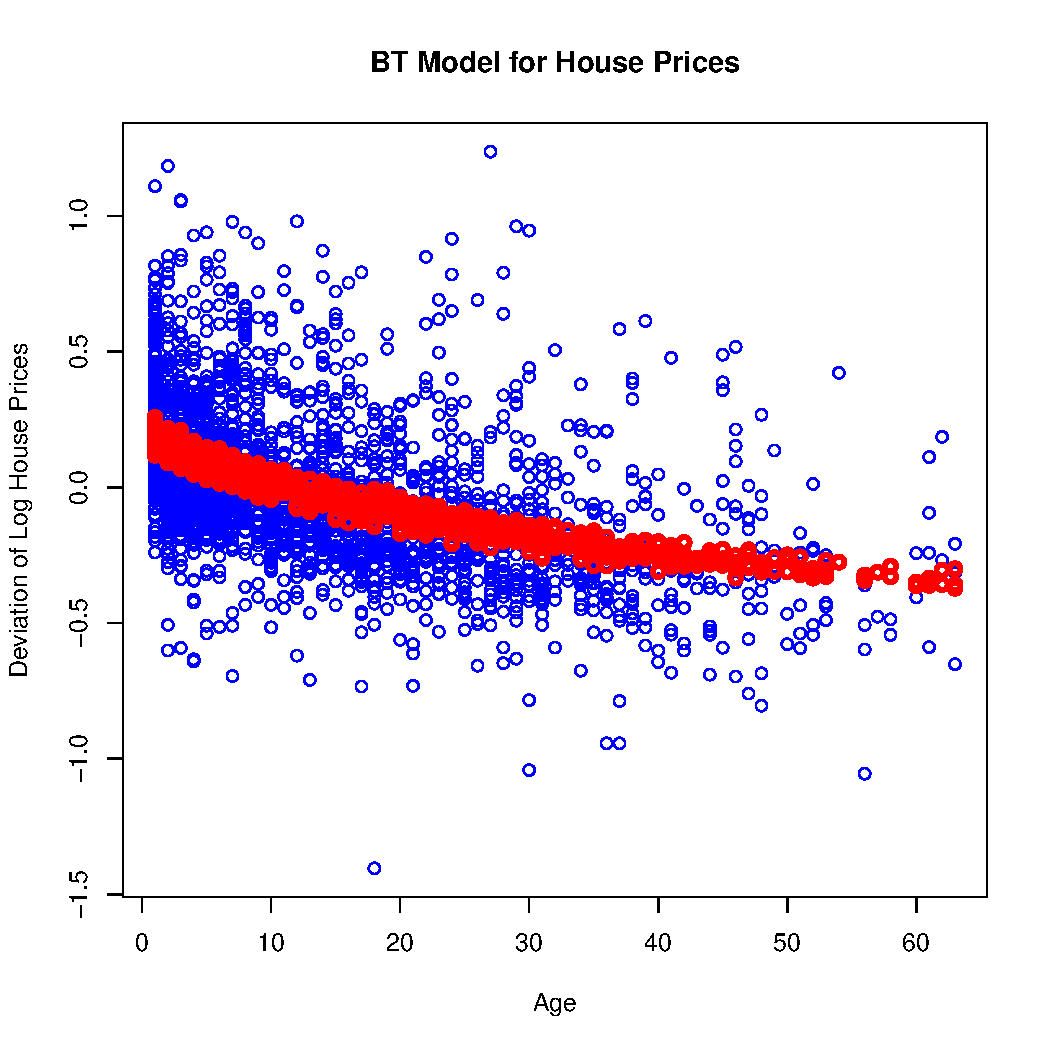
\includegraphics[scale = 0.5, keepaspectratio=true]{../Figures/dev_vs_age}
  \caption{Linear-Box Tildwell Model for House Prices} \label{fig:dev_vs_age}
\end{figure}



\pagebreak
As a comparison, Figure \ref{fig:dev_vs_age_dev} 
augments the above by showing the plot against the 
residuals from the regression for age:
the ``excess age'' compared to what would be 
expected given the other characteristics of a house.


\begin{figure}[h!]
  \centering
  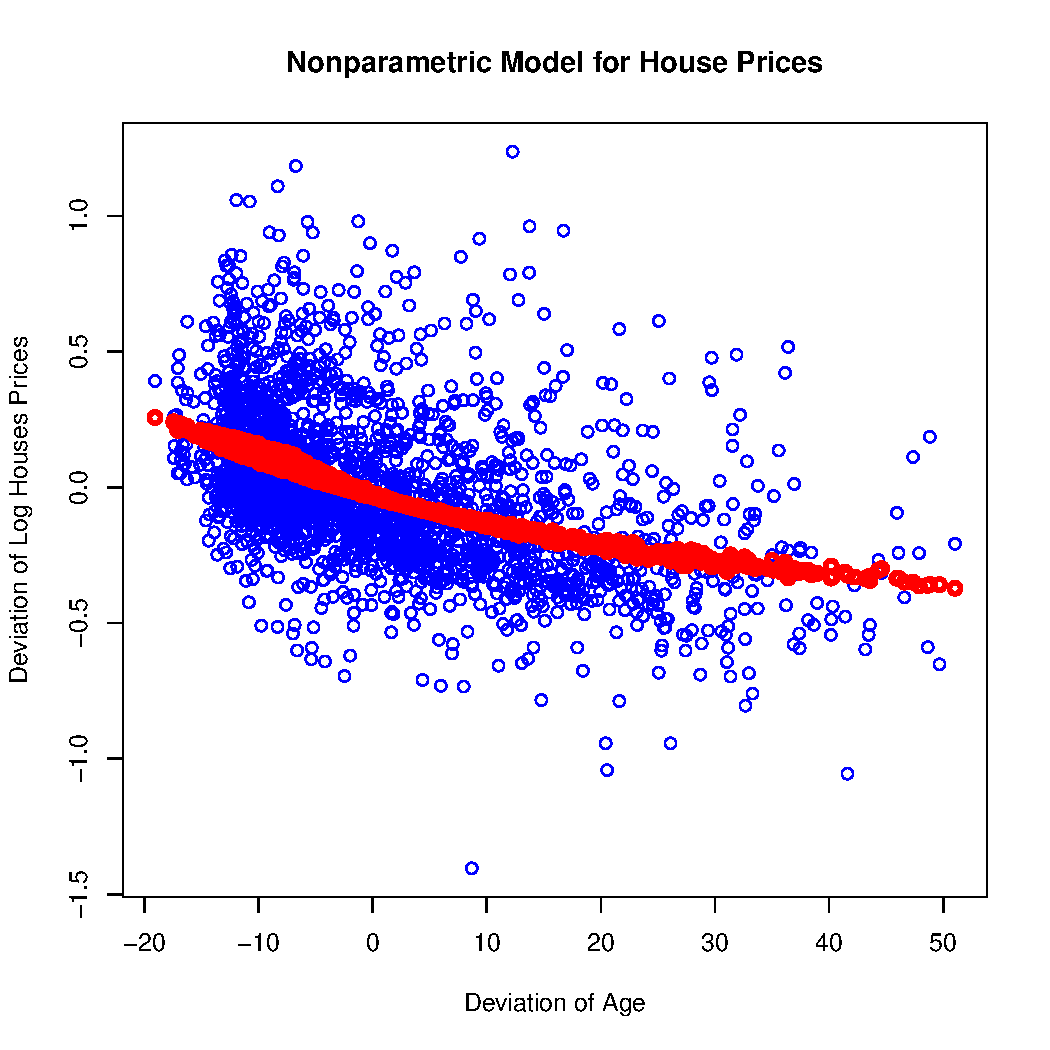
\includegraphics[scale = 0.5, keepaspectratio=true]{../Figures/dev_vs_age_dev}
  \caption{Linear-BT Model for House Prices: Excess Age} \label{fig:dev_vs_age_dev}
\end{figure}

\clearpage
Now consider a nonparametric specification for 
the relationship between prices and age.
Figure \ref{fig:dev_np_vs_age_dev} 
overlays the nonparametric estimate (shown in green) with the above in 
Figure \ref{fig:dev_vs_age_dev}.
The pattern has more variation in slope but 
closely follows the prediction from the BT model. 
So far, it appears that the BT form
is close enough.

\begin{figure}[h!]
  \centering
  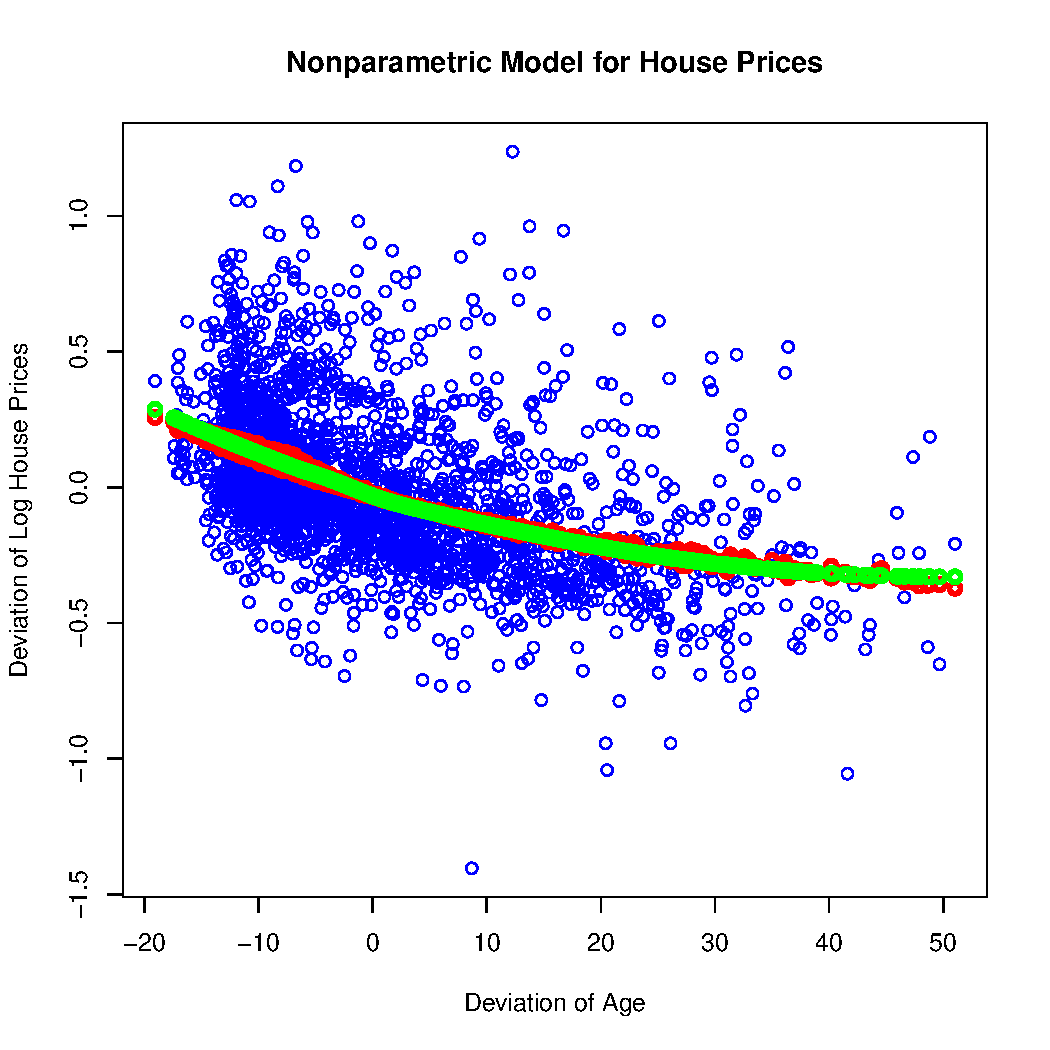
\includegraphics[scale = 0.5, keepaspectratio=true]{../Figures/dev_np_vs_age_dev}
  \caption{Nonparametric Model for House Prices: Excess Age} \label{fig:dev_np_vs_age_dev}
\end{figure}

 

\clearpage
Finally, consider a set of nonparametric specifications for 
the relationship between prices and age.
Figure \ref{fig:dev_np_vs_age_dev_bw} 
overlays other nonparametric estimates with the above in 
Figure \ref{fig:dev_np_vs_age_dev}.
The points in orange and in magenta represent
alternate models with different degrees of smoothing. 
%
When we estimated probability densities,
we adjusted the bandwidth parameter to fit
with different degrees of smoothness.
The \texttt{loess} method used for the nonparametric method has a span parameter for this function.
The default smoother \texttt{span} (bandwidth parameter) is 0.75.

In the magenta points, with \texttt{span} parameter 0.1, the pattern has more variation in slope but 
closely follows the prediction from the BT model. 
The smoother curve in orange 
even more closely represents a straight line. 
Again, it appears that the BT form
is close enough.
Perhaps the result will be different for other continuous variables in the model.

\begin{figure}[h!]
  \centering
  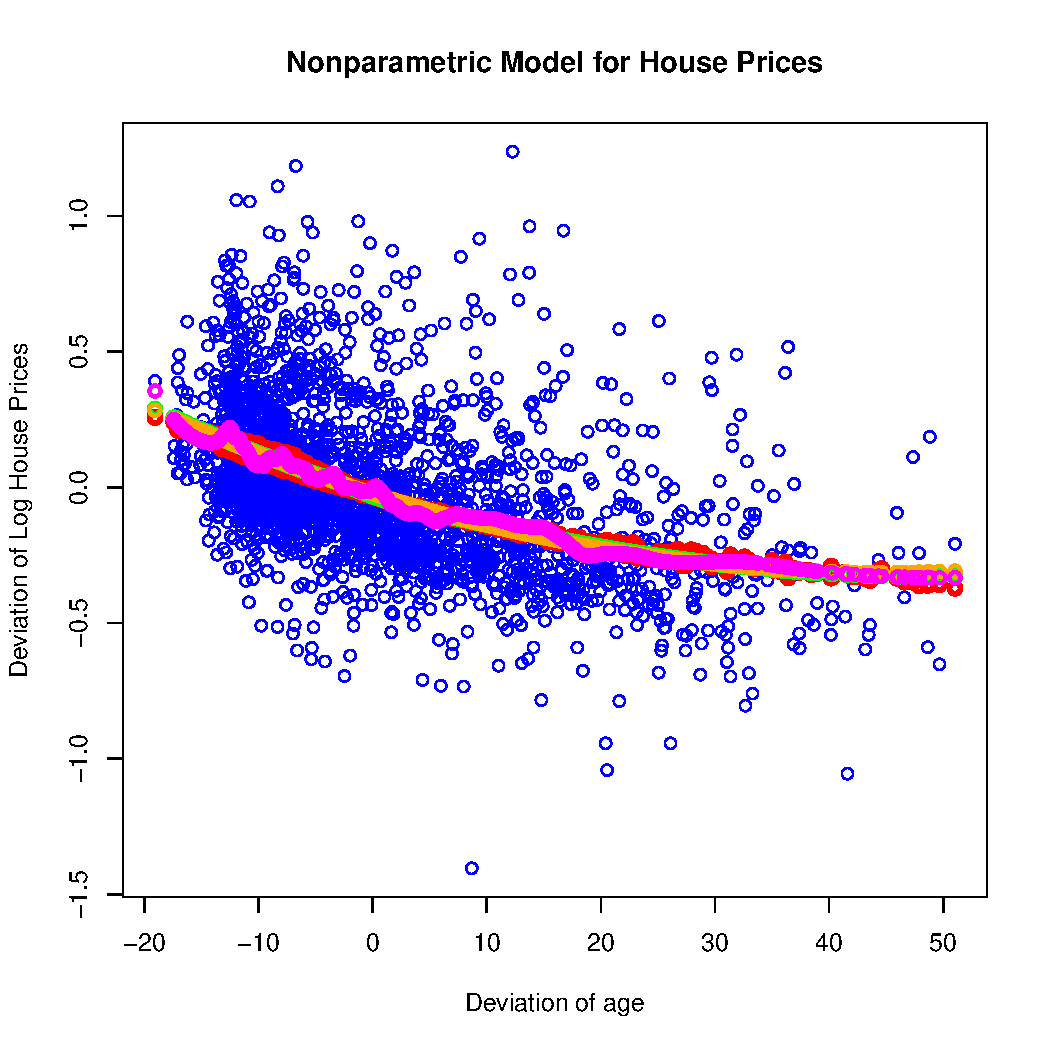
\includegraphics[scale = 0.5, keepaspectratio=true]{../Figures/dev_np_vs_age_dev_bw}
  \caption{Nonparametric Model for House Prices: Excess Age} \label{fig:dev_np_vs_age_dev_bw}
\end{figure}





\clearpage
\subsection{Nonparametric Specification for Lot Size}

As above, first conduct FWL regressions 
to reduce the problem to two dimensions. 
The models shown in
Table \ref{tab:reg_lot_fwl}
illustrate this possibility. 
Model 1 is the same original model in 
Table \ref{tab:reg_bt_age}. 
Model 2 is a regression omitting the age variable. 
Model 3 is a regression to predict age with the other explanatory variables in Model 2.
Finally, Model 4 shows the coefficient for Lot Size
from a regression of the residuals of Model 2
on the residuals from Model 3. 
Notice that these coefficients match those in Model 1. 


\begin{table}
\begin{center}
\begin{tabular}{l c c c c}
\hline
 & Original (1) & Reduced (2) & Lot Size (3) & FWL Lot Size (4) \\
\hline
(Intercept)       & $12.27956^{***}$ & $12.44426^{***}$ & $4570.55206^{***}$ &                 \\
                  & $(0.03468)$      & $(0.03096)$      & $(167.25090)$      &                 \\
TypeOfBuyerRental & $0.11437^{***}$  & $0.11974^{***}$  & $149.03169$        &                 \\
                  & $(0.01590)$      & $(0.01620)$      & $(87.51196)$       &                 \\
Age               & $-0.03428^{***}$ & $-0.03419^{***}$ & $2.63919$          &                 \\
                  & $(0.00365)$      & $(0.00372)$      & $(20.08503)$       &                 \\
NumBeds2          & $0.22090^{***}$  & $0.24652^{***}$  & $710.95724^{***}$  &                 \\
                  & $(0.02576)$      & $(0.02612)$      & $(141.13962)$      &                 \\
NumBeds3          & $0.41973^{***}$  & $0.47092^{***}$  & $1420.43656^{***}$ &                 \\
                  & $(0.03114)$      & $(0.03130)$      & $(169.09693)$      &                 \\
NumBeds4          & $0.60678^{***}$  & $0.64996^{***}$  & $1198.24876^{***}$ &                 \\
                  & $(0.03437)$      & $(0.03474)$      & $(187.71630)$      &                 \\
NumBeds6          & $0.69817^{***}$  & $0.81335^{***}$  & $3196.23145^{***}$ &                 \\
                  & $(0.05573)$      & $(0.05554)$      & $(300.08751)$      &                 \\
NumBeds8          & $1.07728^{***}$  & $1.22677^{***}$  & $4148.38835^{***}$ &                 \\
                  & $(0.06068)$      & $(0.05988)$      & $(323.52286)$      &                 \\
NumBaths2         & $0.07219^{***}$  & $0.08268^{***}$  & $290.99344^{***}$  &                 \\
                  & $(0.01376)$      & $(0.01398)$      & $(75.52624)$       &                 \\
NumBaths3         & $0.10791^{***}$  & $0.13008^{***}$  & $615.14719^{***}$  &                 \\
                  & $(0.02694)$      & $(0.02736)$      & $(147.81970)$      &                 \\
LotSize           & $0.00004^{***}$  &                  &                    &                 \\
                  & $(0.00000)$      &                  &                    &                 \\
HasGarage         & $0.26785^{***}$  & $0.34042^{***}$  & $2013.74849^{***}$ &                 \\
                  & $(0.01924)$      & $(0.01811)$      & $(97.84161)$       &                 \\
HasSecGate        & $0.22254^{***}$  & $0.22604^{***}$  & $97.24706$         &                 \\
                  & $(0.01788)$      & $(0.01822)$      & $(98.42853)$       &                 \\
TransitScore      & $0.06332^{***}$  & $0.05810^{***}$  & $-144.94653^{***}$ &                 \\
                  & $(0.00296)$      & $(0.00297)$      & $(16.03592)$       &                 \\
bt\_age\_log\_age & $0.00608^{***}$  & $0.00604^{***}$  & $-1.07046$         &                 \\
                  & $(0.00094)$      & $(0.00096)$      & $(5.17886)$        &                 \\
lot\_resid        &                  &                  &                    & $0.00004^{***}$ \\
                  &                  &                  &                    & $(0.00000)$     \\
\hline
R$^2$             & $0.67999$        & $0.66738$        & $0.56131$          & $0.03791$       \\
Adj. R$^2$        & $0.67817$        & $0.66562$        & $0.55899$          & $0.03752$       \\
Num. obs.         & $2473$           & $2473$           & $2473$             & $2473$          \\
\hline
\multicolumn{5}{l}{\scriptsize{$^{***}p<0.001$; $^{**}p<0.01$; $^{*}p<0.05$}}
\end{tabular}
\caption{Linear Model for Lot Size: FWL Regressions}
\label{tab:reg_lot_fwl}
\end{center}
\end{table}


\pagebreak 
To illustrate the fit of the model, 
Figure \ref{fig:dev_vs_lot} shows a scatter plot 
of the residual log prices on Lot Size. 
The observations are shown in blue
and the fitted values are shown in red.
The variation in the fitted values results from the 
fact that it is not plotted against the transformed excess lot size variable used in the regressions.
Still, the linear pattern is apparent
and appears to match the data. 

\begin{figure}[h!]
  \centering
  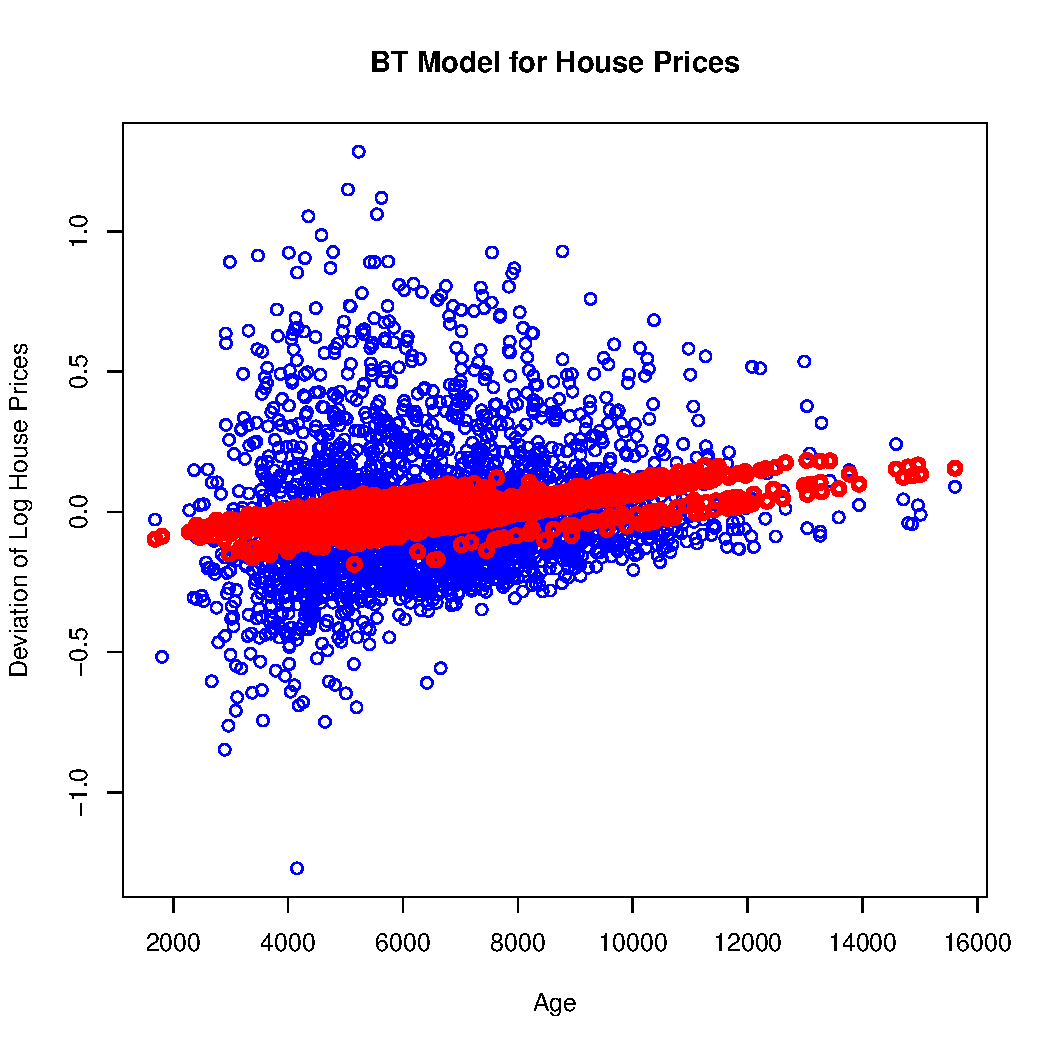
\includegraphics[scale = 0.5, keepaspectratio=true]{../Figures/dev_vs_lot}
  \caption{Linear-BT Model for House Prices} \label{fig:dev_vs_lot}
\end{figure}



\pagebreak
As a comparison, Figure \ref{fig:dev_vs_lot_dev} 
augments the above by showing the plot against the 
residuals from the regression for lot size:
the ``excess lot size'' of a house compared to what would be 
expected given the other characteristics of the hosue. 


\begin{figure}[h!]
  \centering
  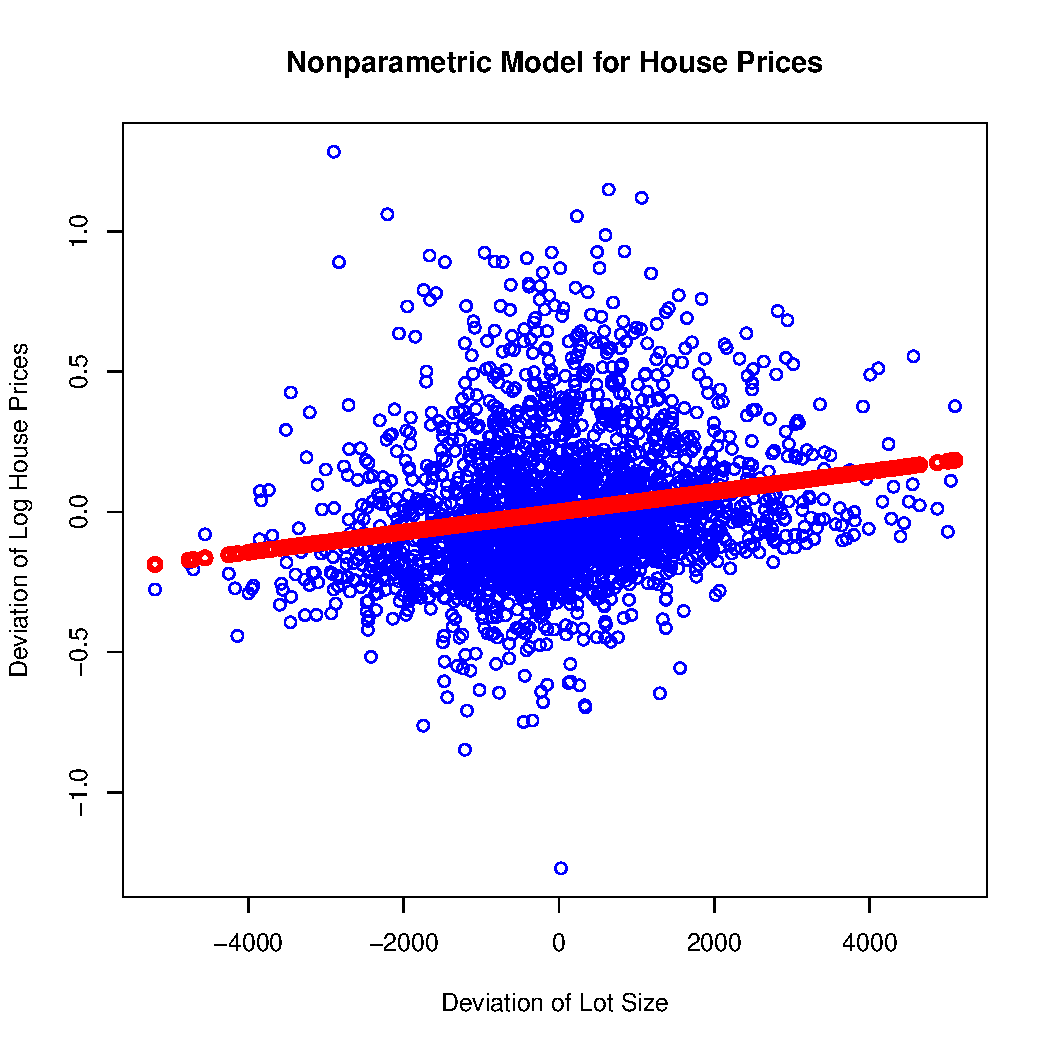
\includegraphics[scale = 0.5, keepaspectratio=true]{../Figures/dev_vs_lot_dev}
  \caption{Linear-BT Model for House Prices: Excess Lot Size} \label{fig:dev_vs_lot_dev}
\end{figure}

\clearpage
Now consider a nonparametric specification for 
the relationship between prices and Lot Size.
Figure \ref{fig:dev_np_vs_lot_dev} 
overlays the nonparametric estimate (shown in green) with the above in 
Figure \ref{fig:dev_vs_lot_dev}.
The pattern has more variation in slope but 
closely follows the prediction from the linear model. 
Although the nonparametric estimate varies around the linear estimate,
it appears that the linear form
is a close enough approximation without the added complexity.
Next, I will explore the transit score variable.


\begin{figure}[h!]
  \centering
  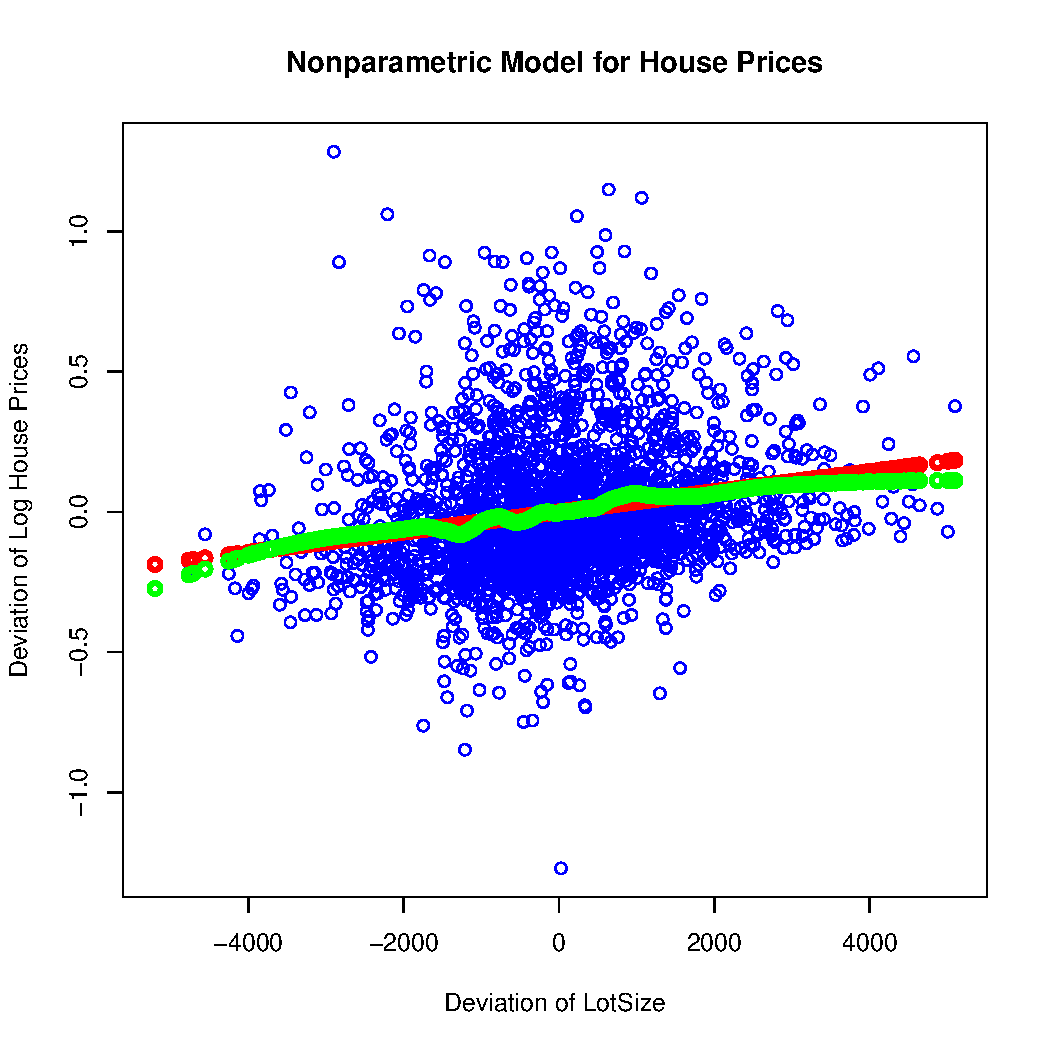
\includegraphics[scale = 0.5, keepaspectratio=true]{../Figures/dev_np_vs_lot_dev}
  \caption{Nonparametric Model for House Prices: Excess Lot Size} \label{fig:dev_np_vs_lot_dev}
\end{figure}





\clearpage
\subsection{Nonparametric Specification for Transit Score}

As above, first conduct FWL regressions 
to reduce the problem to two dimensions. 
The models shown in
Table \ref{tab:reg_trans_fwl}
illustrate this possibility. 
Model 1 is the same original model in 
Table \ref{tab:reg_bt_age}. 
Model 2 is a regression omitting the transit score variable. 
Model 3 is a regression to predict transit score with the other explanatory variables in Model 2.
Finally, Model 4 shows the coefficient for trasnit score
from a regression of the residuals of Model 2
on the residuals from Model 3. 
Notice that these coefficients match those in Model 1. 


\begin{table}
\begin{center}
\begin{tabular}{l c c c c}
\hline
 & Original (1) & Reduced (2) & Transit. (3) & FWL Transit (4) \\
\hline
(Intercept)       & $12.27956^{***}$ & $12.63639^{***}$ & $3.30691^{***}$  &                 \\
                  & $(0.03468)$      & $(0.03156)$      & $(0.19943)$      &                 \\
TypeOfBuyerRental & $0.11437^{***}$  & $0.16789^{***}$  & $0.82865^{***}$  &                 \\
                  & $(0.01590)$      & $(0.01721)$      & $(0.10875)$      &                 \\
Age               & $-0.03428^{***}$ & $-0.03571^{***}$ & $-0.02614$       &                 \\
                  & $(0.00365)$      & $(0.00399)$      & $(0.02525)$      &                 \\
NumBeds2          & $0.22090^{***}$  & $0.38493^{***}$  & $2.38241^{***}$  &                 \\
                  & $(0.02576)$      & $(0.02703)$      & $(0.17083)$      &                 \\
NumBeds3          & $0.41973^{***}$  & $0.68120^{***}$  & $3.61940^{***}$  &                 \\
                  & $(0.03114)$      & $(0.03160)$      & $(0.19969)$      &                 \\
NumBeds4          & $0.60678^{***}$  & $0.55368^{***}$  & $-1.65707^{***}$ &                 \\
                  & $(0.03437)$      & $(0.03697)$      & $(0.23364)$      &                 \\
NumBeds6          & $0.69817^{***}$  & $0.69526^{***}$  & $-2.03272^{***}$ &                 \\
                  & $(0.05573)$      & $(0.05935)$      & $(0.37507)$      &                 \\
NumBeds8          & $1.07728^{***}$  & $1.09572^{***}$  & $-2.25567^{***}$ &                 \\
                  & $(0.06068)$      & $(0.06396)$      & $(0.40421)$      &                 \\
NumBaths2         & $0.07219^{***}$  & $0.08315^{***}$  & $0.00810$        &                 \\
                  & $(0.01376)$      & $(0.01503)$      & $(0.09496)$      &                 \\
NumBaths3         & $0.10791^{***}$  & $0.12951^{***}$  & $-0.00978$       &                 \\
                  & $(0.02694)$      & $(0.02941)$      & $(0.18585)$      &                 \\
LotSize           & $0.00004^{***}$  &                  &                  &                 \\
                  & $(0.00000)$      &                  &                  &                 \\
HasGarage         & $0.26785^{***}$  & $0.34991^{***}$  & $0.16338$        &                 \\
                  & $(0.01924)$      & $(0.01946)$      & $(0.12297)$      &                 \\
HasSecGate        & $0.22254^{***}$  & $0.22158^{***}$  & $-0.07681$       &                 \\
                  & $(0.01788)$      & $(0.01958)$      & $(0.12374)$      &                 \\
TransitScore      & $0.06332^{***}$  &                  &                  &                 \\
                  & $(0.00296)$      &                  &                  &                 \\
bt\_age\_log\_age & $0.00608^{***}$  & $0.00634^{***}$  & $0.00507$        &                 \\
                  & $(0.00094)$      & $(0.00103)$      & $(0.00651)$      &                 \\
trans\_resid      &                  &                  &                  & $0.05810^{***}$ \\
                  &                  &                  &                  & $(0.00296)$     \\
\hline
R$^2$             & $0.67999$        & $0.61555$        & $0.62322$        & $0.13481$       \\
Adj. R$^2$        & $0.67817$        & $0.61368$        & $0.62138$        & $0.13446$       \\
Num. obs.         & $2473$           & $2473$           & $2473$           & $2473$          \\
\hline
\multicolumn{5}{l}{\scriptsize{$^{***}p<0.001$; $^{**}p<0.01$; $^{*}p<0.05$}}
\end{tabular}
\caption{Linear Model for Transit Score: FWL Regressions}
\label{tab:reg_trans_fwl}
\end{center}
\end{table}


\pagebreak 
To illustrate the fit of the model, 
Figure \ref{fig:dev_vs_trans} shows a scatter plot 
of the residual log prices on transit score. 
The observations are shown in blue
and the fitted values are shown in red.
The variation in the fitted values results from the 
fact that it is not plotted against the transformed excess transit score variable used in the regressions.
Still, the linear pattern is apparent
and appears to match the data. 

\begin{figure}[h!]
  \centering
  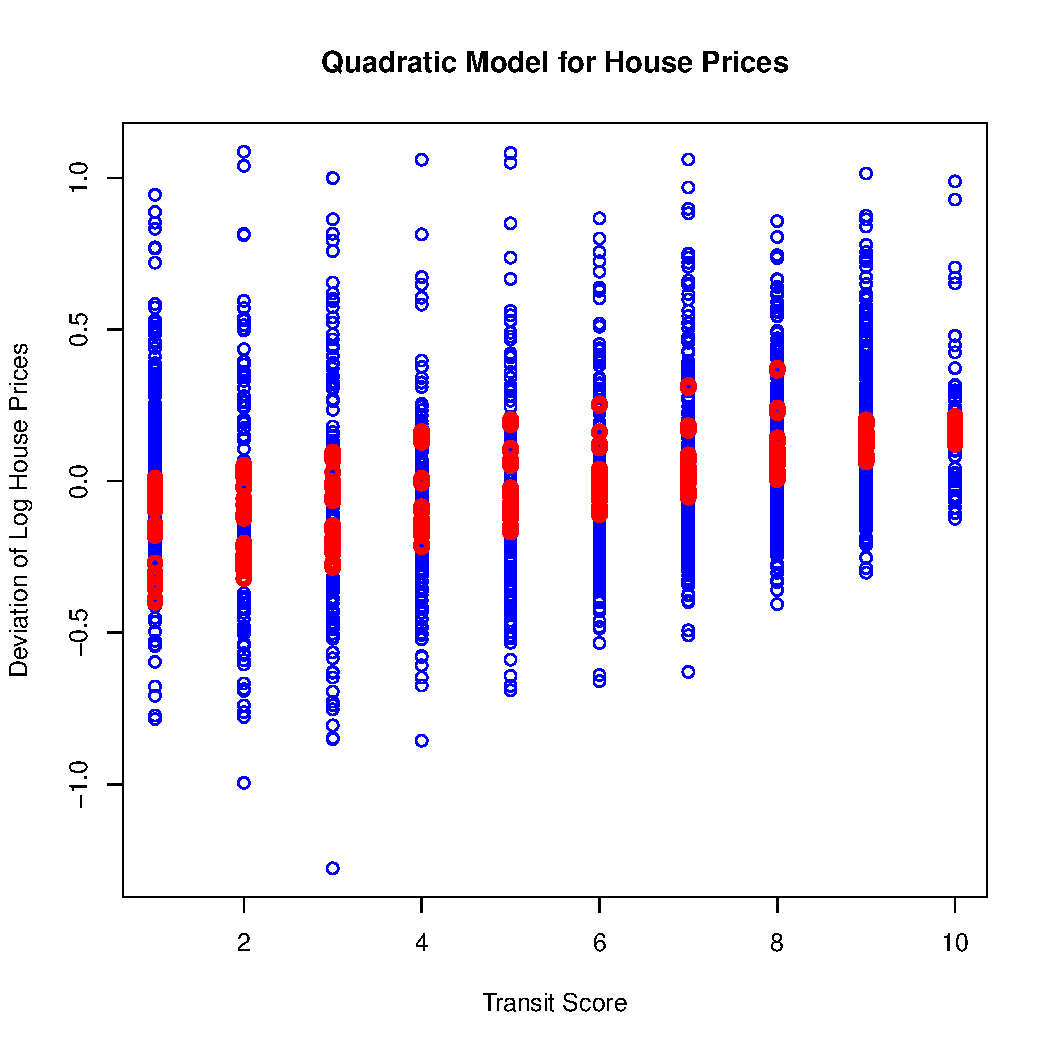
\includegraphics[scale = 0.5, keepaspectratio=true]{../Figures/dev_vs_trans}
  \caption{Linear-BT Model for House Prices} \label{fig:dev_vs_trans}
\end{figure}



\pagebreak
As a comparison, Figure \ref{fig:dev_np_vs_trans_dev} 
augments the above by showing the plot against the 
residuals from the regression for age:
the ``excess transit score'' of a house compared to what would be 
expected given the other characteristics of the house. 

% 
I move directly to the nonparametric specification for 
the relationship between prices and transit score.
Figure \ref{fig:dev_np_vs_trans_dev} 
overlays the nonparametric estimate, shown in green. 



\begin{figure}[h!]
  \centering
  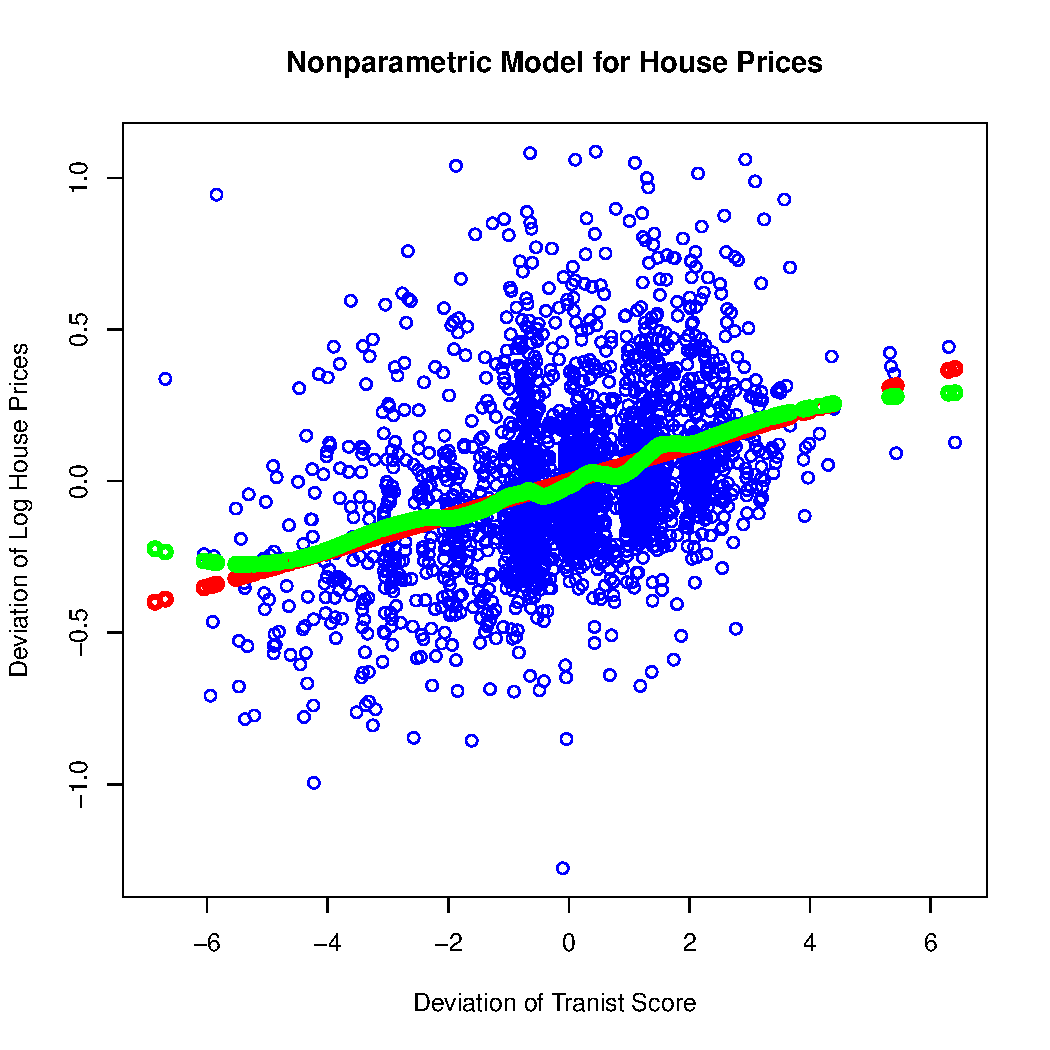
\includegraphics[scale = 0.5, keepaspectratio=true]{../Figures/dev_np_vs_trans_dev}
  \caption{Nonparametric Model for House Prices: Excess Transit Score} \label{fig:dev_np_vs_trans_dev}
\end{figure}

 

\pagebreak
\section{Semiparametric Estimates}

As I was building the above nonparametric models, 
I stored the predictions and will now use them as variables in 
linear models. 
Table \ref{tab:reg_semipar} 
shows the estimates from a set of models. 
Model 1 is the benchmark linear model in 
Table \ref{tab:reg_bt_age}. 
Model 2 is a semi-parametric model
with a nonparametric fit on age
substituted in for the age variables.
Models 3 and 4 are semi-parametric models
with nonparametric fits on lot size and transit score, respectively.
Model 5 is a maximally semiparametric model, 
with nonparametric fits for all continuous variables. 
For each of the single-variable semiparametric models, 
the coefficients are near one
and the fits are similar to the linear model. 
Even with maximal flexibility, the fit of Model 5
is not much better than the benchmark linear model. 
Across models 1, 4 and 5, the adjusted $\bar{R}^2$ values are all hovering around 0.62. 
All things considered, these are excellent models
and the linear model is sufficient.


\begin{table}
\begin{center}
\begin{tabular}{l c c c c c}
\hline
 & Model 1 & Model 2 & Model 3 & Model 4 & Model 5 \\
\hline
(Intercept)       & $12.27956^{***}$ & $12.46848^{***}$ & $12.63542^{***}$ & $12.63901^{***}$ & $12.47247^{***}$ \\
                  & $(0.03468)$      & $(0.02944)$      & $(0.03100)$      & $(0.02928)$      & $(0.02643)$      \\
TypeOfBuyerRental & $0.11437^{***}$  & $0.09463^{***}$  & $0.16816^{***}$  & $0.16510^{***}$  & $0.09156^{***}$  \\
                  & $(0.01590)$      & $(0.01725)$      & $(0.01690)$      & $(0.01597)$      & $(0.01549)$      \\
Age               & $-0.03428^{***}$ &                  & $-0.03531^{***}$ & $-0.03555^{***}$ &                  \\
                  & $(0.00365)$      &                  & $(0.00392)$      & $(0.00371)$      &                  \\
NumBeds2          & $0.22090^{***}$  & $0.39266^{***}$  & $0.38449^{***}$  & $0.37968^{***}$  & $0.38653^{***}$  \\
                  & $(0.02576)$      & $(0.02737)$      & $(0.02655)$      & $(0.02508)$      & $(0.02457)$      \\
NumBeds3          & $0.41973^{***}$  & $0.69266^{***}$  & $0.68003^{***}$  & $0.67808^{***}$  & $0.68809^{***}$  \\
                  & $(0.03114)$      & $(0.03200)$      & $(0.03104)$      & $(0.02932)$      & $(0.02872)$      \\
NumBeds4          & $0.60678^{***}$  & $0.55581^{***}$  & $0.55357^{***}$  & $0.54859^{***}$  & $0.55004^{***}$  \\
                  & $(0.03437)$      & $(0.03744)$      & $(0.03632)$      & $(0.03430)$      & $(0.03361)$      \\
NumBeds6          & $0.69817^{***}$  & $0.70465^{***}$  & $0.69855^{***}$  & $0.71472^{***}$  & $0.72890^{***}$  \\
                  & $(0.05573)$      & $(0.06010)$      & $(0.05830)$      & $(0.05507)$      & $(0.05396)$      \\
NumBeds8          & $1.07728^{***}$  & $1.15277^{***}$  & $1.10040^{***}$  & $1.10802^{***}$  & $1.17134^{***}$  \\
                  & $(0.06068)$      & $(0.06475)$      & $(0.06283)$      & $(0.05934)$      & $(0.05813)$      \\
NumBaths2         & $0.07219^{***}$  & $0.08847^{***}$  & $0.08286^{***}$  & $0.08323^{***}$  & $0.08830^{***}$  \\
                  & $(0.01376)$      & $(0.01522)$      & $(0.01476)$      & $(0.01394)$      & $(0.01366)$      \\
NumBaths3         & $0.10791^{***}$  & $0.13918^{***}$  & $0.12915^{***}$  & $0.12929^{***}$  & $0.13893^{***}$  \\
                  & $(0.02694)$      & $(0.02977)$      & $(0.02889)$      & $(0.02728)$      & $(0.02672)$      \\
LotSize           & $0.00004^{***}$  &                  &                  &                  &                  \\
                  & $(0.00000)$      &                  &                  &                  &                  \\
HasGarage         & $0.26785^{***}$  & $0.29027^{***}$  & $0.35095^{***}$  & $0.34982^{***}$  & $0.29112^{***}$  \\
                  & $(0.01924)$      & $(0.01959)$      & $(0.01912)$      & $(0.01805)$      & $(0.01759)$      \\
HasSecGate        & $0.22254^{***}$  & $0.18970^{***}$  & $0.22175^{***}$  & $0.22100^{***}$  & $0.18897^{***}$  \\
                  & $(0.01788)$      & $(0.01980)$      & $(0.01923)$      & $(0.01817)$      & $(0.01777)$      \\
TransitScore      & $0.06332^{***}$  &                  &                  &                  &                  \\
                  & $(0.00296)$      &                  &                  &                  &                  \\
bt\_age\_log\_age & $0.00608^{***}$  &                  & $0.00623^{***}$  & $0.00630^{***}$  &                  \\
                  & $(0.00094)$      &                  & $(0.00101)$      & $(0.00096)$      &                  \\
age\_np           &                  & $0.98989^{***}$  &                  &                  & $1.03645^{***}$  \\
                  &                  & $(0.04111)$      &                  &                  & $(0.03695)$      \\
lot\_np           &                  &                  & $1.00375^{***}$  &                  & $1.06134^{***}$  \\
                  &                  &                  & $(0.10570)$      &                  & $(0.09782)$      \\
trans\_np         &                  &                  &                  & $1.02370^{***}$  & $1.10299^{***}$  \\
                  &                  &                  &                  & $(0.05125)$      & $(0.05028)$      \\
\hline
R$^2$             & $0.67999$        & $0.60556$        & $0.62915$        & $0.66923$        & $0.68242$        \\
Adj. R$^2$        & $0.67817$        & $0.60380$        & $0.62719$        & $0.66748$        & $0.68074$        \\
Num. obs.         & $2473$           & $2473$           & $2473$           & $2473$           & $2473$           \\
\hline
\multicolumn{6}{l}{\scriptsize{$^{***}p<0.001$; $^{**}p<0.01$; $^{*}p<0.05$}}
\end{tabular}
\caption{Semiparametric Models for House Prices}
\label{tab:reg_semipar}
\end{center}
\end{table}






\pagebreak
\section{Generalized Additive Model}

\subsection{Linear Model}

As an example of the output from the GAM specification, 
I first estimated the model with no nonlinear terms, 
which is essentially a linear regression. 

\begin{verbatim}
Family: gaussian 
Link function: identity 

Formula:
log_Price ~ TypeOfBuyer + NumBeds + NumBaths + HasGarage + HasSecGate + 
    bt_age_log_age + Age

Parametric coefficients:
                   Estimate Std. Error t value Pr(>|t|)    
(Intercept)       12.636387   0.031557 400.428  < 2e-16 ***
TypeOfBuyerRental  0.167885   0.017208   9.756  < 2e-16 ***
NumBeds2           0.384933   0.027031  14.240  < 2e-16 ***
NumBeds3           0.681198   0.031598  21.559  < 2e-16 ***
NumBeds4           0.553684   0.036969  14.977  < 2e-16 ***
NumBeds6           0.695256   0.059348  11.715  < 2e-16 ***
NumBeds8           1.095722   0.063960  17.131  < 2e-16 ***
NumBaths2          0.083150   0.015026   5.534 3.46e-08 ***
NumBaths3          0.129513   0.029408   4.404 1.11e-05 ***
HasGarage          0.349911   0.019458  17.983  < 2e-16 ***
HasSecGate         0.221579   0.019581  11.316  < 2e-16 ***
bt_age_log_age     0.006339   0.001030   6.153 8.86e-10 ***
Age               -0.035709   0.003995  -8.938  < 2e-16 ***
---
Signif. codes:  0 �***� 0.001 �**� 0.01 �*� 0.05 �.� 0.1 � � 1


R-sq.(adj) =  0.614   Deviance explained = 61.6%
GCV = 0.077393  Scale est. = 0.076987  n = 2473
\end{verbatim}

\pagebreak
\subsection{Semiparametric Model}


Further investigating the results of the full semiparametric specification
of Model 5 of Table \ref{tab:reg_semipar},
I estimated the model with all three continuous variables specified as nonparametric functions. 
The result was that 
almost all the variables---both linear and nonlinear---were 
statistically significant. 


\begin{verbatim}
Family: gaussian 
Link function: identity 

Formula:
log_Price ~ s(Age) + s(LotSize) + s(TransitScore) + TypeOfBuyer + 
    NumBeds + NumBaths + HasGarage + HasSecGate

Parametric coefficients:
                  Estimate Std. Error t value Pr(>|t|)    
(Intercept)       12.66687    0.03019 419.567  < 2e-16 ***
TypeOfBuyerRental  0.11042    0.01605   6.880 7.59e-12 ***
NumBeds2           0.21419    0.02606   8.218 3.31e-16 ***
NumBeds3           0.40513    0.03149  12.865  < 2e-16 ***
NumBeds4           0.58441    0.03644  16.037  < 2e-16 ***
NumBeds6           0.69712    0.05784  12.053  < 2e-16 ***
NumBeds8           1.08605    0.06412  16.938  < 2e-16 ***
NumBaths2          0.07120    0.01373   5.186 2.32e-07 ***
NumBaths3          0.10819    0.02686   4.027 5.81e-05 ***
HasGarage          0.25377    0.01974  12.856  < 2e-16 ***
HasSecGate         0.22450    0.01785  12.576  < 2e-16 ***
---
Signif. codes:  0 �***� 0.001 �**� 0.01 �*� 0.05 �.� 0.1 � � 1

Approximate significance of smooth terms:
                  edf Ref.df      F p-value    
s(Age)          2.893  3.614 201.80  <2e-16 ***
s(LotSize)      3.127  4.010  27.57  <2e-16 ***
s(TransitScore) 2.989  3.756 126.22  <2e-16 ***
---
Signif. codes:  0 �***� 0.001 �**� 0.01 �*� 0.05 �.� 0.1 � � 1

R-sq.(adj) =   0.68   Deviance explained = 68.3%
GCV = 0.06425  Scale est. = 0.063731  n = 2473
\end{verbatim}

On the other hand, 
the adjusted R-squared has decreased
from 0.68 to 0.614 under this specification, 
which therefore suggests this complex model is not efficient as the more simpler one.


Perhaps as a middle ground, we can estimate a model with a 
nonparametric specification for the age variable alone, 
since it seems to have a nonlinear relationship with value in either case. 
This retains most of the predictive value of the maximally 
semiparametric model and accommodates the 
nonlinear relationship with value of age. This brought the adjusted R Squared back up to .68 but still the model is too complex to be chosen and the original model chosen in Problem Set 7 should be used.

\begin{verbatim}
Family: gaussian 
Link function: identity 

Formula:
log_Price ~ s(Age) + LotSize + TransitScore + TypeOfBuyer + NumBeds + 
    NumBaths + HasGarage + HasSecGate

Parametric coefficients:
                   Estimate Std. Error t value Pr(>|t|)    
(Intercept)       1.206e+01  3.275e-02 368.273  < 2e-16 ***
LotSize           3.606e-05  3.665e-06   9.839  < 2e-16 ***
TransitScore      6.339e-02  2.963e-03  21.397  < 2e-16 ***
TypeOfBuyerRental 1.145e-01  1.592e-02   7.195 8.24e-13 ***
NumBeds2          2.201e-01  2.578e-02   8.535  < 2e-16 ***
NumBeds3          4.191e-01  3.117e-02  13.447  < 2e-16 ***
NumBeds4          6.070e-01  3.440e-02  17.648  < 2e-16 ***
NumBeds6          6.992e-01  5.579e-02  12.532  < 2e-16 ***
NumBeds8          1.076e+00  6.073e-02  17.720  < 2e-16 ***
NumBaths2         7.248e-02  1.377e-02   5.264 1.53e-07 ***
NumBaths3         1.078e-01  2.696e-02   3.997 6.59e-05 ***
HasGarage         2.675e-01  1.925e-02  13.895  < 2e-16 ***
HasSecGate        2.226e-01  1.789e-02  12.441  < 2e-16 ***
---
Signif. codes:  0 �***� 0.001 �**� 0.01 �*� 0.05 �.� 0.1 � � 1

Approximate significance of smooth terms:
         edf Ref.df     F p-value    
s(Age) 2.908  3.632 198.3  <2e-16 ***
---
Signif. codes:  0 �***� 0.001 �**� 0.01 �*� 0.05 �.� 0.1 � � 1

R-sq.(adj) =  0.678   Deviance explained =   68%
GCV = 0.064646  Scale est. = 0.06423   n = 2473
\end{verbatim}



%%%%%%%%%%%%%%%%%%%%%%%%%%%%%%%%%%%%%%%%
%\end{document}
%%%%%%%%%%%%%%%%%%%%%%%%%%%%%%%%%%%%%%%%


\pagebreak
\chapter{Sample Selection Models}
%\documentclass[11pt]{paper}
%\usepackage{fullpage}
%\usepackage{palatino}
%\usepackage{amsfonts,amsmath,amssymb}
%% \usepackage{graphicx}
%
%\usepackage{listings}
%\usepackage{textcomp}
%\usepackage{color}
%
%\definecolor{dkgreen}{rgb}{0,0.6,0}
%\definecolor{gray}{rgb}{0.5,0.5,0.5}
%\definecolor{mauve}{rgb}{0.58,0,0.82}
%
%\lstset{frame=tb,
%  language=R,
%  aboveskip=3mm,
%  belowskip=3mm,
%  showstringspaces=false,
%  columns=flexible,
%  basicstyle={\small\ttfamily},
%  numbers=none,
%  numberstyle=\tiny\color{gray},
%  keywordstyle=\color{blue},
%  commentstyle=\color{dkgreen},
%  stringstyle=\color{mauve},
%  breaklines=true,
%  breakatwhitespace=true,
%  tabsize=3
%}
%
%
%
%\ifx\pdftexversion\undefined
%    \usepackage[dvips]{graphicx}
%\else
%    \usepackage[pdftex]{graphicx}
%    \usepackage{epstopdf}
%    \epstopdfsetup{suffix=}
%\fi
%
%\usepackage{subfig}
%
%
%% This allows pdflatex to print the curly quotes in the
%% significance codes in the output of the GAM.
%\UseRawInputEncoding
%
%\begin{document}
%
%%%%%%%%%%%%%%%%%%%%%%%%%%%%%%%%%%%%%%%%%
%% Problem Set 10
%%%%%%%%%%%%%%%%%%%%%%%%%%%%%%%%%%%%%%%%%
%
%\pagestyle{empty}
%{\noindent\bf Spring 2023 \hfill Brandon~Parmanand}
%\vskip 16pt
%\centerline{\bf University of Central Florida}
%\centerline{\bf College of Business}
%\vskip 16pt
%\centerline{\bf QMB 6911}
%\centerline{\bf Capstone Project in Business Analytics}
%\vskip 10pt
%\centerline{\bf Solutions:  Problem Set \#10}
%\vskip 32pt
%\noindent
%% 
%\section{Data Description}
%
%This analysis follows the script \texttt{PS10.R} to produce a more accurate model for used tractor prices with the data from \texttt{homesales.dat} in the \texttt{Data} folder. 
%

I will revisit the recommended linear model in which we
considered other nonlinear specifications
within a Generalized Additive Model. 

Then I will further investigate this nonlinear relationship
by considering the issue of sample selection:
whether a house will be owner occupied or a rental.


%%%%%%%%%%%%%%%%%%%%%%%%%%%%%%%%%%%%%%%%
\clearpage
\section{Linear Regression Model}
%%%%%%%%%%%%%%%%%%%%%%%%%%%%%%%%%%%%%%%%

My starting point is my recommended linear model
in which I used a box tidwell transformation for age and it is shown in Table \ref{tab:reg_bt_age}.

% 

\begin{table}
\begin{center}
\begin{tabular}{l c}
\hline
 & Model 1 \\
\hline
(Intercept)       & $12.27956^{***}$ \\
                  & $(0.03468)$      \\
TypeOfBuyerRental & $0.11437^{***}$  \\
                  & $(0.01590)$      \\
Age               & $-0.03428^{***}$ \\
                  & $(0.00365)$      \\
NumBeds2          & $0.22090^{***}$  \\
                  & $(0.02576)$      \\
NumBeds3          & $0.41973^{***}$  \\
                  & $(0.03114)$      \\
NumBeds4          & $0.60678^{***}$  \\
                  & $(0.03437)$      \\
NumBeds6          & $0.69817^{***}$  \\
                  & $(0.05573)$      \\
NumBeds8          & $1.07728^{***}$  \\
                  & $(0.06068)$      \\
NumBaths2         & $0.07219^{***}$  \\
                  & $(0.01376)$      \\
NumBaths3         & $0.10791^{***}$  \\
                  & $(0.02694)$      \\
LotSize           & $0.00004^{***}$  \\
                  & $(0.00000)$      \\
HasGarage         & $0.26785^{***}$  \\
                  & $(0.01924)$      \\
HasSecGate        & $0.22254^{***}$  \\
                  & $(0.01788)$      \\
TransitScore      & $0.06332^{***}$  \\
                  & $(0.00296)$      \\
bt\_age\_log\_age & $0.00608^{***}$  \\
                  & $(0.00094)$      \\
\hline
R$^2$             & $0.67999$        \\
Adj. R$^2$        & $0.67817$        \\
Num. obs.         & $2473$           \\
\hline
\multicolumn{2}{l}{\scriptsize{$^{***}p<0.001$; $^{**}p<0.01$; $^{*}p<0.05$}}
\end{tabular}
\caption{Age BT Model for Home Prices}
\label{tab:reg_bt_age}
\end{center}
\end{table}

% 

I will attempt to improve on this specification, 
using Tobit models for sample selection. 

\clearpage
%%%%%%%%%%%%%%%%%%%%%%%%%%%%%%%%%%%%%%%%
% \pagebreak
\subsubsection{Separate Models by Brand}
%%%%%%%%%%%%%%%%%%%%%%%%%%%%%%%%%%%%%%%%

To test for many possible differences in the 
models by types of buyers, 
Table \ref{tab:reg_TypeOfBuyer}
shows the estimates for two separate models
by type of buyer ownership.
%
Model 1 shows the estimates for 
the full sample,
Model 2 shows the estimates from the full model for 
Owner Occupied Buyers
and Model 4 and
represents rental buyers. 
% 
Models 3 and 5 show the estimates from a reduced version of each model, 
in which all coefficients are statistically significant. 
% 
The coefficients appear similar across the two subsamples.
Notable differences include the statistical significance for 
the indicators for number of beds, number of baths, a securit gate, transit score and garage.


\begin{table}
\begin{center}
\begin{tabular}{l c c c c c}
\hline
 & Model 1 & Model 2 & Model 3 & Model 4 & Model 5 \\
\hline
(Intercept)       & $12.27956^{***}$ & $12.12786^{***}$ & $12.12133^{***}$ & $12.33446^{***}$ & $12.32764^{***}$ \\
                  & $(0.03468)$      & $(0.07311)$      & $(0.07331)$      & $(0.05382)$      & $(0.05408)$      \\
TypeOfBuyerRental & $0.11437^{***}$  &                  &                  &                  &                  \\
                  & $(0.01590)$      &                  &                  &                  &                  \\
Age               & $-0.03428^{***}$ & $-0.03344^{***}$ & $-0.03304^{***}$ & $-0.03619^{***}$ & $-0.03463^{***}$ \\
                  & $(0.00365)$      & $(0.00451)$      & $(0.00452)$      & $(0.00628)$      & $(0.00630)$      \\
NumBeds2          & $0.22090^{***}$  & $0.44732^{***}$  & $0.45405^{***}$  & $0.15626^{***}$  & $0.15883^{***}$  \\
                  & $(0.02576)$      & $(0.07052)$      & $(0.07070)$      & $(0.03070)$      & $(0.03086)$      \\
NumBeds3          & $0.41973^{***}$  & $0.61206^{***}$  & $0.64255^{***}$  & $0.41339^{***}$  & $0.41363^{***}$  \\
                  & $(0.03114)$      & $(0.07056)$      & $(0.07003)$      & $(0.04631)$      & $(0.04656)$      \\
NumBeds4          & $0.60678^{***}$  & $0.77542^{***}$  & $0.83483^{***}$  & $0.58897^{***}$  & $0.58869^{***}$  \\
                  & $(0.03437)$      & $(0.07159)$      & $(0.06971)$      & $(0.10147)$      & $(0.10202)$      \\
NumBeds6          & $0.69817^{***}$  & $0.87122^{***}$  & $0.94804^{***}$  & $0.49774$        & $0.50612$        \\
                  & $(0.05573)$      & $(0.08380)$      & $(0.08034)$      & $(0.31040)$      & $(0.31209)$      \\
NumBeds8          & $1.07728^{***}$  & $1.24652^{***}$  & $1.32411^{***}$  &                  &                  \\
                  & $(0.06068)$      & $(0.08680)$      & $(0.08327)$      &                  &                  \\
NumBaths2         & $0.07219^{***}$  & $0.04871^{**}$   &                  & $0.11361^{***}$  & $0.11754^{***}$  \\
                  & $(0.01376)$      & $(0.01622)$      &                  & $(0.02498)$      & $(0.02509)$      \\
NumBaths3         & $0.10791^{***}$  & $0.08593^{**}$   &                  & $0.17043$        & $0.17518$        \\
                  & $(0.02694)$      & $(0.02763)$      &                  & $(0.14374)$      & $(0.14452)$      \\
LotSize           & $0.00004^{***}$  & $0.00003^{***}$  & $0.00003^{***}$  & $0.00005^{***}$  & $0.00005^{***}$  \\
                  & $(0.00000)$      & $(0.00000)$      & $(0.00000)$      & $(0.00001)$      & $(0.00001)$      \\
HasGarage         & $0.26785^{***}$  & $0.31201^{***}$  & $0.31035^{***}$  & $0.14466^{***}$  & $0.14152^{***}$  \\
                  & $(0.01924)$      & $(0.02419)$      & $(0.02425)$      & $(0.03542)$      & $(0.03560)$      \\
HasSecGate        & $0.22254^{***}$  & $0.22191^{***}$  & $0.22300^{***}$  & $0.31187^{**}$   &                  \\
                  & $(0.01788)$      & $(0.01753)$      & $(0.01758)$      & $(0.09611)$      &                  \\
TransitScore      & $0.06332^{***}$  & $0.05572^{***}$  & $0.05561^{***}$  & $0.07211^{***}$  & $0.07254^{***}$  \\
                  & $(0.00296)$      & $(0.00374)$      & $(0.00375)$      & $(0.00486)$      & $(0.00488)$      \\
bt\_age\_log\_age & $0.00608^{***}$  & $0.00579^{***}$  & $0.00568^{***}$  & $0.00667^{***}$  & $0.00632^{***}$  \\
                  & $(0.00094)$      & $(0.00118)$      & $(0.00118)$      & $(0.00159)$      & $(0.00159)$      \\
\hline
R$^2$             & $0.67999$        & $0.57350$        & $0.57029$        & $0.68975$        & $0.68598$        \\
Adj. R$^2$        & $0.67817$        & $0.56999$        & $0.56730$        & $0.68546$        & $0.68200$        \\
Num. obs.         & $2473$           & $1594$           & $1594$           & $879$            & $879$            \\
\hline
\multicolumn{6}{l}{\scriptsize{$^{***}p<0.001$; $^{**}p<0.01$; $^{*}p<0.05$}}
\end{tabular}
\caption{Separate Models by Buyer Type}
\label{tab:reg_TypeOfBuyer}
\end{center}
\end{table}



%%%%%%%%%%%%%%%%%%%%%%%%%%%%%%%%%%%%%%%%
\clearpage
\section{Sample Selection}
%%%%%%%%%%%%%%%%%%%%%%%%%%%%%%%%%%%%%%%%


% \clearpage
\subsection{Predicting the Selection into Samples}


The specification in 
Table \ref{tab:reg_bt_age}
assumes a box tidwell functional form for
the relationship between price and age, 
without selecting into samples by type of buyer.
% 
To investigate this relationship further, 
consider the set of variables that are related to
whether or not the type of buyer is owner occupied or rental
with the characteristics observed in the dataset. 


\begin{table}
\begin{center}
\begin{tabular}{l c c}
\hline
 & Model 1 & Model 2 \\
\hline
(Intercept)                    & $-0.35769$       & $-0.93939^{***}$ \\
                               & $(0.23569)$      & $(0.16551)$      \\
Age                            & $-0.05493^{*}$   &                  \\
                               & $(0.02576)$      &                  \\
NumBeds2                       & $0.58191^{**}$   &                  \\
                               & $(0.18811)$      &                  \\
NumBeds3                       & $1.38434^{***}$  &                  \\
                               & $(0.21549)$      &                  \\
NumBeds4                       & $1.87974^{***}$  &                  \\
                               & $(0.26399)$      &                  \\
NumBeds6                       & $0.09919$        &                  \\
                               & $(0.66151)$      &                  \\
NumBeds8                       & $4.54081$        &                  \\
                               & $(74.92556)$     &                  \\
NumBaths2                      & $-0.40062^{***}$ &                  \\
                               & $(0.09378)$      &                  \\
NumBaths3                      & $-0.28703$       &                  \\
                               & $(0.28759)$      &                  \\
LotSize                        & $-0.00004$       &                  \\
                               & $(0.00003)$      &                  \\
HasGarage                      & $1.98835^{***}$  & $1.81398^{***}$  \\
                               & $(0.11192)$      & $(0.09177)$      \\
HasSecGate                     & $2.17518^{***}$  & $2.08251^{***}$  \\
                               & $(0.22948)$      & $(0.21320)$      \\
TransitScore                   & $-0.14986^{***}$ & $-0.13604^{***}$ \\
                               & $(0.02021)$      & $(0.01932)$      \\
bt\_age\_log\_age              & $0.00875$        &                  \\
                               & $(0.00661)$      &                  \\
as.factor(NumBeds == "2")TRUE  &                  & $0.52959^{**}$   \\
                               &                  & $(0.17431)$      \\
as.factor(NumBeds == "3")TRUE  &                  & $1.27798^{***}$  \\
                               &                  & $(0.19691)$      \\
as.factor(NumBeds == "4")TRUE  &                  & $1.67243^{***}$  \\
                               &                  & $(0.21402)$      \\
as.factor(NumBaths == "2")TRUE &                  & $-0.37191^{***}$ \\
                               &                  & $(0.08694)$      \\
\hline
AIC                            & $1575.28540$     & $1625.62192$     \\
BIC                            & $1656.67002$     & $1672.12742$     \\
Log Likelihood                 & $-773.64270$     & $-804.81096$     \\
Deviance                       & $1547.28540$     & $1609.62192$     \\
Num. obs.                      & $2473$           & $2473$           \\
\hline
\multicolumn{3}{l}{\scriptsize{$^{***}p<0.001$; $^{**}p<0.01$; $^{*}p<0.05$}}
\end{tabular}
\caption{Probit Models for Type of Buyer of Houses}
\label{tab:reg_probit}
\end{center}
\end{table}


Table \ref{tab:reg_probit} 
shows the estimates for a probit model to predict the selection
into samples by brand name.
% 
Model 1 in Table \ref{tab:reg_probit} 
shows a preliminary probit model to predict the selection indicator,
with all the other explanatory variables in the model.
Owner Houses are more likely to have 2-4 bedrooms, 
a garage, security gate, but less likely to have 2 bathrooms or a higher 
transit score.

% 
Model 2 shows the result of a variable-reduction exercise
to eliminate variables that are not statistically significant.
These estimates provide a concise but useful model to
indicate the houses that would be favored by owner occupied buyers.
This model is used to specify the selection equation
of the sample selection estimates investigated next. 
 
% \clearpage
\subsection{Estimating a Sample Selection Model}

In this section, I will make a valiant attempt to fit 
a sample selection model to the home sales data. 
This exercise is useful because it illustrates a level of difficulty
that is often encountered when conducting maximum likelihood estimation, 
or any for of estimation that involves numeric optimization
with a complex objective function. 

% \clearpage
\subsubsection{Sample Selection Model 1: Full Model}

For a first model, I use the entire set of variables
for both observation equations, for owner occupied and rentals.
I specify the selection equation with the variables above
from the probit model.


\begin{lstlisting}[language=R]
tobit_5_sel_1 <-
   selection(selection = Owner ~
               as.factor(NumBeds=='2') + 
               as.factor(NumBeds=='3') + as.factor(NumBeds=='4') +
               as.factor(NumBaths=='2') +
               HasGarage + HasSecGate
             + TransitScore,
             outcome = list(log_Price_rental ~
                              Age + NumBeds + NumBaths
                            + LotSize + HasGarage + HasSecGate
                            + TransitScore + bt_age_log_age,
                            log_Price_owner ~
                              Age + NumBeds + NumBaths
                            + LotSize + HasGarage + HasSecGate
                            + TransitScore + bt_age_log_age),
             iterlim = 20,
             method = '2step',
             data = homeprices)
\end{lstlisting}


\begin{lstlisting}[language=R]
R> summary(tobit_5_sel_1)
--------------------------------------------
Tobit 5 model (switching regression model)
2-step Heckman / heckit estimation
1862 observations: 621 selection 1 (0) and 1241 selection 2 (1)
42 free parameters (df = 1822)
Probit selection equation:
                               Estimate Std. Error t value Pr(>|t|)    
(Intercept)                    -0.80220    0.17676  -4.538 6.04e-06 ***
as.factor(NumBeds == "2")TRUE   0.42161    0.18592   2.268   0.0235 *  
as.factor(NumBeds == "3")TRUE   1.06384    0.20964   5.075 4.28e-07 ***
as.factor(NumBeds == "4")TRUE   1.68911    0.24903   6.783 1.59e-11 ***
as.factor(NumBaths == "2")TRUE -0.24855    0.09739  -2.552   0.0108 *  
HasGarage                       1.80620    0.09809  18.414  < 2e-16 ***
HasSecGate                      1.46611    0.18593   7.885 5.37e-15 ***
TransitScore                   -0.12937    0.02149  -6.021 2.09e-09 ***
Outcome equation 1:
                 Estimate Std. Error t value Pr(>|t|)
(Intercept)     1.230e+01         NA      NA       NA
Age            -2.467e-02         NA      NA       NA
NumBeds2        2.783e-02         NA      NA       NA
NumBeds3        1.664e-01         NA      NA       NA
NumBeds4        3.534e-01         NA      NA       NA
NumBeds6        6.822e-01         NA      NA       NA
NumBeds8               NA         NA      NA       NA
NumBaths2       1.476e-01         NA      NA       NA
NumBaths3       5.885e-02         NA      NA       NA
LotSize         4.821e-05         NA      NA       NA
HasGarage       9.135e-02         NA      NA       NA
HasSecGate      1.261e-04         NA      NA       NA
TransitScore    8.280e-02         NA      NA       NA
bt_age_log_age  4.407e-03         NA      NA       NA
Multiple R-Squared:0.6144,	Adjusted R-Squared:0.6055
Outcome equation 2:
                 Estimate Std. Error t value Pr(>|t|)
(Intercept)    12.4656275         NA      NA       NA
Age            -0.0360026         NA      NA       NA
NumBeds2        0.2056778         NA      NA       NA
NumBeds3        0.3379221         NA      NA       NA
NumBeds4        0.5375074         NA      NA       NA
NumBeds6        0.6692655         NA      NA       NA
NumBeds8        1.0587016         NA      NA       NA
NumBaths2       0.0574586         NA      NA       NA
NumBaths3       0.0679249         NA      NA       NA
LotSize         0.0000291         NA      NA       NA
HasGarage       0.2604763         NA      NA       NA
HasSecGate      0.2136549         NA      NA       NA
TransitScore    0.0612350         NA      NA       NA
bt_age_log_age  0.0065359         NA      NA       NA
Multiple R-Squared:0.5947,	Adjusted R-Squared:0.5901
   Error terms:
               Estimate Std. Error t value Pr(>|t|)
invMillsRatio1  0.10207         NA      NA       NA
invMillsRatio2 -0.09401         NA      NA       NA
sigma1          0.30703         NA      NA       NA
sigma2          0.23509         NA      NA       NA
rho1           -0.33245         NA      NA       NA
rho2           -0.39988         NA      NA       NA
--------------------------------------------
\end{lstlisting}

It returned NAs and the standard errors could not be calculated.
Furthermore, when I toggled the \texttt{method = '2step'} commented line, 
the situation did not improve, aside from returning the results from separate models as shown below. 
\begin{verbatim}
Call:
lm(formula = YO1 ~ -1 + XO1)

Residuals:
     Min       1Q   Median       3Q      Max 
-0.78380 -0.17614 -0.03691  0.14859  1.11278 

Coefficients: (1 not defined because of singularities)
                    Estimate Std. Error t value Pr(>|t|)    
XO1(Intercept)     1.231e+01  6.916e-02 177.950  < 2e-16 ***
XO1Age            -3.606e-02  6.285e-03  -5.737 1.33e-08 ***
XO1NumBeds2        1.417e-01  3.851e-02   3.680 0.000248 ***
XO1NumBeds3        3.763e-01  7.510e-02   5.012 6.55e-07 ***
XO1NumBeds4        5.031e-01  1.705e-01   2.952 0.003246 ** 
XO1NumBeds6        5.164e-01  3.119e-01   1.656 0.098170 .  
XO1NumBeds8               NA         NA      NA       NA    
XO1NumBaths2       1.264e-01  3.229e-02   3.915 9.75e-05 ***
XO1NumBaths3       1.574e-01  1.453e-01   1.083 0.278971    
XO1LotSize         4.677e-05  8.239e-06   5.677 1.87e-08 ***
XO1HasGarage       6.232e-02  1.361e-01   0.458 0.647073    
XO1HasSecGate      2.161e-01  1.805e-01   1.197 0.231539    
XO1TransitScore    7.619e-02  8.127e-03   9.374  < 2e-16 ***
XO1bt_age_log_age  6.643e-03  1.591e-03   4.176 3.27e-05 ***
XO1invMillsRatio   7.862e-02  1.255e-01   0.627 0.531024    
---
Signif. codes:  0 �***� 0.001 �**� 0.01 �*� 0.05 �.� 0.1 � � 1

Residual standard error: 0.2685 on 865 degrees of freedom
Multiple R-squared:  0.9996,	Adjusted R-squared:  0.9996 
F-statistic: 1.496e+05 on 14 and 865 DF,  p-value: < 2.2e-16


Call:
lm(formula = YO2 ~ -1 + XO2)

Residuals:
     Min       1Q   Median       3Q      Max 
-1.06431 -0.15117 -0.05538  0.09628  1.35261 

Coefficients:
                    Estimate Std. Error t value Pr(>|t|)    
XO2(Intercept)     1.229e+01  9.636e-02 127.542  < 2e-16 ***
XO2Age            -3.347e-02  4.500e-03  -7.438 1.67e-13 ***
XO2NumBeds2        3.976e-01  7.298e-02   5.448 5.91e-08 ***
XO2NumBeds3        5.265e-01  7.784e-02   6.764 1.88e-11 ***
XO2NumBeds4        6.846e-01  7.965e-02   8.596  < 2e-16 ***
XO2NumBeds6        8.120e-01  8.674e-02   9.362  < 2e-16 ***
XO2NumBeds8        1.189e+00  8.951e-02  13.279  < 2e-16 ***
XO2NumBaths2       6.192e-02  1.698e-02   3.646 0.000275 ***
XO2NumBaths3       9.613e-02  2.786e-02   3.451 0.000574 ***
XO2LotSize         3.318e-05  3.978e-06   8.341  < 2e-16 ***
XO2HasGarage       2.306e-01  3.970e-02   5.809 7.57e-09 ***
XO2HasSecGate      1.859e-01  2.239e-02   8.301  < 2e-16 ***
XO2TransitScore    6.015e-02  4.108e-03  14.640  < 2e-16 ***
XO2bt_age_log_age  5.792e-03  1.175e-03   4.930 9.11e-07 ***
XO2invMillsRatio  -1.087e-01  4.212e-02  -2.582 0.009918 ** 
---
Signif. codes:  0 �***� 0.001 �**� 0.01 �*� 0.05 �.� 0.1 � � 1

Residual standard error: 0.2413 on 1579 degrees of freedom
Multiple R-squared:  0.9997,	Adjusted R-squared:  0.9997 
F-statistic: 3.31e+05 on 15 and 1579 DF,  p-value: < 2.2e-16

\end{verbatim}
% 


\subsubsection{Sample Selection Model 2: Reduced Model from Separate Estimation}

Instead of starting with a ``big-to-small'' approach,
I reconsider the best models for each tractor brand group 
that were recommended previously .
I specify the selection equation with the variables above
from the probit model.


\begin{lstlisting}[language=R]
tobit_5_sel_2 <-
  selection(selection = Owner ~
              as.factor(NumBeds=='2') + 
              as.factor(NumBeds=='3') + as.factor(NumBeds=='4') +
              as.factor(NumBaths=='2') +
              HasGarage + HasSecGate
            + TransitScore,
            outcome = list(log_Price_rental ~
                             Age #+ NumBeds 
                           + as.factor(NumBaths=='2')
                           + LotSize #+ HasGarage + HasSecGate
                           + TransitScore + bt_age_log_age,
                           log_Price_owner ~
                             Age + NumBeds + NumBaths
                           + LotSize + HasGarage + HasSecGate
                           + TransitScore + bt_age_log_age),
            iterlim = 20,
            #method = '2step',
            data = homeprices)

\end{lstlisting}

This time there were no error messages , 
and the results were populated. 
I obtained the data from Table \ref{tab:tobit_5_sel}. 
All of the standard errors are there and all of the variables are significant.

\begin{table}
\begin{center}
\begin{tiny}
\begin{tabular}{l c}
\hline
 & Model 1 \\
\hline
S: (Intercept)                    & $-1.29026^{***}$ \\
                                  & $(0.13062)$      \\
S: as.factor(NumBeds == "2")TRUE  & $0.85339^{***}$  \\
                                  & $(0.11436)$      \\
S: as.factor(NumBeds == "3")TRUE  & $1.55339^{***}$  \\
                                  & $(0.14742)$      \\
S: as.factor(NumBeds == "4")TRUE  & $2.26678^{***}$  \\
                                  & $(0.16726)$      \\
S: as.factor(NumBaths == "2")TRUE & $-0.37745^{***}$ \\
                                  & $(0.07701)$      \\
S: HasGarage                      & $1.61799^{***}$  \\
                                  & $(0.08776)$      \\
S: HasSecGate                     & $1.74228^{***}$  \\
                                  & $(0.14921)$      \\
S: TransitScore                   & $-0.10534^{***}$ \\
                                  & $(0.01657)$      \\
O: (Intercept) (1)                & $12.29583^{***}$ \\
                                  & $(0.04348)$      \\
O: Age (1)                        & $-0.03769^{***}$ \\
                                  & $(0.00528)$      \\
O: as.factor(NumBaths == "2")TRUE & $0.18880^{***}$  \\
                                  & $(0.02260)$      \\
O: LotSize (1)                    & $0.00004^{***}$  \\
                                  & $(0.00001)$      \\
O: TransitScore (1)               & $0.09650^{***}$  \\
                                  & $(0.00430)$      \\
O: bt\_age\_log\_age (1)          & $0.00687^{***}$  \\
                                  & $(0.00133)$      \\
O: (Intercept) (2)                & $12.16596^{***}$ \\
                                  & $(0.07900)$      \\
O: Age (2)                        & $-0.03345^{***}$ \\
                                  & $(0.00449)$      \\
O: NumBeds2                       & $0.43195^{***}$  \\
                                  & $(0.07119)$      \\
O: NumBeds3                       & $0.58941^{***}$  \\
                                  & $(0.07253)$      \\
O: NumBeds4                       & $0.74995^{***}$  \\
                                  & $(0.07415)$      \\
O: NumBeds6                       & $0.85339^{***}$  \\
                                  & $(0.08462)$      \\
O: NumBeds8                       & $1.22905^{***}$  \\
                                  & $(0.08753)$      \\
O: NumBaths2                      & $0.05168^{**}$   \\
                                  & $(0.01634)$      \\
O: NumBaths3                      & $0.08828^{**}$   \\
                                  & $(0.02759)$      \\
O: LotSize (2)                    & $0.00003^{***}$  \\
                                  & $(0.00000)$      \\
O: HasGarage                      & $0.29699^{***}$  \\
                                  & $(0.02702)$      \\
O: HasSecGate                     & $0.21490^{***}$  \\
                                  & $(0.01838)$      \\
O: TransitScore (2)               & $0.05646^{***}$  \\
                                  & $(0.00377)$      \\
O: bt\_age\_log\_age (2)          & $0.00579^{***}$  \\
                                  & $(0.00117)$      \\
sigma1                            & $0.33589^{***}$  \\
                                  & $(0.00869)$      \\
sigma2                            & $0.24100^{***}$  \\
                                  & $(0.00431)$      \\
rho1                              & $-0.94812^{***}$ \\
                                  & $(0.01254)$      \\
rho2                              & $-0.09319$       \\
                                  & $(0.07580)$      \\
\hline
AIC                               & $1769.94506$     \\
BIC                               & $1955.96705$     \\
Log Likelihood                    & $-852.97253$     \\
Num. obs.                         & $2473$           \\
Censored                          & $879$            \\
Observed                          & $1594$           \\
\hline
\multicolumn{2}{l}{\tiny{$^{***}p<0.001$; $^{**}p<0.01$; $^{*}p<0.05$}}
\end{tabular}
\end{tiny}
\caption{Selection Models for House Prices}
\label{tab:tobit_5_sel}
\end{center}
\end{table}


I concede that the sample selection model has limited potential
with this dataset. 

\subsection{Discussion}

Although this outcome works with no errors and all variables are significant, the model proves to be difficult and may prove some complexities.
% 
In the end, I did succeed in finding an optimum in which the estimates were somewhat defined. We concluded that two models may not be best in the past and I stand by that decision. Owner occupied houses call for more bedrooms and bathrooms, they also prefer security and pools but the variables can be similar with higher prices for owner occupied.
The variables such as number of bedrooms may impact price but how much an investor is willing to spend on a house may be a factor as well.





%%%%%%%%%%%%%%%%%%%%%%%%%%%%%%%%%%%%%%%%
%\end{document}
%%%%%%%%%%%%%%%%%%%%%%%%%%%%%%%%%%%%%%%%


\pagebreak
\chapter{Conclusion}

In this paper I conducted a thorough analysis of the prices from sales of houses in order to investigate what characteristics of the different houses affect the pricing and dive into the rental properties versus the owner-occupied properties to develop a model best suited to estimate price.

In this paper I used various economic theories such as the market of lemons, characteristic theory, and hedonic pricing models. 
Additionally, I utilized various framework including the Tobit models for sample selection. At the end of the analysis, I suggested using the linear model
in which I used a box tidwell transformation for age and it is shown in Table \ref{tab:reg_bt_age}.
Along with the box tidwell transformation for age, we kept significant variables type of buyer, number of bedrooms, number of bathrooms, age, lot size, whether it has a garage, whether it has a security gate, and the transit score. 
These variables definitely make sense especially when determining for whether it's for a owner occupant or rental owner and correlate to pricing. With an R squared of 0.68 and adjusted R squared of 0.679, I conclude that it's a good model to estimate house prices.


\begin{table}
\begin{center}
\begin{tabular}{l c}
\hline
 & Model 1 \\
\hline
(Intercept)       & $12.27956^{***}$ \\
                  & $(0.03468)$      \\
TypeOfBuyerRental & $0.11437^{***}$  \\
                  & $(0.01590)$      \\
Age               & $-0.03428^{***}$ \\
                  & $(0.00365)$      \\
NumBeds2          & $0.22090^{***}$  \\
                  & $(0.02576)$      \\
NumBeds3          & $0.41973^{***}$  \\
                  & $(0.03114)$      \\
NumBeds4          & $0.60678^{***}$  \\
                  & $(0.03437)$      \\
NumBeds6          & $0.69817^{***}$  \\
                  & $(0.05573)$      \\
NumBeds8          & $1.07728^{***}$  \\
                  & $(0.06068)$      \\
NumBaths2         & $0.07219^{***}$  \\
                  & $(0.01376)$      \\
NumBaths3         & $0.10791^{***}$  \\
                  & $(0.02694)$      \\
LotSize           & $0.00004^{***}$  \\
                  & $(0.00000)$      \\
HasGarage         & $0.26785^{***}$  \\
                  & $(0.01924)$      \\
HasSecGate        & $0.22254^{***}$  \\
                  & $(0.01788)$      \\
TransitScore      & $0.06332^{***}$  \\
                  & $(0.00296)$      \\
bt\_age\_log\_age & $0.00608^{***}$  \\
                  & $(0.00094)$      \\
\hline
R$^2$             & $0.67999$        \\
Adj. R$^2$        & $0.67817$        \\
Num. obs.         & $2473$           \\
\hline
\multicolumn{2}{l}{\scriptsize{$^{***}p<0.001$; $^{**}p<0.01$; $^{*}p<0.05$}}
\end{tabular}
\caption{Age BT Model for Home Prices}
\label{tab:reg_bt_age}
\end{center}
\end{table}




% \end{document}

% \pagebreak
% \chapter{References}
% \input{References}


%%%%%%%%%%%%%%%%%%%%%%%%%%%%%%%%%%%%%%%%
\end{document}
%%%%%%%%%%%%%%%%%%%%%%%%%%%%%%%%%%%%%%%%
